% !TEX TS-Program = pdflatex
% arara: clean: { extensions: [ log, aux, toc, synctex.gz ] }

\documentclass[12pt,article]{memoir}

\newcommand{\course}{MA440 Precalculus}


% \usepackage{libertine}  %%%%%The Linux Libertine font family
% \usepackage[libertine]{newtxmath}

\usepackage{comicneue}
\usepackage{noto-serif}
% \usepackage{noto-mono}
\usepackage[default]{lato}
\usepackage{libertinust1math}

% \usepackage[expert,altbullet,vargreek,noamssymbols]{lucidabr}
% % \usepackage[expert,vargreek,noamssymbols]{lucbmath}
% \usepackage[amsbb,uprightoperators,subscriptcorrection,noamssymbols,mtpluscal,lucidascr]{mtpro2}

\usepackage{pifont,manfnt,bbding}

\usepackage[T1]{fontenc}
\usepackage[protrusion=true,expansion=true]{microtype}

\usepackage{amsmath}
% \usepackage{amsthm}

\usepackage[
  breaklinks = true,
  colorlinks = true,
  pdftitle = "MA440 Worksheets",
  pdfauthor = "Dr. Ye"
  ]{hyperref}

\usepackage{graphicx}
\usepackage{bookmark}
\usepackage{longtable}
\usepackage{calc}
\usepackage{booktabs}
\usepackage{array}
\usepackage{multirow}
\usepackage{multicol}
\usepackage{float}
\usepackage{colortbl}
\usepackage{pdflscape}
\usepackage{tabu}
\usepackage{tabularx}
\usepackage{threeparttable}
\usepackage{threeparttablex}
\usepackage[normalem]{ulem}
\usepackage{makecell}
\usepackage[svgnames]{xcolor}
\usepackage{import}
\usepackage{wrapfig}
\usepackage{siunitx}

% \usepackage{datetime}

\usepackage[calc,en-US]{datetime2}

\DTMnewdatestyle{lastupdated}{%
    \renewcommand{\DTMdisplaydate}[4]{%
        \number##1.\number##2.\number##3 }%
    \renewcommand{\DTMDisplaydate}{\DTMdisplaydate}%
}

\DTMnewdatestyle{moyr}{%
    \renewcommand{\DTMdisplaydate}[4]{%
    \DTMMonthname{##2}, \number##1 }%
    \renewcommand{\DTMDisplaydate}{\DTMdisplaydate}%
}

\DTMnewdatestyle{semester}% label
{
    \renewcommand{\DTMdisplaydate}[4]{%
        \ifnum##2=1
            Winter \number##1 
        \else
            \ifnum##2<6  
                Spring \number##1
            \else
                \ifnum##2<8
                    Summer \number##1
                \else
                    Fall \number##1
                \fi
            \fi
        \fi
    }%
    \renewcommand{\DTMDisplaydate}{\DTMdisplaydate}
}

\usepackage{geometry}
\geometry{
    letterpaper,
    margin=0.8in,
    % left=0.8in,
    % top=0.8in,
    % headsep=\baselineskip,
    % textwidth=26pc,
    % marginparsep=2pc,
    % marginparwidth=12pc,
    % textheight=38\baselineskip,
    % headheight=2\baselineskip,
    % includemp,
    % reversemarginpar,
    % bindingoffset=1cm,
    twoside,
    asymmetric
}


\usepackage{titling}
\usepackage{titlesec}
% %%%%%%%%%%%%%%%%%%%%%%%%%%%%%%%%%%%%%%%%%%%%%%%%%%%%%%%%%%%%%%%%%%%%

% %%%%%%%%%%%%% Chapter Style (no show of chapter title) %%%%%%%%%%%%%
% \renewcommand*{\printchaptername}{}
% \renewcommand*{\chapternamenum}{ }
% \renewcommand*{\printchapternum}{}
% \renewcommand*{\printchaptertitle}{}
% \newcommand{\THchapter}[1]{\chapter[#1][#1]{}\vspace*{-\baselineskip}}
% %%%%%%%%%%%%%%%%%%%%%%%%%%%%%%%%%%%%%%%%%%%%%%%%%%%%%%%%%%%%%%%%%

\renewcommand*{\chaptername}{Topic}

%%%%%%%%%%%%% hide chapter/section titles %%%%%%%%
%%%%% need titlesec package %%%%%

\makeatletter
\titleformat{\chapter}[runin]{}{}{0pt}{\@gobble}[\ignorespaces]
% \titleformat{\section}[runin]{}{}{0pt}{\@gobble}[\ignorespaces]
% \titleformat{\subsection}[runin]{}{}{0pt}{\@gobble}[\ignorespaces]
\makeatother

\titlespacing*{\chapter}{0pt}{-2.5\baselineskip}{0pt}
% \titlespacing*{\section}{0pt}{-\parskip}{0pt}
% \titlespacing*{\subsection}{0pt}{-\parskip}{0pt}


\usepackage{fancyhdr}
\usepackage{extramarks}

% \pagestyle{fancy}

% \renewcommand{\sectionmark}[1]{\markright{#1}}
% \renewcommand{\chaptermark}[1]{\markboth{\chaptername~\thechapter~#1}{}}


\fancypagestyle{myhf}{
\fancyhf{}
% \fancyhfoffset[L]{14pc}
\setlength{\headheight}{24.0pt}
% \addtolength{\topmargin}{-6.0pt}

\renewcommand{\headrulewidth}{1pt}
% \renewcommand{\footrulewidth}{1pt}

% % \fancyhead[C]{\bfseries \course}

\fancyhead[L]{\nouppercase{\leftmark}}
\fancyhead[R]{\nouppercase{\rightmark}}

\fancyfoot[R]{\semester{\today}}
\fancyfoot[L]{
\includegraphics[height=\baselineskip]{by-nc-sa.png}}
\fancyfoot[C]{\thepage}
}

\fancypagestyle{chpg}[myhf]{
  \fancyhead{}
  \fancyhead[C]{\nouppercase{\leftmark}}
}
% \usepackage{ifthen}
% \usepackage{xparse}
\usepackage{ifoddpage}

% \usepackage{eso-pic}

% \NewDocumentCommand{\addBG}{}{
%   \AddToShipoutPicture{
%     \AtTextLowerLeft{
%       \put(-1pc,\LenToUnit{-\baselineskip}){
%         \rule[0em]{1.5pt}{\dimexpr \textheight+2\baselineskip}
%       }
%     }
%   }
% }

\NewDocumentCommand{\newlecture}{}{
  \newpage
  \checkoddpage
  \ifoddpage
  \else
    \clearpage
    \thispagestyle{empty}
    % \ClearShipoutPictureBG
    \cleardoublepage
    \newpage
    % \addBG
  \fi
}

\usepackage[most]{tcolorbox}
\tcbuselibrary{theorems, hooks}

\newcommand{\proofname}{Proof}
\newcommand{\definitionname}{Definition}
\newcommand{\theoremname}{Theorem}
\newcommand{\lemmaname}{Lemma}
\newcommand{\propositionname}{Proposition}
\newcommand{\corollaryname}{Corollary}
\newcommand{\examplename}{Example}
\newcommand{\exercisename}{Exercise}
\newcommand{\remarkname}{Remark}
\newcommand{\solutionname}{Solution}
\newcommand{\howtoname}{How-to}
\newcommand{\notename}{Note}

\newcommand{\thmcnt}{section}

\newlength{\normalparindent}
\setlength{\normalparindent}{\parindent}

\tcbset{
  common/.style={
    enhanced,
    breakable,
    % frame hidden,
    % opacityframe=.6,
    colback=white,
    coltitle=blue!90,
    grow to left by=1em,
    grow to right by=1em,
    left*=0pt,
    right*=0pt,
    boxrule=1pt,
    titlerule=0mm,
    arc=5pt,
    fonttitle=\upshape\bfseries,
    theorem style=plain,
    before upper app={\setlength{\parindent}{\normalparindent}},
    },
  defstyle/.style={
    % colback=green!10!white,
    colframe=green!80!black,
  },
  thmstyle/.style={
    fontupper=\itshape,
    % colback=red!10!white,
    colframe=red!75!black
  },
  exmstyle/.style={
    frame hidden,
    colback=blue!5!white,
    after app={\vspace{\stretch{1}}}
  },
  howtostyle/.style={
    colframe=blue!5!black,
    fonttitle=\upshape\bfseries,
    fontupper=\itshape,
  },
  rmkstyle/.style={
    colframe=red!10!black
  },
  ELEGANTtitle/.code n args={2}
    {
      \tcbset
        {
          title=
            {\csname #1name\endcsname~%
              \ifdef{\thetcbcounter}{\thetcbcounter}{}%
              \ifblank{#2}{}{\ (#2)}
            }
        }
    },
  % #1 is the command name of the theorem environment
  % #2 is the name of the theorem
  ELEGANTlabel/.code n args={2}
    {
      \ifblank{#2}
        {}{\tcbset{label={#1:#2}}}
    }
}


\NewDocumentCommand \ELEGANTnewtheorem { m m m O{}  }{
  \expandafter\ifblank\expandafter{#4}{
      \tcbset{
        new/usecnt/.style={}
      }
    }{
      \tcbset{
        new/usecnt/.style= {#4}
      }
    }
    \DeclareTColorBox[auto counter,number within=\thmcnt, usecnt]{#1}{ g o t\label g }{ % #1 is the command name of the theorem environment
    parskip, common, #3,
        % #3 is the thmstyle
        IfValueTF={##1}
          {ELEGANTtitle={#1}{##1}}
          {
            IfValueTF={##2}
            {ELEGANTtitle={#1}{##2}}
            {ELEGANTtitle={#1}{}}
          },
          % ##1 is the name of the theorem in tcolorbox format.
          % ##2 is the name of the theorem in amsthm format
        IfValueT={##4}
          { % ##4 is the label in tcolorbox format or the actual label in the command \label{}.
            IfBooleanTF={##3} % ##3 is value if \label{} is used.
              {ELEGANTlabel={##4}}
              {ELEGANTlabel={#2}{##4}}
          }
      }
    \DeclareTColorBox{#1*}{ g o }{
      parskip, common,#3,
        IfValueTF={##1}
          {ELEGANTtitle={#1}{##1}}
          {
            IfValueTF={##2}
            {ELEGANTtitle={#1}{##2}}
            {ELEGANTtitle={#1}{}}
          },
      }
  }

\ELEGANTnewtheorem{definition}{def}{defstyle}

\ELEGANTnewtheorem{theorem}{thm}{thmstyle}[use counter from = definition]%

\ELEGANTnewtheorem{proposition}{prp}{thmstyle}[use counter from = definition]%

\ELEGANTnewtheorem{lemma}{lem}{thmstyle}[use counter from = definition]%

\ELEGANTnewtheorem{corollary}{cor}{thmstyle}[use counter from = definition]%

\ELEGANTnewtheorem{example}{exm}{exmstyle}

\ELEGANTnewtheorem{solution}{}{exmstyle}[no counter]

\ELEGANTnewtheorem{proof}{}{exmstyle}[no counter]

\ELEGANTnewtheorem{howto}{}{howtostyle}[no counter]

\ELEGANTnewtheorem{remark}{}{rmkstyle}[no counter]

\ELEGANTnewtheorem{note}{}{thmstyle}[no counter]

\newcounter{exer}[section]
\setcounter{exer}{0}
\renewcommand{\theexer}{\thesection.\arabic{exer}}

\newenvironment{exercise}[1][]{
  \refstepcounter{exer}
  \par\noindent\makebox[-3pt][r]{
    \footnotesize\color{red!90}\HandPencilLeft\quad}
    \comicneueangular
    \textbf{\color{blue!90}{\exercisename} \theexer ~~ #1}}{
    \par\vspace{\stretch{1}}}

\usepackage[inline]{enumitem}
\setenumerate{
	label=\textup{(\arabic*)~~},
	% afterlabel={\quad},
	%%vertical
	topsep=0pt,
	partopsep=0pt,
	% itemsep=6\baselineskip,
	parsep=2pt,
	% labelindent=0em,
	% itemindent = *,
	% itemindent=1ex,
  leftmargin=*,
	% wide,
	itemjoin={\hfill},
  % after=\hspace{\dimexpr 0.05\textwidth},
	%%Horizontal
}
\setitemize{
	%%vertical
	topsep=0pt,
	partopsep=0pt,
	itemsep=0pt,
	parsep=0pt,
	%%Horizontal
	labelindent=0em,
	leftmargin =!,
	itemindent = 0pt,
	labelsep= 2pt,
	labelwidth=1em,
}
\setlist{topsep=0pt}

\SetEnumitemKey{sepno}{nosep, after=\vspace*{0pt}}

\SetEnumitemKey{twocol}{
itemsep = 1\itemsep,
parsep = 1\parsep,
before = \raggedcolumns\begin{multicols}{2},
after = \end{multicols}}

\SetEnumitemKey{threecol}{
itemsep = 1\itemsep,
parsep = 1\parsep,
before = \raggedcolumns\begin{multicols}{3},
after = \end{multicols}}

\SetEnumitemKey{fourcol}{
itemsep = 1\itemsep,
parsep = 1\parsep,
before = \raggedcolumns\begin{multicols}{4},
after = \end{multicols}}

\usepackage{tikz}
\usepackage{pgfplots}
\pgfplotsset{compat=newest}
\usepackage{pgfmath}
\usepackage{tikz-cd}
\usepackage{pgffor}
\usepackage{tkz-euclide}
\usepgfplotslibrary{fillbetween}
\usetikzlibrary{
    calc,
    angles,
    quotes,
    arrows.meta,
    math,
    backgrounds,
    pgfplots.statistics,
    matrix,
    patterns,
    shapes.geometric,
    spy,
    intersections,
    decorations.markings,
    decorations.pathmorphing,
    decorations.pathreplacing,
    decorations.shapes
}
\pgfdeclarelayer{ft}
\pgfdeclarelayer{bg}
\pgfsetlayers{bg,main,ft}
%%%%%%%%%%%%%%%%%%%%%%%%%%%%%%%%%%%%%%%%%%%%%%%%%%%%%%%%%%%%%%%%%%%%

%%%%%%%%%%%%%%%%% Setup the Coordinate System %%%%%%%%%%%%%%%%%%%%%%
\pgfplotsset{
    every axis/.style={
        %		 axis equal image,
        axis x line=middle,    % put the x axis in the middle
        axis y line=middle,    % put the y axis in the middle
        axis line style={-latex,very thick}, % arrows on the axis
        xlabel={$x$},          % default put x on x-axis
        ylabel={$y$},          % default put y on y-axis
        xlabel style = {font=\tiny, at={(xticklabel* cs:1)}, anchor=south},
        ylabel style = {font=\tiny, at={(yticklabel* cs:1)}, anchor=west},
        scaled ticks=true,
        x tick label style={font=\tiny, yshift=0.25ex, inner xsep=0pt},
        y tick label style={font=\tiny, xshift=0.25ex, inner ysep=0pt},
        grid style={black},
        % set layers=standard,
    }
}

%%%%%%%%%%%%%%%% Cancel common factors in Math %%%%%%%%%%%%%%%%%%%%
\usepackage[makeroom]{cancel}
%%%%%%%%%%%%%%%%%%%%%%%%%%%%%%%%%%%%%%%%%%%%%%%%%%%%%%%%%%%%%%%%%%%

%%%%%%%%%%%%%% Math mode without vertical spacing %%%%%%%%%%%%%%%%%
\makeatletter
\g@addto@macro\normalsize{%
    \setlength\abovedisplayskip{1pt plus 2pt minus 2pt}%
    \setlength\belowdisplayskip{1pt plus 2pt minus 2pt}%
    \setlength\abovedisplayshortskip{1pt plus 2pt minus 2pt}%
    \setlength\belowdisplayshortskip{1pt plus 2pt minus 2pt}%
}
\makeatother
%%%%%%%%%%%%%%%%%%%%%%%%%%%%%%%%%%%%%%%%%%%%%%%%%%%%%%%%%%%%%%%%

\newcommand{\ZZ}{\mathbf{Z}}
\newcommand{\RR}{\mathbf{R}}
\newcommand{\NN}{\mathbf{N}}
\newcommand{\QQ}{\mathbf{Q}}
\newcommand{\abs}[1]{\lvert #1\rvert}
\newcommand{\ii}{\mathbf{i}}
\newcommand{\parll}{ {\mathbin{\parallel}} }
\newcommand{\prll}{{\mathbin{\!/\mkern-5mu/\!}}}

\makeatletter
\renewcommand*\rel@kern[1]{\kern#1\dimexpr\macc@kerna}
\renewcommand*\widebar[1]{%
\begingroup
\def\mathaccent##1##2{%
\rel@kern{0.8}%
\overline{\rel@kern{-0.8}\macc@nucleus\rel@kern{0.2}}%
\rel@kern{-0.2}%
}%
\macc@depth\@ne
\let\math@bgroup\@empty \let\math@egroup\macc@set@skewchar
\mathsurround\z@ \frozen@everymath{\mathgroup\macc@group\relax}%
\macc@set@skewchar\relax
\let\mathaccentV\macc@nested@a
\macc@nested@a\relax111{#1}%
\endgroup
}
\renewcommand{\bar}{\widebar}
\newcommand*\centermath[1]{\omit\hfil~$\displaystyle#1$~\hfil\ignorespaces}
\newcommand{\cmc}{\centermath}
\newcommand*\ctc[1]{\omit\hfil\quad~ #1 ~\quad\hfil\ignorespaces}
\newcommand{\dfn}[1]{\textit{\textbf{#1}}}




\title{\course~Worksheet}
\author{Fei Ye}
\date{}

% \date{\semester{\today}}

\includeonly{Ch1-Functions.tex, Ch2-PolynomialRationalFunctions.tex, Ch3-ExpLogFunctions.tex}

\begin{document}

% \newgeometry{margin=1in}
% !TeX root =  main.tex

\let\cleardoublepage
% \clearpage

\thispagestyle{empty}%

	\vspace*{0.1\textheight}
	\begin{center}\leavevmode
		\normalfont
		{\HUGE\raggedright \textbf{\@title}\par}%
		\hrulefill\par
		{\huge\raggedleft {\@author}\par}%
		\vskip 1cm
		%    {\Large \@date\par}%
	\end{center}%

	\vfill

	\begin{center}\large
		Department of Mathematics and Computer Science\\

		Queensborough Community College - CUNY\\

		\the\year
	\end{center}

	\vspace*{2\baselineskip}

  \begin{center}
    {\color{blue} 
      Last updated on \lastupdated{\today}
    }
   \end{center}

   \newpage
% !TeX root =  main.tex



\frontmatter

\let\cleardoublepage\clearpage
\thispagestyle{empty}

  \vspace*{2\baselineskip}

  \begin{flushleft}
	Dr. \@author\\
	Department of Mathematics and Computer Science\\
	Queensborough Community College of CUNY\\
	222-05 56th Street, Bayside, NY, 11364\\
	email: feye@qcc.cuny.edu
\end{flushleft}

\vfill

\begin{flushleft}
	\textit{\@title}\\
	\@author \quad \textcopyright \the\year
	\\[1em]

	\textbf{Creative Commons License}.\\[0.25em]

	
\includegraphics{by-nc-sa.png}

	This work is licensed under a Creative Commons Attribution-NonCommercial 4.0 International \href{CC BY-NC-SA}{https://creativecommons.org/licenses/by-nc-sa/4.0/}.
\end{flushleft}

\vspace*{2\baselineskip}


\newpage

\let\cleardoublepage\clearpage
\thispagestyle{empty}

\vspace*{2\baselineskip}

\noindent{\Huge \textbf{Preface}}


\bigskip

\renewcommand{\baselinestretch}{1.5}\normalsize

  Those worksheets are developed for the Precalculus course at QCC. Contents in those worksheets are mainly based on the \href{https://openstax.org/details/books/precalculus-2e}{OpenStax Precalculus} textbook.

  \newpage

  \let\cleardoublepage\clearpage
  
  \renewcommand{\baselinestretch}{0.975}\normalsize
  \tableofcontents*
  \thispagestyle{empty}
  \renewcommand{\baselinestretch}{1.0}\normalsize
  
% \restoregeometry


\mainmatter

\pagestyle{myhf}

\newlecture
% \addtocounter{page}{-2}
% !TeX root =  main.tex

\chapter{Functions}
\thispagestyle{chpg}

\section{Basic Concepts}
\begin{definition}
  A \textbf{relation} is a set of ordered pairs. The set of the first components of each ordered pair is called the \textbf{domain} and the set of the second components of each ordered pair is called the \textbf{range}.

  A \textbf{function} is a relation that assigns each element in the domain a unique element in the range.

  An arbitrary value in the domain is often represented by the lowercase letter $x$ which is called an \textbf{independent variable}.
  An arbitrary output is often represented by the lowercase letter $y$ which is called a \textbf{dependent variable}.
  
  % Each value in the domain is also known as an input value. Each value in the range is also known as an output value.
\end{definition}

\begin{example}
  Determine if the relation 
  \[\{(1,2),(2,4),(3,6),(4,8),(5,10)\}\]
  is a function. Find the domain and the range.
\end{example}

\begin{definition}
  If a function has $x$ as the independent variable and $y$ as the dependent variable, then we often say that $y$ is a function of $x$.
\end{definition}

\begin{example}
  Consider items and prices in a grocery store. Is price a function of item? Is item a function of price? 
\end{example}

\begin{definition}
  A function is often named by letters, such as $f$, $F$, $p$, or $q$. If $f$ is a function of $x$, then we denote it as $y=f(x)$ which is called the \textbf{function notation}. Here $f(x)$ is read as $f$ of $x$ or $f$ at $x$. The notation $f(x)$ represents the output of the function $f$ for a given input $x$.
\end{definition}
  
\begin{example}
  Use function notation to represent a function whose input is the name of a month and output is the number of days in that month.
\end{example}

\newpage


\begin{example}
  A function \(N=f(y)\) gives the number of police officers, \(N\), in a town in year \(y\). What does \(f(2005)=300\) represent?
\end{example}


\begin{example}
  Using a table to represent the days in the month as the function of month.
\end{example}

\begin{example}
  Consider the function $f(x)=x^2+3x-4$. Find the values of the following expressions.

\begin{enumerate}[fourcol]
  \item \(f(2)\)
  \item \(f(a)\)
  \item \(f(a+h)\)
  \item \(\dfrac{f(a+h)-f(a)}{h}\)
\end{enumerate}
\end{example}

\begin{example}
  Consider the function $f(x)=x^2-2x$. Find all $x$ values such that $f(x)=3$.
\end{example}

\newpage

\begin{example}
  Express the relationship defined by the function $2x-y-3=0$ as a function $y=l(x)$.
\end{example}


\begin{example}
  Does the equation \(x^2+y^2=1\) defines $y$ as a function $x$. If so, express the relationship as a function \(y=f(x)\). If not, under what extra condition does the function $y=f(x)$ exist? 
\end{example}


\begin{example}
  Consider the function $f(x)$ defined by a graph below.

  \begin{multicols}{2}
    \begin{enumerate}
      \item Find $f(-1)$. 
      \item Find all $x$ such that $f(x)=3$.
    \end{enumerate}
    \vfill

    \columnbreak
    
    \begin{tikzpicture}
      \begin{axis}[
      width=0.6\textwidth,
      xmin=-5,
      xmax=2,
      ymin=-2,
      ymax=5,
      xtick={-10,-9,...,10},
      ytick={-10,-9,...,10},
      ]
      \addplot[blue, line width=1.5pt, smooth,samples=100] {x^2+2*x} node[pos=0.2, right] {$y=f(x)$};
      \end{axis}
      \end{tikzpicture}

    % \begin{center}
    %   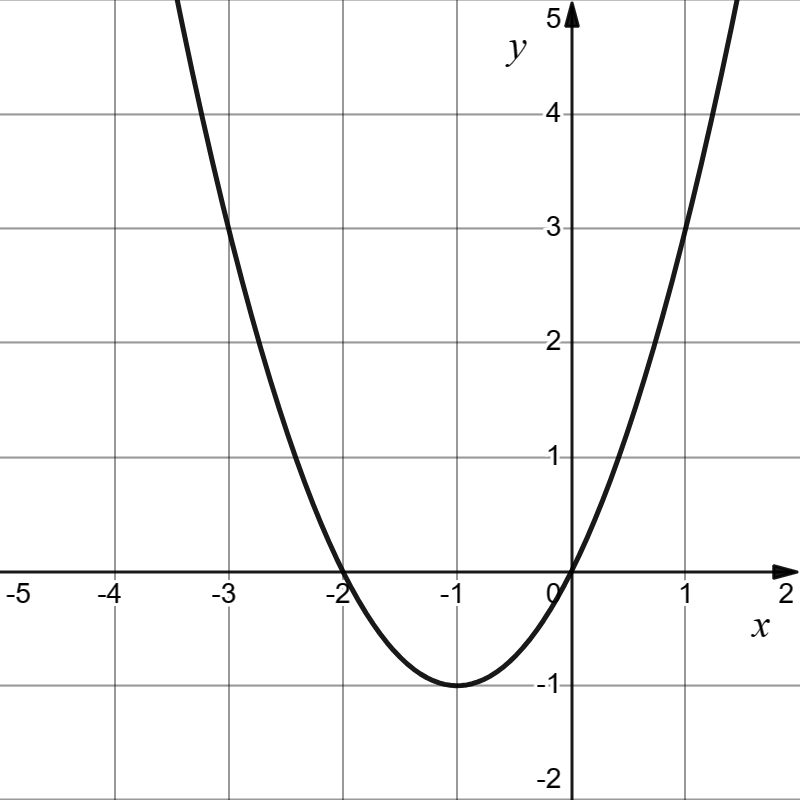
\includegraphics[scale=0.25]{figs/f(x)=x^2+2x.png}
    % \end{center}
  \end{multicols}
\end{example}
\vspace*{-12\baselineskip}

\newpage

\begin{definition}
  A function is a \textbf{one-to-one function} if each output value corresponds to exactly one input value.
\end{definition}

\begin{example}
  Is the area of a circle a function of its radius? If yes, is the function one-to-one?
\end{example}

\begin{howto}
  A graph is a function if very vertical line crosses the graph at most once. This method is known as the \textbf{vertical line test}.

A function is an one-to-one if very horizontal line crosses the graph at most once. This method is known as the \textbf{horizontal line test}.
\end{howto}

\begin{example}
  Determine if the graph defines a function. If so, is it a one-to-one function?
  \begin{center}
  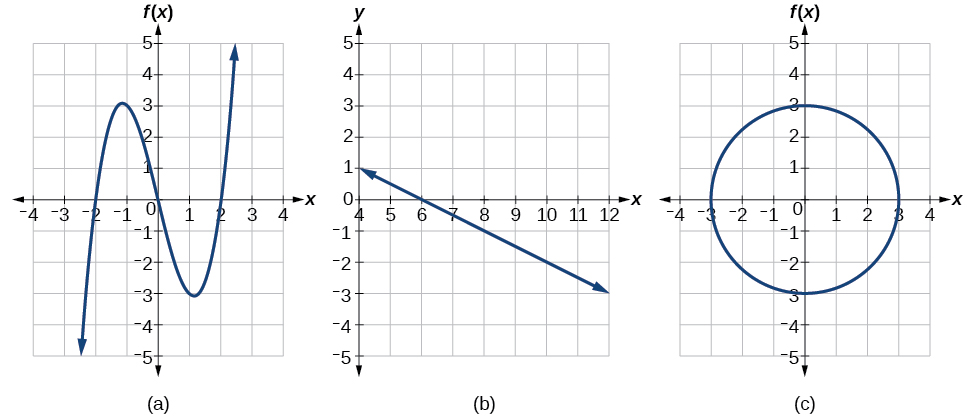
\includegraphics[width=0.8\textwidth]{figs/cubic-line-circle.jpg}
  \end{center}
\end{example}

\newpage
\section*{Exercises}

\begin{exercise}
  Consider the function $f(x)=2x^2+x-3$. Find the values of the following expressions.

\begin{enumerate}[fourcol]
  \item \(f(-1)\)
  \item \(f(a)\)
  \item \(f(a+h)\)
  \item \(\dfrac{f(a+h)-f(a)}{h}\)
\end{enumerate}
\end{exercise}
\vspace*{2\baselineskip}

\begin{exercise}
  For the function $f(x)=-4x+5$, evaluate and simplify the difference quotient $\dfrac{f(x+h)-f(x)}{h}$.
\end{exercise}
\vspace*{2\baselineskip}

\begin{exercise}
  Consider the function $f(x)=-x^2-4x$. Find all $x$ values such that $f(x)=3$.
\end{exercise}

\newpage

\begin{exercise}
  Express the relationship defined by the function $3x-2y-6=0$ as a function $y=l(x)$.
\end{exercise}

\begin{exercise}
  If \(8x-y^3=0\), express \(y\) as a function of \(x\).

  Is $y$ a one-to-one function of $x$?
\end{exercise}


\begin{exercise}
  Consider the function $f(x)$ defined by a graph below.

  \begin{multicols}{2}
    \begin{enumerate}
      \item Find $f(1)$. 
      \item Find all $x$ such that $f(x)=3$.
    \end{enumerate}
    \vfill\mbox{}

    \columnbreak
   
    \begin{tikzpicture}
      \begin{axis}[
      width=0.6\textwidth,
      xmin=-2,
      xmax=5,
      ymin=-2,
      ymax=5,
      xtick={-10,-9,...,10},
      ytick={-10,-9,...,10},
      ]
      \addplot[blue, line width=1.5pt, smooth,samples=100] {-x^2+2*x+2} node[pos=0.7, right] {$y=f(x)$};
      \end{axis}
      \end{tikzpicture}

    % \begin{center}
    %   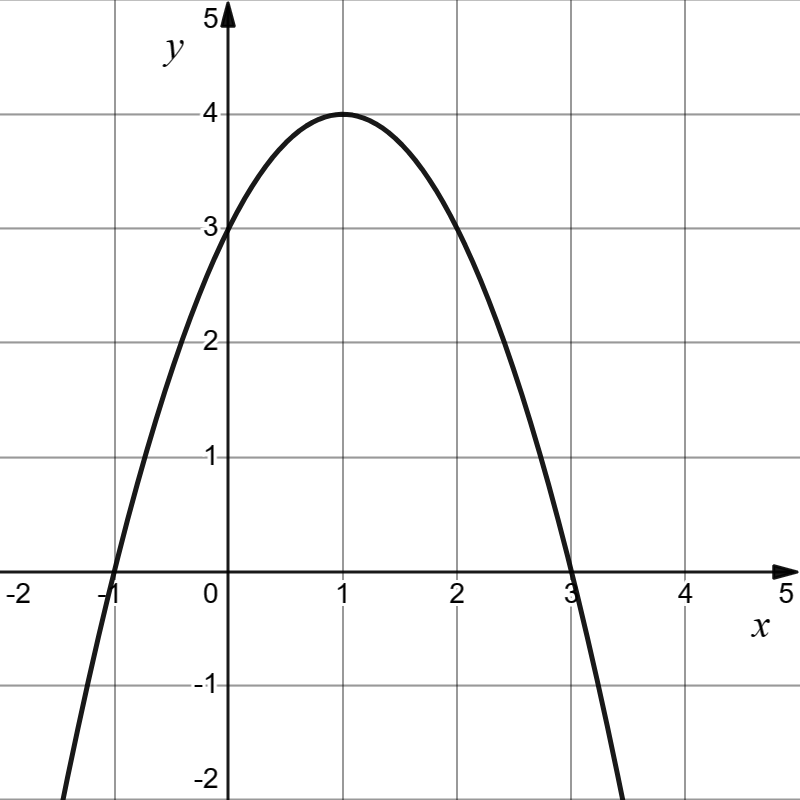
\includegraphics[scale=0.3]{figs/f(x)=-x^2+2x+2.png}
    % \end{center}
  \end{multicols}
\end{exercise}
\vspace{-10\baselineskip}


\newpage
\thispagestyle{fancy}

\section{Domains and Ranges}
\begin{howto}
The domain of a function $f$ consists of possible input values $x$. Or equivalently, the domain consists of all $x$ values except those that will make the function is undefined.

The range of a function $f$ consists of all possible output values $y$. Equivalently, the range consists of $y$ value such that equation $y=f(x)$ has a solution $x$. 
\end{howto}

\begin{example}
  Find the domain of the function $$f(x)=\dfrac{x+1}{2-x}.$$
\end{example}

\begin{example}
  Find the domain of the function
$$
f(x)=\sqrt{7-x}.
$$
\end{example}

\begin{definition}
  \textbf{Set-builder notation} is a method of specifying a set of elements that satisfy a certain condition. It takes the form $\{x|\text{ statement about x}\}$ which is read as, ``the set of all x such that the statement about x is true."
  
  \textbf{Interval notation} is a way of describing sets that include all real numbers between a lower limit that may or may not be included and an upper limit that may or may not be included. The endpoint values are listed between brackets or parentheses. A square bracket indicates inclusion in the set, and a parenthesis indicates exclusion from the set.
\end{definition}

\newpage

\begin{example}
  Find the domain of the function $f(x)=\dfrac{\sqrt{x+2}}{x-1}$. Write your answer in set-builder notation and interval notation.
\end{example}


\begin{example}
  Find the domain and range of the function $f$ whose graph is shown in Figure.

  \begin{tikzpicture}
    \begin{axis}[
    width=0.7\textwidth,
    xmin=-4,
    xmax=4,
    ymin=-2,
    ymax=10,
    xtick={-10,-9,...,10},
    ytick={-10,-9,...,10},
    ]
    \addplot[blue, line width=1.5pt, smooth,samples=100,domain=-3:2] {(-x^3+3*x)/2} node[pos=0.15,right] {$y=f(x)$};
    \addplot[mark=*, mark size=3pt] coordinates {(-3,9)};
    \addplot[mark=o, mark size=3pt] coordinates {(2,-1)};
    \end{axis}
    \end{tikzpicture}

  % 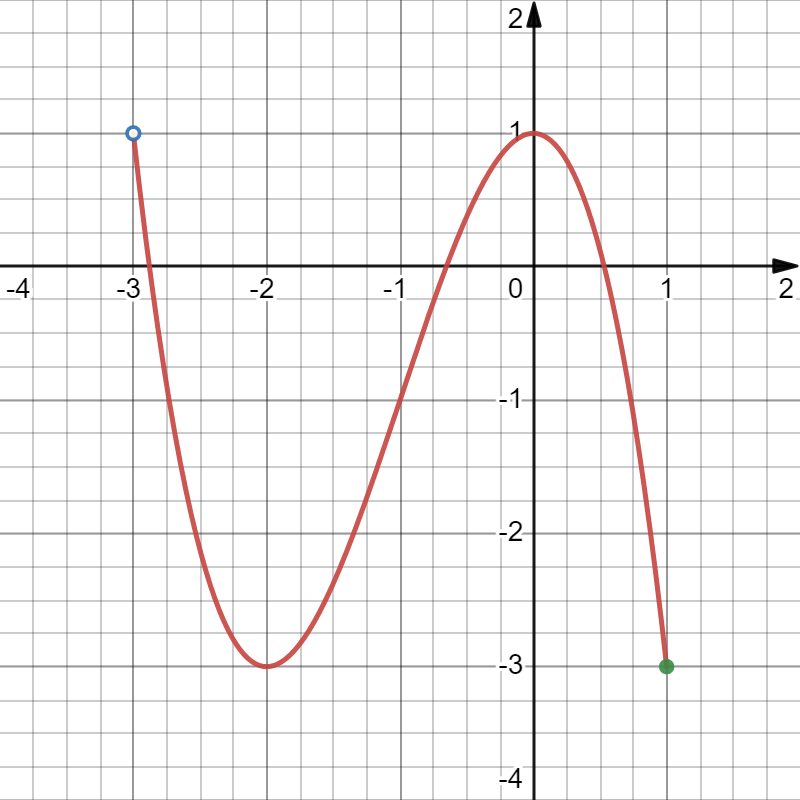
\includegraphics[width=0.6\textwidth]{figs/FindDomainRangeCubic.png}
\end{example}
\vspace*{-8\baselineskip}

\begin{example}
  Find the domain and range of the function
  $$f(x)=\frac{2}{x+3}.$$
\end{example}

\newpage

\begin{example}
  Find the domain and range of the function
  $$f(x)=3\sqrt{x+2}.$$
\end{example}


\begin{example}
  Consider the piecewise function
  $$
  f(x)=\begin{cases}
    2x-3 & \text{if}\quad x\le -1\\
    -x^2 & \text{if}\quad -1<x< 1\\
    -2x+4 & \text{if}\quad 1\le x.
  \end{cases}
  $$
  \begin{enumerate}[threecol]
    \item Sketch the graph
    \item Find $f(-4)$
    \item Find $f(2)$
  \end{enumerate}
\end{example}

\newpage

\section*{Exercises}

\begin{exercise}
  Find the domain of the function\\
  \begin{enumerate*}
    \item  $f(x)=\dfrac{1+4x}{2x-1}$ 
    \item  $f(x)=\sqrt{5+2x}$
    \item  $f(x)=\dfrac{\sqrt{x+1}}{x-1}$
    \item $f(x)=\dfrac{x-2}{x^2+7x-44}$
  \end{enumerate*}
\end{exercise}
\vspace*{\stretch{5}}

\begin{exercise}
  Estimate the domain and range for the function defined by the graph. Write your answer in interval notation.\\
  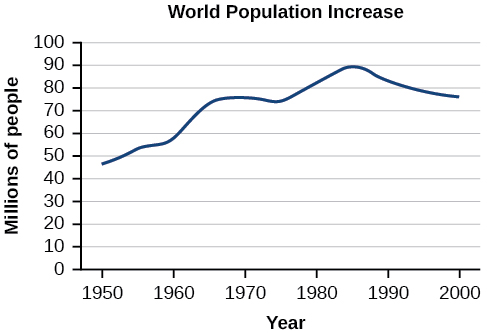
\includegraphics[width=0.6\textwidth]{figs/CNX_Precalc_Figure_01_02_010.jpg}
\end{exercise}
\vspace*{-5\baselineskip}

\newpage

\begin{exercise}
  Find the domain and range of each of the following functions. Write your answer in set-builder notation and interval notation.
  \begin{enumerate}[twocol]
    \item $f(x)=\frac{3}{x-2}$
    \item $f(x)=-2\sqrt{x+4}$
  \end{enumerate}
\end{exercise}

\begin{exercise}
  Consider the piecewise function
  $$f(x)=\begin{cases}
    -2x+5 & \text{if}\quad x< -2\\
    x^2-1 & \text{if}\quad -2\le x\le 2\\
    2x-3 & \text{if}\quad 2< x.
  \end{cases}$$
  \begin{enumerate}[threecol]
    \item Sketch the graph
    \item Find $f(-4)$
    \item Find $f(2)$
  \end{enumerate}
\end{exercise}

\newpage

\section{Rates of Change and Behavior of Graphs}

\begin{definition}[Rate of Change]
  The average rate of change of $f$ over an interval $[a,b]$ is defined as
  $$\text{Average Rate Of Change}=\dfrac{f(b)-f(a)}{b-a}.$$
  The average rate of change is the same as the slope of secant line passing through $(a, f(a))$ and $(b, f(b))$.
  
  By taking $x=a$ and $h=b-a$, the average of rate of change is the same the difference quotient of a function $f$ which is defined as
  $$\text{Difference Quotient}=\dfrac{f(x+h)-f(x)}{h}.$$
\end{definition}

\begin{example}
  After picking up a friend who lives 10 miles away, Anna records her distance from home over time. The values are shown in Table. Find her average speed over the first 6 hours.
\begin{center}
  \begin{tabular}{l*{8}{c}}
    $t$ (hours) & 0 & 1 & 2 & 3 & 4 & 5 & 6 & 7\\
    $D(t)$ (miles) & 10 & 55 & 90 & 153 & 214 & 240 & 292 & 300
  \end{tabular}
\end{center}
\end{example}

\begin{example}
  Find the average rate of change of $f(x)=x^2-\dfrac{1}{x}$ over the interval $[2, 4]$.
\end{example}

\newpage

\begin{example}
  Find the average rate of change of  $g(t)=t^2+3t+1$ on the interval  $[0,a]$. The answer will be an expression involving $a$.
\end{example}



\begin{definition}[Increasing and Decreasing]
  A function $f$ is \textbf{increasing} over an interval $(a, b)$ if $f(x_2)>f(x_1)$ for any $x_1<x_2$ in $(a, b)$. Equivalently, $f$ is increasing over $(a, b)$ if  the average rate of change is positive over any subinterval $(x_1, x_2)$ of $(a, b)$.
  
  A function $f$ is \textbf{decreasing} over an interval $(a, b)$ if $f(x_2)<f(x_1)$ for any $x_1<x_2$ in $(a, b)$. Equivalently, $f$ is decreasing over $(a, b)$ if  the average rate of change is negative over any subinterval $(x_1, x_2)$ of $(a, b)$.

  \begin{center}
    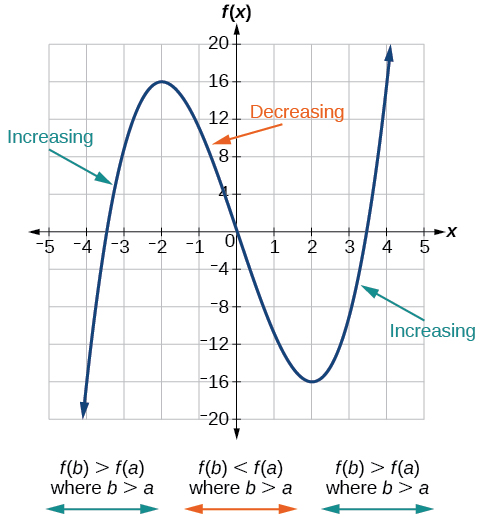
\includegraphics[width=0.6\textwidth]{figs/CNX_Precalc_Figure_01_03_004.jpg}
  \end{center}
\end{definition}

\newpage

\begin{definition}[Local Maxima and Minima]
  A function \(f\) has a \textbf{local maximum} at \(x=c\) if $f(c)\ge f(x)$ for any $x$ in a small interval containing $c$. A small interval containing $c$ is also known as a small \text{neighborhood} of $c$.

  A function \(f\) has a \textbf{local minimum} at \(x=c\) if $f(c)\le f(x)$ for any $x$ in a small interval containing $c$.
\end{definition}

\begin{howto}
  A function $f$ has a local maximum at $x=c$ if it changes from increasing to decreasing at $c$ in a neighborhood of $c$.
  
  A function $f$ has a local minimum at $x=c$ if it changes from decreasing to increasing at $c$ in a neighborhood of $c$.
\end{howto}



\begin{example}
  Find the interval of increasing and the interval of decreasing, and the local maxima and local minima of the function $f$ defined by the following graph.

  \begin{tikzpicture}
    \begin{axis}[
    xmin=-3,
    xmax=3,
    ymin=-3,
    ymax=3,
    xtick={-10,-9,...,10},
    ytick={-10,-9,...,10},
    ]
    \addplot[latex-latex, blue, line width=1.5pt, smooth,samples=100,domain=-2:2] {x^3-3*x} node[pos=0.4, right] {$y=f(x)$};
    \end{axis}
  \end{tikzpicture}

  % \begin{center}
  %   \raggedright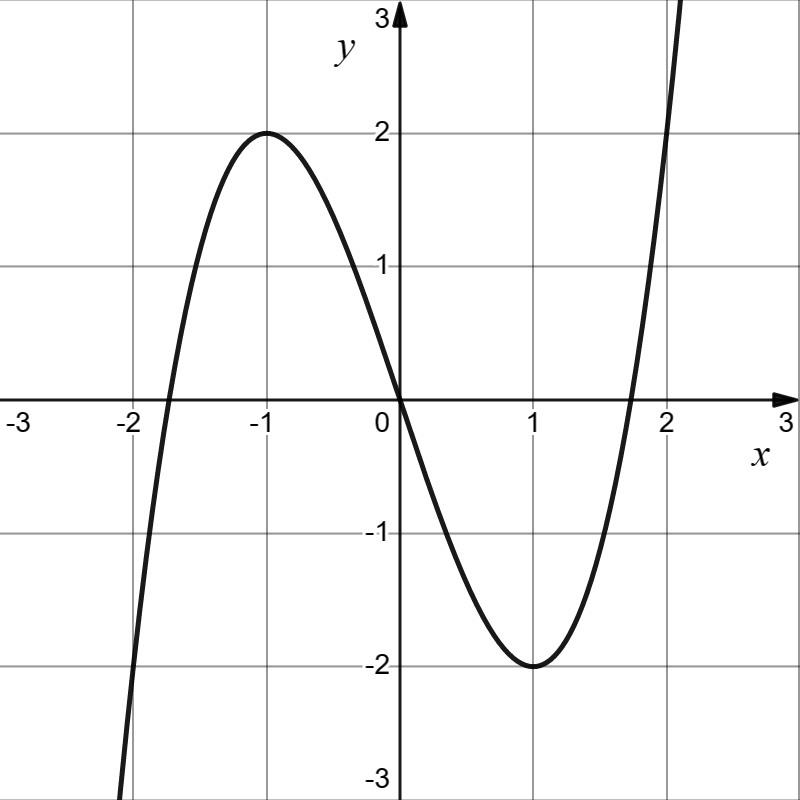
\includegraphics[width=0.5\textwidth]{figs/x^3-3x.png}
  % \end{center}
\end{example}

% \vspace*{-0.1\textheight}
% \newpage

\begin{definition}[Absolute Maxima and Minima]
  The \textbf{absolute maximum} of $f$ at \(x=c\) is \(f(c)\) where \(f(c)\ge f(x)\) for all \(x\) in the domain of \(f\).
  
  The \textbf{absolute minimum} of $f$ at \(x=c\) is \(f(c)\) where \(f(c)\le f(x)\) for all \(x\) in the domain of \(f\).
\end{definition}

\begin{example}
  Finding the absolute maximum and minimum of the function $f$ defined by the following graph.
  
  \begin{tikzpicture}
    \begin{axis}[
    % width=0.6\textwidth,
    xmin=-4,
    xmax=3,
    ymin=-3,
    ymax=4,
    xtick={-10,-9,...,10},
    ytick={-10,-9,...,10},
    ]
    \addplot[blue, line width=1.5pt, smooth,samples=100,domain=-3:1.5] {(-x^3+3*x-6)/4} node[pos=0.3, right] {$y=f(x)$};
    \addplot[mark=*, mark size=3pt] coordinates {(-3,3)};
    \addplot[mark=o, mark size=3pt] coordinates {(1.5,-1.21875)};
    \end{axis}
    \end{tikzpicture}

  % \begin{center}
  %   \raggedright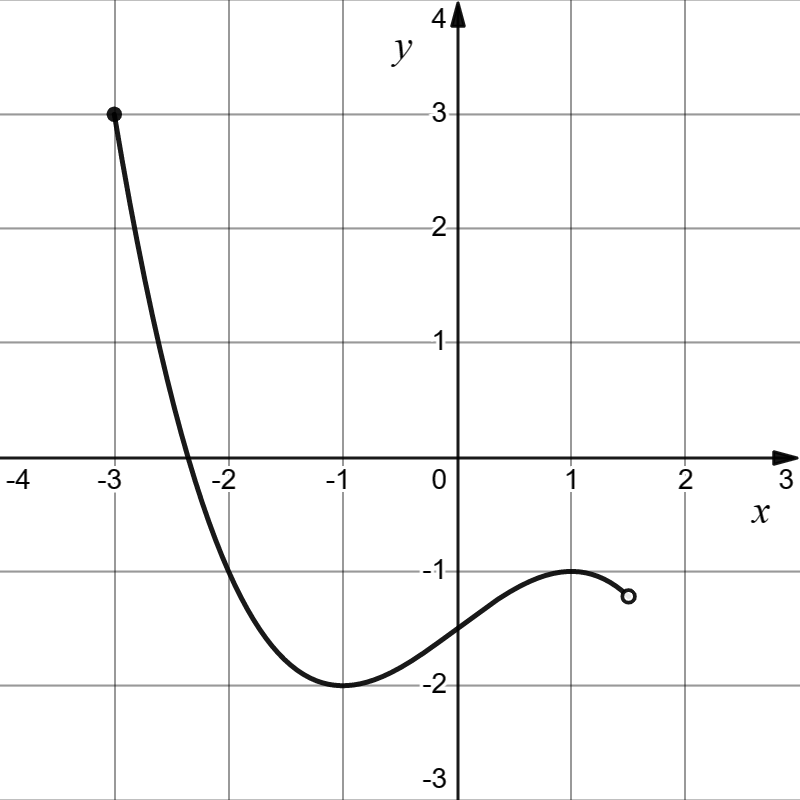
\includegraphics[width=0.5\textwidth]{figs/(-x^3+3x-6)divby4.png}
  % \end{center}
\end{example}

\newpage
\section*{Exercises}

\begin{exercise}
  The electrostatic force  $F$, measured in newtons, between two charged particles can be related to the distance between the particles  $d$, in centimeters, by the formula  $F(d)=\dfrac{2}{d^2}$. Find the average rate of change of force if the distance between the particles is increased from 2 cm to 6 cm.
\end{exercise}

\begin{exercise}
  Find the average rate of change of $f(x)=x^2+2x-8$ on the interval $[5,a]$.
\end{exercise}

\begin{exercise}
  Find the interval of increasing and the interval of decreasing, and the local maxima and local minima of the function $f$ defined by the following graph.

  \begin{tikzpicture}
    \begin{axis}[
    xmin=-3,
    xmax=8,
    ymin=-8,
    ymax=3,
    xtick={-10,-9,...,10},
    ytick={-10,-9,...,10},
    ]
    \addplot[latex-latex, blue, line width=1.5pt, smooth,samples=100,domain=-2.8:7.8] {(x^3-6*x^2-15*x+16)/12} node[pos=0.4, right] {$y=f(x)$};
    \end{axis}
    \end{tikzpicture}
  % \begin{center}
  %   \raggedright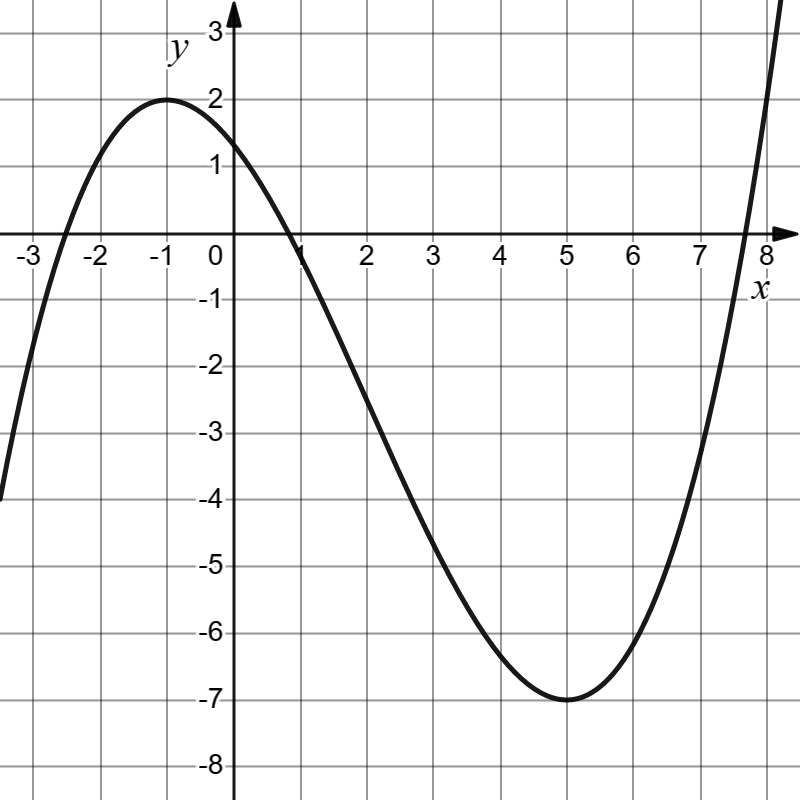
\includegraphics[width=0.5\textwidth]{figs/(xcube-6xsq-15x+16)divby12.png}
  % \end{center}
\end{exercise}
\vspace{-12\baselineskip}

\newpage

\begin{exercise}
  Finding the absolute maximum and minimum of the function $f$ defined by the following graph.
  
  \begin{tikzpicture}
    \begin{axis}[
    width=0.6\textwidth,
    xmin=-3,
    xmax=4,
    ymin=-3,
    ymax=4,
    xtick={-10,-9,...,10},
    ytick={-10,-9,...,10},
    ]
    \addplot[blue, line width=1.5pt, smooth,samples=100,domain=-1.5:3] {(-x^3+3*x+10)/4} node[pos=0.6, right] {$y=f(x)$};
    \addplot[mark=*, mark size=3pt] coordinates {(3,-2)};
    \addplot[mark=o, mark size=3pt] coordinates {(-1.5,2.25)};
    \end{axis}
    \end{tikzpicture}

  % \begin{center}
  %   \raggedright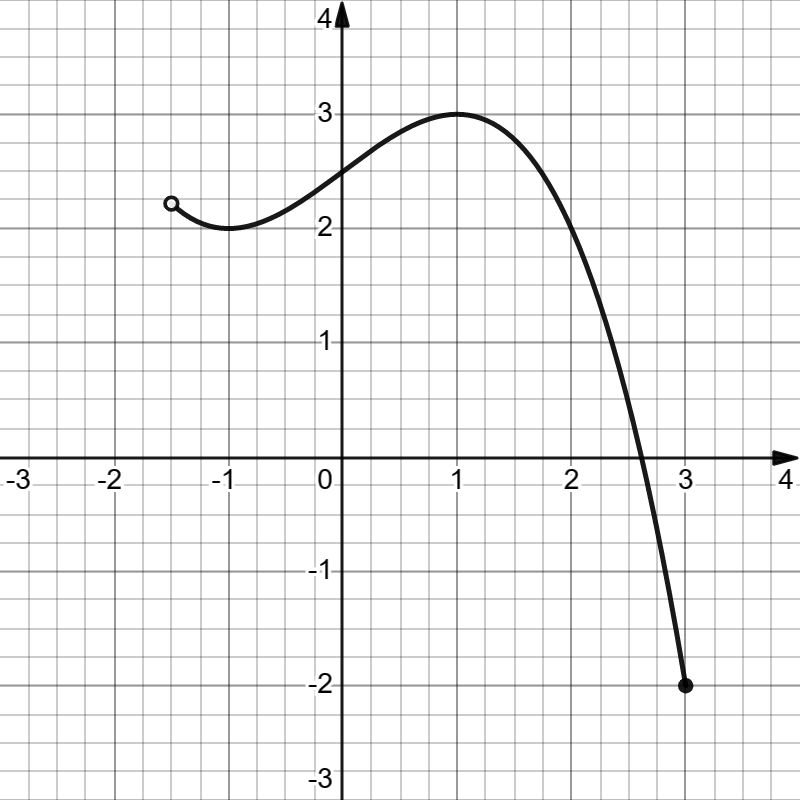
\includegraphics[width=0.5\textwidth]{figs/(-x^3+3x+10)divby4.png}
  % \end{center}
\end{exercise}
\vspace*{-0.4\textheight}

\begin{exercise}
  Find the interval of increasing and the interval of decreasing, and the local maxima and local minima of the function $f(x)=x^3-6x^2-15x+20$ using its graph.
  %f\left(x\right)=2x^{3}-3x^{2}-12x+7
\end{exercise}

\newpage

\section{Combination and Composition of Functions}

\begin{definition}[Algebraic Operations of Functions]
  Let \(f\) and \(g\) be two functions with domains $A$ and $B$ respectively. We define the linear combination, product, and quotient functions as follows.
  \begin{center}
    \begin{tabular}{rcl}
      Linear combination: & $(af+bg)(x)=af(x)+bg(x)$ & with the domain $A\cap B$.\\
      Product: & $(fg)(x)=f(x)g(x)$ & with the domain: $A\cap B$.\\
      Quotient: & $\left(\dfrac{f}{g}\right)(x)=\dfrac{f(x)}{g(x)}$ & with the domain: $A\cap B\cap \{x\mid g(x)\neq 0\}$.
    \end{tabular}
  \end{center}
  
\end{definition}

\begin{example}
  Consider the functions \(f(x)=x-1\) and \(g(x)=x^2-1\). Find and simplify the functions \((g-f)(x)\) and \(\left(\dfrac{g}{f}\right)(x)\), and their domains.
\end{example}

\begin{definition}[Composition of functions]
  Let \(f\) and \(g\) be two functions with domains $A$ and $B$ respectively. The \textbf{composite function} $f\circ g$ (also called the
  composition of $f$ and $g$) is defined as
  \[(f\circ g)(x)=f(g(x))\qquad \text{with the domain:}\quad B\cap \{x\mid g(x)\in A\}.\]
\noindent
  We read the left-hand side as ``\(f\) composed with \(g\) at \(x\),'' and the right-hand side as ``\(f\) of \(g\) of \(x\).''
\end{definition}

\begin{example}
  Consider the functions \(f(x)=\sqrt{x-2}\) and \(g(x)=x^2+1\). 
  \begin{enumerate}
    \item Find and simplify the functions \((f\circ g)(x)\) and \((g\circ f))(x)\).  Are they the same function?
    \item Find the domains of $f\circ g$ and $g\circ f$. Are they the same?
  \end{enumerate}
\end{example}

\newpage

\begin{example}
  Consider $f(t)=t^2-4t$ and $h(x)=\sqrt{x+3}$. Evaluate\\ 
  \begin{enumerate*}
    \item $\dfrac{f(1)}{g(1)}$
    \item $h(f(-1))$
    \item $(f\circ h)(-1))$
    \item $(f-h)(-1)$
  \end{enumerate*}
\end{example}

\vspace*{2\baselineskip}

\begin{example}
  Using the graphs to evaluate the given functions.
  \begin{multicols}{2}
    \begin{enumerate}
      \item $(f+g)(1)$
      \item $(fg)(1)$
      \item $\left(\dfrac{f}{g}\right)(1)$
      \item $(g\circ f)(-3)$
      \item $f(g(0))$
      % \vfill\mbox{}
    \end{enumerate}
    \columnbreak
    \begin{tikzpicture}
      \begin{axis}[
        width=0.65\textwidth,
      xmin=-4,
      xmax=5,
      ymin=-4,
      ymax=5,
      xtick={-10,-9,...,10},
      ytick={-10,-9,...,10},]
      \addplot[blue, line width=1.5pt, smooth,samples=100] {-(x-2)^2+3} node[pos=0.85, right] {$y=g(x)$};
      \addplot[red, line width=1.5pt, smooth,samples=100] {(x+1)^2-2} node[pos=0.2, right] {$y=f(x)$};
      \end{axis}
      \end{tikzpicture}

    % 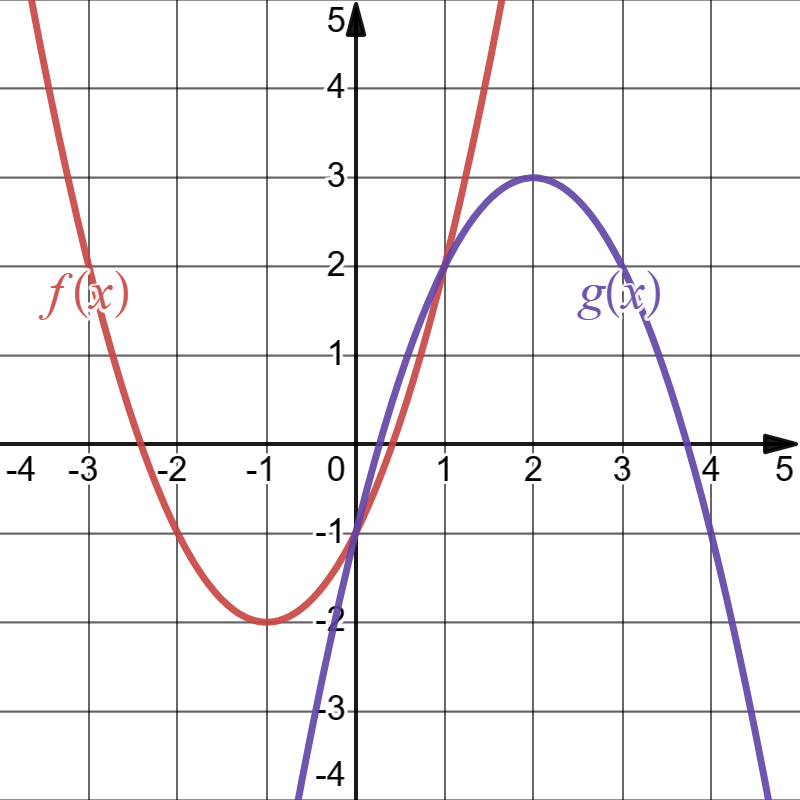
\includegraphics[width=0.45\textwidth]{figs/twoquadratics.png}
  \end{multicols}
\end{example}
\vspace*{-0.1\textheight}

\begin{example}
  Consider the function $h(x)=\sqrt{x^2+1}$. Find two functions $f$ and $g$ so that $h(x)=f(g(x))$.
\end{example}

\newpage

\section*{Exercises}

\begin{exercise}
  Consider the functions \(f(x)=x^2-1\) and \(g(x)=x+1\). 
  \begin{enumerate}
    \item Find the function \((f-g)(x)\) and its domain.
    \item Find the function \((fg)(x)\) and its domain.
    \item Find \(\left(\dfrac{f}{g}\right)(x)\) and its domain.
    \item Find \((2f-3g)(1)\).
    \item Find \(2fg-\left(\dfrac{3g}{f}\right)(1)\).
  \end{enumerate}
\end{exercise}

\begin{exercise}
  Consider the functions $f(x)=\dfrac{1}{x-2}$ and $g(x)=\sqrt{x+4}$.

\begin{enumerate}
  \item Find $f\circ g$ and its domain.
  \item Find $(g\circ f)(3)$.
\end{enumerate}
\end{exercise}

\newpage

\begin{exercise}
    Using the graphs to evaluate the given functions.
    \begin{multicols}{2}
      \begin{enumerate}
        \item $(f-g)(1)$
        \item $(fg)(0)$
        \item $\left(\dfrac{f}{g}\right)(0)$
        \item $(f\circ g)(2)$
        \item $g(f(0))$
      \end{enumerate}

      \columnbreak

      \begin{tikzpicture}
        \begin{axis}[
          width=0.65\textwidth,
        xmin=-3,
        xmax=4,
        ymin=-3,
        ymax=4,
        xtick={-10,-9,...,10},
        ytick={-10,-9,...,10},]
        \addplot[blue, line width=1.5pt, smooth,samples=100] {-2*x^2+3} node[pos=0.55, above right] {$y=f(x)$};
        \addplot[red, line width=1.5pt, smooth,samples=100] {(x-1)^2-2} node[pos=0.6, above left] {$y=g(x)$};
        \end{axis}
        \end{tikzpicture}

      % 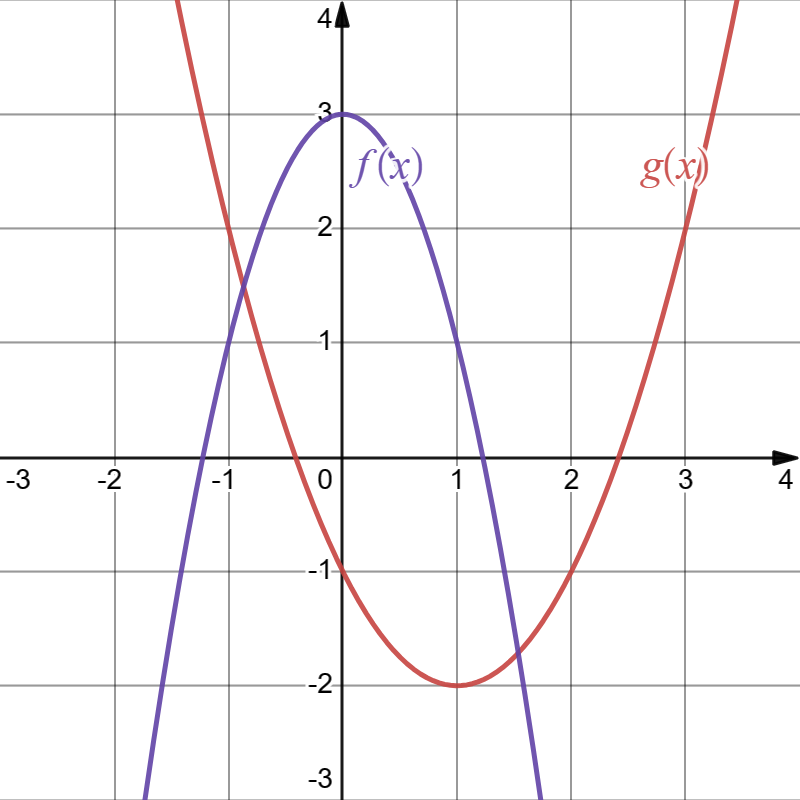
\includegraphics[width=0.5\textwidth]{figs/two-quadratics-exr.png}
    \end{multicols}
\end{exercise}
\vspace*{-0.2\textheight}

\begin{exercise}
  Consider the function $h(x)=\sqrt[3]{2x-1}$. Find two functions $f$ and $g$ so that $h(x)=f(g(x))$.
\end{exercise}

\newpage

\section{Transformations}

\begin{definition}
  Given a function \(y=f(x)\), the function \(y=f(x)+k\), where \(k\) is a constant, is a \textbf{vertical shift} of the function \(f\). 
\end{definition}

\begin{howto}
  Suppose $k$ is positive. 
\begin{itemize}
  \item To graph $y=f(x) {\color{red} +}k$, shift the graph of $y=f(x)$ {\color{red}upward} $k$ units. 
  \item To graph $y=f(x) {\color{blue} -}k$, shift the graph of $y=f(x)$ {\color{blue}downward} $k$ units. 
\end{itemize}
\end{howto}

\begin{example}
  Consider the functions $f(x)=x^2$, $g(x)=x^2-1$ and $h(x)=x^2+2$.
  \begin{enumerate}
    \item Describe how to get the graph of $g$ from the graph of $f$.
    \item Describe how to get the graph of $h$ from the graph of $f$.
    \item Describe how to get the graph of $f$ from the graph of $h$.
    \item Describe how to get the graph of $h$ from the graph of $g$.
  \end{enumerate}
\end{example}

% \begin{example}
%   A function $y=f(x)$ is given in the table below. Create a table for the function $g(x)=f(x)-3$.
%   \begin{center}
%     \begin{tabular}{c*{4}{c}}
%      $x$ & 1 & 2 & 5 & 10\\
%      $f(x)$ & 0 & 1 & 2 & 3
%     \end{tabular}
%   \end{center}
% \end{example}



\begin{definition}
  Given a function \(y=f(x)\), the function \(y=f(x-h)\), where \(h\) is a constant, is a \textbf{horizontal shift} of the function \(f\). 
  \end{definition}

\begin{howto}
  Suppose $h$ is positive. 
\begin{itemize}
  \item To graph $y=f(x {\color{red} -} h)$, shift the graph of $y=f(x)$ to the {\color{red} right} $h$ units. 
  \item To graph $y=f(x {\color{blue} +} h)$, shift the graph of $y=f(x)$ to the {\color{blue} left} $h$ units. 
\end{itemize}
\end{howto}

\begin{example}
  Consider the functions $f(x)=x^2$, $g(x)=(x+1)^2$ and $h(x)=(x-2)^2$.
  \begin{enumerate}
    \item Describe how to get the graph of $g$ from the graph of $f$.
    % \vspace*{3\baselineskip}
    \item Describe how to get the graph of $h$ from the graph of $f$.
    % \vspace*{3\baselineskip}
    \item Describe how to get the graph of $f$ from the graph of $h$.
    % \vspace*{3\baselineskip}
    \item Describe how to get the graph of $h$ from the graph of $g$.
    % \vspace*{3\baselineskip}
  \end{enumerate}
\end{example}

\newpage

\begin{example}
  Sketch the graph of \(f(x)=|x|\). Then use the graph to sketch the graph of \(h(x)=f(x+2)-1\). 
\end{example}

\begin{example}
  The function $y=g(x)$ shown in the picture is a shift of the square root function $y=\sqrt{x}$. Find $g(x)$.\\

  \begin{tikzpicture}[scale=1.2]
    \begin{axis}[
    xmin=-2,
    xmax=2,
    ymin=-2,
    ymax=2,
    xtick={-5,-4,...,5},
    ytick={-5,-4,...,5},]
    \addplot[blue, line width=1.5pt, smooth,samples=100,domain=-1:2] {sqrt(x+1)-1} node[pos=0.7, above left] {$y=g(x)$};
    \end{axis}
    \end{tikzpicture}
  % \begin{center}
  %   \raggedright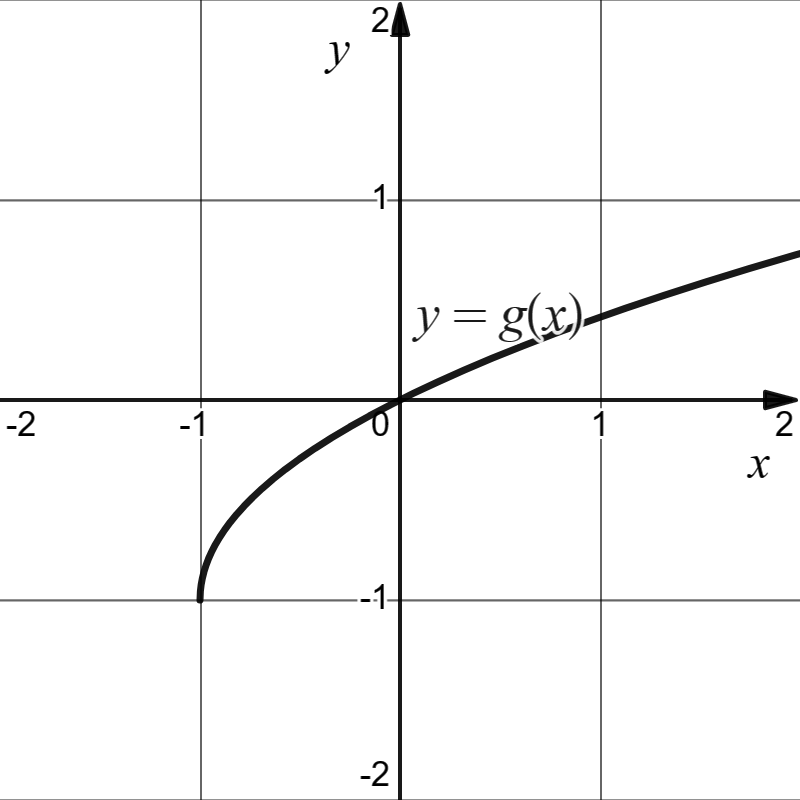
\includegraphics[width=0.5\textwidth]{figs/shiftsqrtexm.png}
  % \end{center}
\end{example}
\vspace*{-0.4\textheight}

\newpage

\begin{definition}
  Given a function \(y=f(x)\), the function \(g(x)=-f(x)\) is a \textbf{vertical reflection} of the function \(y=f(x)\), or a reflection about the $x$-axis;
the function \(g(x)=f(-x)\) is a \textbf{horizontal reflection} of the function \(y=f(x)\) or a reflection about the $y$-axis.
\end{definition}

\begin{example}
  Reflect the graph of \(f(x)=|x-1|\)\\
  \begin{enumerate*}
    \item first vertically,
    \item then horizontally.\hfill\mbox{}
  \end{enumerate*}

Denote the new function by $y=g(x)$. Find $g(x)$.
\end{example}

\begin{example}
  A common model for learning has an equation similar to \(k(t)=-2^{-t}+1\), where \(k\) is the percentage of mastery that can be achieved after \(t\) practice sessions, and $t>0$. The function $k$ is a transformation of a part of the function \(f(t)=2^t\) shown below. Sketch the graph of \(k(t)\).\\
  \begin{tikzpicture}
    \begin{axis}[
      width=0.75\textwidth,
    xmin=-5,
    xmax=5,
    ymin=-5,
    ymax=5,
    xlabel={$t$},
    ylabel={$k(t)$},
    xtick={-10,-9,...,10},
    ytick={-10,-9,...,10},]
    \addplot[blue, line width=1.5pt, smooth,samples=100,domain=-5:3] {2^x} node[pos=0.9, right] {$y=f(x)$};
    \addplot[mark=*] coordinates {(-2, 0.25)} node[above left] {$(-2,\frac14)$};
    \addplot[mark=*] coordinates {(-1, 0.5)} node[above left] {$(-1,\frac12)$};
    \addplot[mark=*] coordinates {(0, 1)};
    \addplot[mark=*] coordinates {(1, 2)} node[below right] {$(1,2)$};
    \end{axis}
    \end{tikzpicture}

% 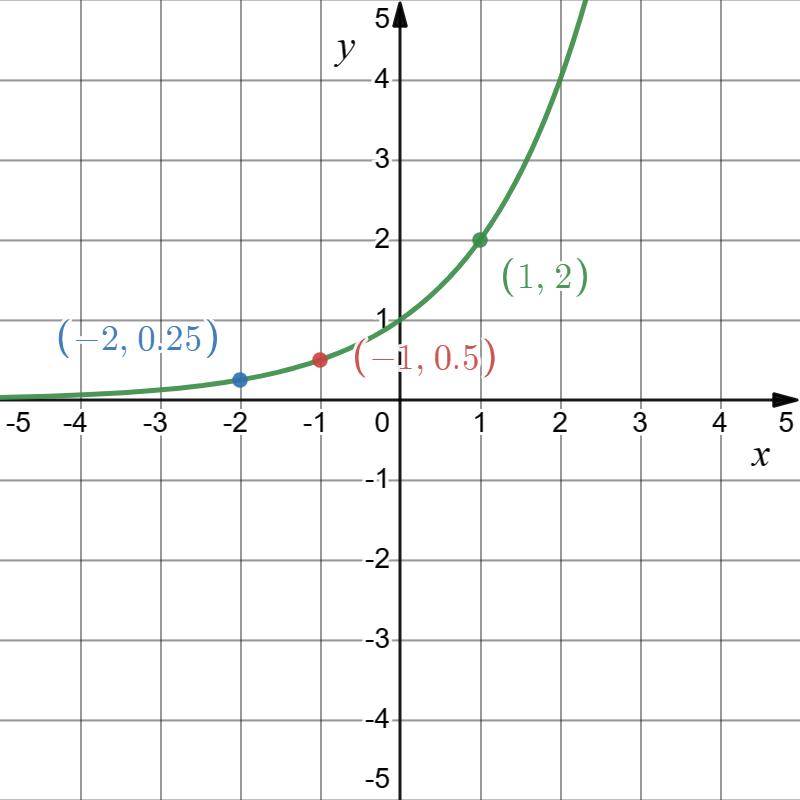
\includegraphics[width=0.5\textwidth]{figs/learningmodel.png}
\end{example}
\vspace*{-0.3\textheight}

\newpage

\begin{definition}
  A function is called an \textbf{even function} if $f(-x)=f(x)$ for $x$ in the domain of $f$.
  
  A function is called an \textbf{odd function} if $f(-x)=-f(x)$ for $x$ in the domain of $f$.
\end{definition}

\begin{remark}
  The graph of an even function is symmetric about $y$-axis.

  The graph of an odd function is symmetric about the origin. This symmetry is known as a rotation symmetry.
\end{remark}

\begin{example}
  Group the functions according to even, odd, or other.\\
  \begin{enumerate*}
    \item $f(x)=x^2-1$
    \item $g(x)=|x-1|$
    \item $h(x)=x^3-2x$
    \item $k(x)=\dfrac{1}{x^2}$.
  \end{enumerate*}
\end{example}

\begin{definition}
  Let $c$ be a positive number.
  The function $g(x)=cf(x)$ is called a \textbf{vertical stretch} or \textbf{vertical compression} of $y=f(x)$ by a factor of $c$ if $c>1$ or $0<c<1$ respectively.
\end{definition}
\begin{remark}
  If $a<0$, then $g(x)=cf(x)$ is a combination of a vertical stretch or compression with a vertical reflection.
\end{remark}

\begin{example}
  The point $(9, -15)$ is on the graph of $y=f(x)$. Find a point on the graph of $g(x)=\dfrac{1}{3}f(x)$.
\end{example}
\vspace*{-0.3\textheight}

\newpage
\begin{example}
  The function $y=g(x)$ given in the following graph can be obtained from $f(x)=x^2$ by a combination of shifting, reflecting, and stretching. Describe the transformation and find an equation of $g$.\\
  \begin{tikzpicture}[scale=1.2]
    \begin{axis}[
    xmin=-3,
    xmax=5,
    ymin=-3,
    ymax=5,
    xtick={-10,-9,...,10},
    ytick={-6,-5,...,6},]
    \addplot[blue, line width=1.5pt, smooth,samples=100,domain=-1:3] {-2*(x-1)^2+4} node[pos=0.5, right] {$y=g(x)$};
    \end{axis}
    \end{tikzpicture}

  % 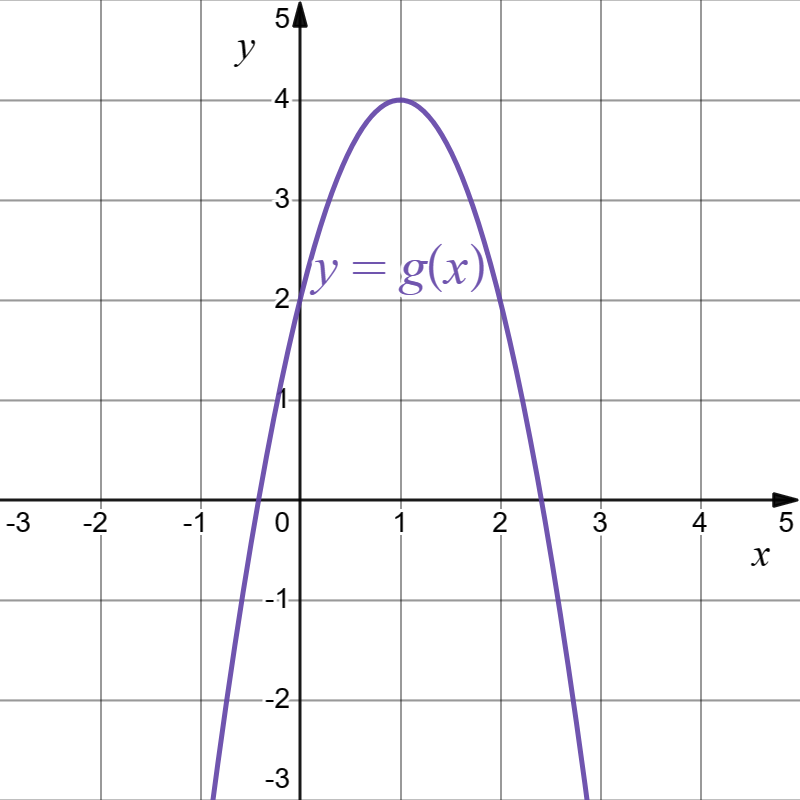
\includegraphics[width=0.5\textwidth]{figs/transformationquadratic.png}
\end{example}
\vspace*{-0.1\textheight}

\begin{definition}
  Let $c$ be a positive number.
  The function $g(x)=f(cx)$ is called a \textbf{horizontal stretch} or \textbf{horizontal compression} of $y=f(x)$ by a factor of $\dfrac{1}{c}$ if $0<c<1$ or $c>1$ respectively.
\end{definition}
\begin{remark}
  If $c<0$, then $g(x)=f(cx)$ is a combination of a horizontal stretch or compression with a horizontal reflection.
\end{remark}
\begin{example}
  The function $y=f(x)$ has two $x$-intercepts $(-2, 0)$ and $(4, 0)$. Determine if the function $g(x)=f(2x)$ has any $x$-intercepts. If so, find them. Otherwise explain why it has no $x$-intercept.
\end{example}

\begin{example}
  Describe how to get the graph of the function $g(x)=4x^2$ from the graph of the function $f(x)$.
\end{example}
\newpage

\begin{howto}
  The graph of the function $g(x)=Af(Bx+C)+D$ can be obtained by the following transformations in the given order.
  \begin{enumerate}
    \item A vertical stretch/compression with the factor $|A|$ followed by a refection about $x$-axis if $A<0$.
    \item A vertical shift of $D$ units
    \item A horizontal shift of $C$ units.
    \item A horizontal stretch/compression with the factor $|B|$ followed by a refection about $y$-axis if $B<0$.
  \end{enumerate}
\end{howto}
\begin{remark}
  Note the horizontal and vertical transformation may be switched.

  The order of horizontal or vertical transformation depends on how to get the point $(x, y)$ from a point $(a, b)$ on the original function under the substitutions $a=Bx+C$ and $y=Ab+D$. 
  
  To get $x$, one may add $-C$ to both sides first which corresponds to a horizontal shift of $-C$ units, and then multiply by $\frac1B$ which corresponds to a horizontal stretch/compression by a factor of $\frac1B$. To get $y$, one may first multiply $b$ by $A$ which corresponds to a vertical stretch/compression by a factor $A$ and then add $D$ which corresponds to a vertical shift of $D$ units.

  Note one may also solve $x$ from $a=Bx+C$ by multiplying $\frac{1}{B}$ first then add $-\frac CB$ which corresponds to horizontal stretch/compression by a factor $\frac1B$ followed by a horizontal shift by $-\frac CB$ units.

  Similarly, one may also get $y$ as $y=A(b+\frac DA)$ which leads to a vertical shift of $\frac DA$ units followed by a vertical stretch/compression by a factor $A$. 


\end{remark}
\begin{example}
  Using the graph of the function $y=f(x)$ given below to sketch the graph of the function $g(x)=-2f(3x-6)+4$.\\
  \begin{tikzpicture}[scale=1.2]
    \begin{axis}[
    xmin=-3,
    xmax=3,
    ymin=-2,
    ymax=4,
    xtick={-10,-9,...,10},
    ytick={-6,-5,...,6},]
    \addplot[blue, line width=1.5pt, smooth,samples=100,domain=-2:2] {-abs(x)+2} node[pos=0.5, above right] {$y=f(x)$};
    \end{axis}
    \end{tikzpicture}

  % 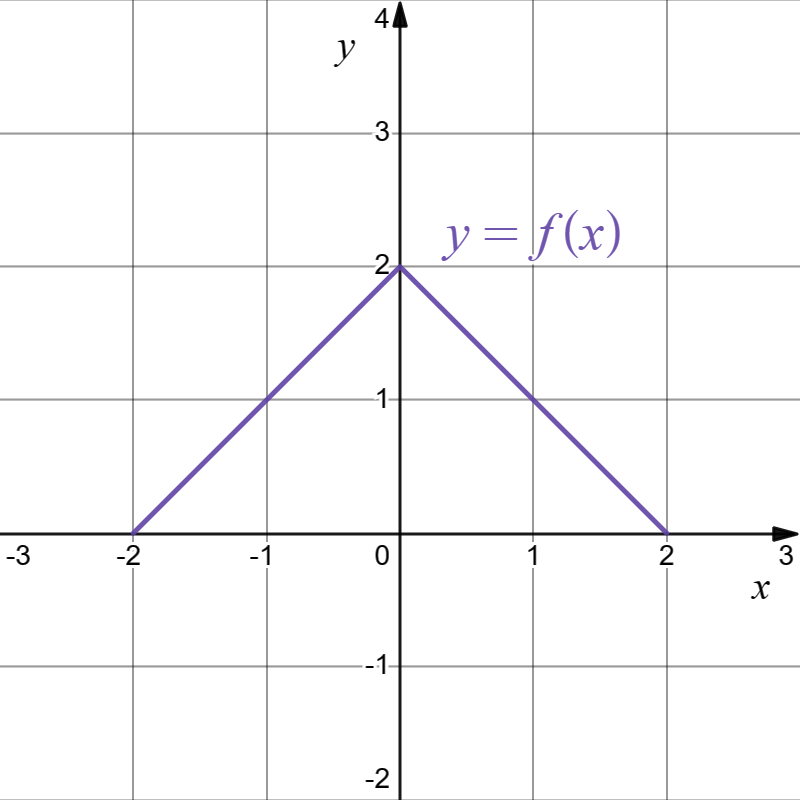
\includegraphics[width=0.5\textwidth]{figs/-abs(x)+2.png}
\end{example}

\newpage
\begin{example}
Sketch the graph of the function $g(x)=2\sqrt{3x-1}-4$ by a sequence of transformation applied on the graph of $f(x)=\sqrt{x}$.  
\end{example}

\begin{example}
  Find an equation of the function $y=g(x)$ whose graph is obtained from $f(x)=\sqrt{x}$ by the following transformations in the given order.
  \begin{enumerate}
    \item stretch vertically by a factor of 2
    \item shift downward 2 units
    \item shift 3 units to the left
    \item stretch horizontally by a factor $\dfrac{1}{2}$.
  \end{enumerate}
\end{example}

\newpage

\section*{Exercises}

\begin{exercise}
    Consider the functions $f(x)=x^2$, $g(x)=(x+1)^2-2$ and $h(x)=(x-2)^2+1$.
    \begin{enumerate}
      \item Describe how to get the graph of $g$ from the graph of $f$.
      \item Describe how to get the graph of $h$ from the graph of $g$.
    \end{enumerate}
\end{exercise}

\begin{exercise}
    Determine if the function is even, odd, or neither.\\
    \begin{enumerate*}
      \item $f(x)=1-x^2$.
      \item $g(x)=\sqrt[3]{-x}$.
      \item $g(x)=x^4-x^3$.
      \hfill\mbox{}
    \end{enumerate*}  
\end{exercise}

\newpage

\begin{exercise}
  Sketch the graph of the function $g(x)=2|3x-6| + 4$ by a sequence of transformation applied on the graph of $f(x)=|x|$.  
\end{exercise}

\begin{exercise}
  Find an equation of the function $y=g(x)$ whose graph is obtained from $f(x)=\sqrt[3]{x}$ by the following transformations in the given order.
  \begin{enumerate}
    \item Compress vertically by a factor of $\dfrac{1}{2}$.
    \item Reflect vertically.
    \item shift downward 2 units.
    \item Compress horizontal by a factor $2$.
    \item Shift 3 units to the right.
  \end{enumerate}
\end{exercise}

\newpage

\section{Inverse Functions}

\begin{definition}
  Let $y=f(x)$ be a one-to-one function with the domain $A$. A function \(f^{-1}(x)\) is an \textbf{inverse function} of \(f\) if \(f^{-1}(f(x))=x\) for all \(x\) in $A$.

The notation \(f^{-1}\) is read “\(f\) inverse.” 
\end{definition}
\begin{remark}
  \begin{enumerate}[series=PropertiesInverse]
    \item If $f$ is a one-to-one function, then it has a unique inverse function $f^{-1}$. Here is the proof. Suppose $g$ is also an inverse $f$. Then $f(g(x))=x=f(f^{-1}(x))$. Then $g(x)=f^{-1}(f(g(x)))=f^{-1}(f(f^{-1}(x)))=f^{-1}(x)$.
    \item Note that if $f^{-1}$ is the inverse of $f$, then $f$ is also the inverse of $f^{-1}$ that is $f(f^{-1})(x)=x$ for all $x$ in the domain of $f^{-1}$.
  \end{enumerate}
  \begin{multicols}{2}
    \begin{enumerate}[resume=PropertiesInverse]
      \item In general, $f^{-1}(x)\neq f(x)^{-1}$.
      \item The graphs of a one-to-one function $f$ and its inverse $f^{-1}$ are symmetric about the diagonal line $y=x$.\\
      \item Suppose $f$ has the domain $A$ and the range $B$, then $f^{-1}$ has the domain $B$ and the range $B$ (and vice verse).
      \vfill\null
    \end{enumerate}
    \columnbreak
\begin{center}
  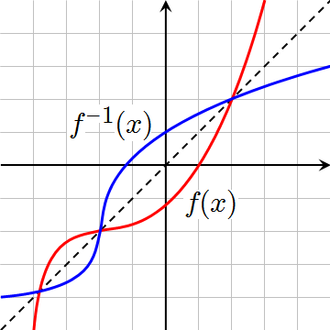
\includegraphics[width=0.25\textwidth]{figs/Inverse_Function_Graph.png}\\
 {\footnotesize The above graph of $f$ and $f^{-1}$ is taken from \href{https://en.wikipedia.org/wiki/Inverse_function}{Wikipedia}.}
\end{center}
\end{multicols}
\end{remark}

\begin{example}
  Let $f$ be a one-to-one function with \(f(3)=4\) and \(f(4)=5\). Find $f^{-1}(4)$.
\end{example}

\begin{example}
  Let $f(x)=\dfrac{1}{x-1}$ and $g(x)=\dfrac{x+1}{x}$. Determine if $g$ is the inverse function of $f$.
\end{example}


\newpage

\begin{example}
  Consider the function $f(x)=x^2+1$ with $x>0$. Sketch the graph of $y=f^{-1}(x)$ without finding its equation.
\end{example}

\begin{howto}
  Given a function $y=f(x)$, the inverse function is the solution $y$ of the equation $f(y)=x$. The domain and the range of $f$ and $f^{-1}$ can be obtained from the domains of $f$ and $f^{-1}$.
\end{howto}


\begin{example}
  Consider the function $f(x)=2x-3$. Find the inverse function $f^{-1}$ and its domain and range.
\end{example}

\begin{example}
  Consider the function $f(x)=\dfrac{x}{x-1}$. Find the inverse function $f^{-1}$ and its domain and range.
\end{example}

\newpage

\begin{example}
  Consider the function $f(x)=2(x+1)^3-1$. Find the inverse function $f^{-1}$ and its domain and range.
\end{example}

\begin{example}
  Consider the function $f(x)=\sqrt{x-2}$. Find the inverse function $f^{-1}$ and its domain and range.
\end{example}

\begin{example} Find the inverse of each of the following functions if it exists.
  \begin{center}
    \begin{tabular}{*{5}{l}}
      \hline
    Constant & Identity & Quadratic & Cubic & Reciprocal\\
    $f(x)=c$ & $f(x)=x$ & $f(x)=x^2$ & $f(x)=x^3$ & $f(x)=\dfrac{1}{x}$\\
    \hline
    Reciprocal squared & Cube Root & Square Root & Absolute Value & \\
    $f(x)=\dfrac{1}{x^2}$ & $f(x)=\sqrt[3]{x}$ & $f(x)=\sqrt{x}$ & $f(x)=|x|$ & \\ 
      \hline
    \end{tabular}
  \end{center}
\end{example}

\newpage

\section*{Exercises}

\begin{exercise}
  Let $f$ be a one-to-one function with \(f(-2)=-3\) and \(f(-3)=4\). Find $f^{-1}(-3)$.
\end{exercise}

\begin{exercise}
  Let \(f(x)=x^3-1\) and \(g(x)=\sqrt[3]{x+1}\). Is \(g=f^{-1}\)?
\end{exercise}

\begin{exercise}
  Consider the function $f(x)=\dfrac{1}{x-1}+1$. Sketch the graph of $f^{-1}$ without finding its equation.
\end{exercise}

\newpage

\begin{exercise}
  Consider the function $f(x)=\dfrac{1-x}{x+1}$. Find the inverse function $f^{-1}$ and its domain and range.
\end{exercise}

\begin{exercise}
  Consider the function $f(x)=3(x-1)^3+2$. Find the inverse function $f^{-1}$ and its domain and range.
\end{exercise}

\begin{exercise}
  Consider the function $f(x)=\sqrt{x+1}-1$. Find the inverse function $f^{-1}$ and its domain and range.
\end{exercise}


\newlecture
% !TeX root =  main.tex

\chapter{Polynomial and Rational Functions}

\section{Quadratic Functions}
\begin{definition}
  A function $f(x)=ax^2+bx+c$ with $a\ne 0$ is called a \textbf{quadratic function}. Its graph is called a \textbf{parabola}. By completing the square (let $h=-\dfrac{b}{2a}$ and $k=f(h)$), a quadratic function can be written in the \textbf{standard form} (or \textbf{vertex form}): $f(x)=a(x-h)^2+k$. The vertical line $x=-\dfrac{b}{2a}$ (or $x=h$) is called the \textbf{axis of symmetry}. The \textbf{vertex} $(h,k)$ is the intersection of the axis of symmetry and the parabola.
\end{definition}
\begin{note}
  The $y$-intercept of a quadratic function is $(0, f(0))$. The $x$-coordinates of $x$-intercepts are the zeros (or roots) of the function $f$, that is, the solutions of the equation $f(x)=0$.
\end{note}

\begin{example}
  Find the vertex form of the quadratic function $f(x)=2 x^{2} + 4 x + 1$ and determine the vertex, axis of symmetry, $x$-intercepts, and $y$-intercept of the function.
\end{example}

\begin{note}
  \begin{itemize}
    \item A quadratic function $f(x)=ax^2+bx+c$ can be obtained from $y=x^2$ by a combination of vertical stretch by a factor $|a|$, a vertical reflection if $a<0$, a vertical shift of $f\left(-\frac{b}{2a}\right)$ units, and a horizontal shift of $-\frac{b}{2a}$ units.
    \item The domain of a quadratic function is $(-\infty, \infty)$.
    \item If $a>0$, then the parabola opens upward, the function has an absolute minimum $f\left(-\frac{b}{2a}\right)$, and the domain of the function is $[f\left(-\frac{b}{2a}\right), \infty)$.
    \item If $a<0$, then the parabola opens downward, the function has an absolute maximum $f\left(-\frac{b}{2a}\right)$, and the domain of the function is $(-\infty,f\left(-\frac{b}{2a}\right)]$.
  \end{itemize}
\end{note}
\newpage

\begin{example}
 Find the vertex form equation for the quadratic function $g$ in figure below as a transformation of $f(x)=x^2$, and then simplify the equation into general form.

 \begin{tikzpicture}
  \begin{axis}[
  axis lines=middle,
  unit vector ratio=1 1,
  ymajorgrids=true,
  xmajorgrids=true,
  xmin=-3,
  xmax=5,
  ymin=-3,
  ymax=5,
  xtick={-10,-9,...,10},
  ytick={-6,-5,...,6},]
  \addplot[blue, line width=1.5pt, domain=-3:5] {1/2*(x-1)^2-2} node[pos=0.8, above left] {$y=g(x)$};
  \end{axis}
  \end{tikzpicture}
\end{example}
\vspace*{-0.2\textheight}

\begin{example}
  Find the domain and range of each function.\\
  \begin{enumerate*}
    \item $f(x)=3x^2+6x-5$.
    \item $f(x)=-2x^2+4-1$.\hfill\null
  \end{enumerate*}
\end{example}

\begin{example}
  A backyard farmer wants to enclose a rectangular space for a new garden within her fenced backyard. She has purchased 80 feet of wire fencing to enclose three sides, and she will use a section of the backyard fence as the fourth side.
\end{example}

\newpage

\begin{example}
  A local newspaper currently has 84,000 subscribers at a quarterly charge of \$30. Market research has suggested that if the owners raise the price to \$32, they would lose 5,000 subscribers. Assuming that subscriptions are linearly related to the price, what price should the newspaper charge for a quarterly subscription to maximize their revenue?
\end{example}

\begin{example}
  A ball is thrown upward from the top of a 40-foot-high building at a speed of 80 feet per second. The ball's height above ground can be modeled by the equation \(H(t)=-16t^2+80t+40\).
\begin{enumerate}
  \item When does the ball reach the maximum height?
  \item What is the maximum height of the ball?  
  \item When does the ball hit the ground?
\end{enumerate}
\end{example}

\newpage

\section*{Exercise}

\begin{exercise}
  For each of the following functions,
  \begin{enumerate*}[label={(\alph*)}]
    \item $f(x)=x^2-4x+1$,
    \item $f(x)=-2x^2-4x+1$,\hfill\null
  \end{enumerate*}
  \begin{enumerate}
    \item write the function in vertex form,
    \item find the axis of symmetry,
    \item find the vertex,
    \item find the $y$-intercept,
    \item find the $x$-intercepts if they exist,
    \item find the domain and range,
    \item find the global maximum or minimum if it exists.
  \end{enumerate}
\end{exercise}

\begin{exercise}
  Find the vertex form equation for the quadratic function $f$ in figure below, and then simplify the equation into general form.
 
  \begin{tikzpicture}
   \begin{axis}[
    width=0.6\textwidth,
   axis lines=middle,
   unit vector ratio=1 1,
   ymajorgrids=true,
   xmajorgrids=true,
   xmin=-4,
   xmax=2,
   ymin=-2,
   ymax=4,
   xtick={-10,-9,...,10},
   ytick={-6,-5,...,6},]
   \addplot[blue, line width=1.5pt, smooth,samples=100] {2*(x+1)^2-1} node[pos=0.2, right] {$y=f(x)$};
   \end{axis}
   \end{tikzpicture}
 \end{exercise}

\newpage

\begin{exercise}
  Find the dimensions of the rectangular parking lots producing the greatest area given that \(500\) feet of fencing will be used to for three sides.
\end{exercise}

\begin{exercise}
  A rocket is launched in the air. Its height, in meters above sea level, as a function of time, in seconds, is given by \(h(t)=-4.9t^2+229t+234\). Find the maximum height the rocket attains.
\end{exercise}

\begin{exercise}
  A soccer stadium holds \(62,000\) spectators. With a ticket price of \(\$11\), the average attendance has been \(26,000\). When the price dropped to \(\$9\), the average attendance rose to \(31,000\). Assuming that attendance is linearly related to ticket price, what ticket price would maximize revenue?
\end{exercise}

\newpage

\section{Power and Polynomial Functions}

\begin{definition}
  A \textbf{power function} is a function that can be represented in the form
\[f(x)=kx^p,\]
where \(k\) and \(p\) are real numbers, and \(k\) is known as the \textbf{coefficient}.
\end{definition}

\begin{example}
  Determine if the function is a power function.\\
  \begin{enumerate*}
    \item $f(x)=-2x^3$
    \item $f(x)=\dfrac{1}{x^2}$
    \item $f(x)=\sqrt[3]{x}$
    \item $f(x)=2^x$
    \item $f(x)=2x^2\cdot 3x^5$
    \item $f(x)=\dfrac{x}{x+1}$
  \end{enumerate*}
\end{example}

\begin{definition}
  The \textbf{end behavior} of a function $f$ is the general direction that the function $f$ approaches as $x$ goes to $\infty$ or $-\infty$. 
  
  We use an arrow $\to$ to describe ``goes to'' or ``approaches to''. 
  The notation $x\to \infty$ or $x\to -\infty$ means ``$x$ goes to infinity'' or ``$x$ goes to negative infinity'' respectively.
  The notation $f(x)\to \infty$ or $f(x)\to -\infty$ means ``$f(x)$ goes to infinity'' or ``$f(x)$ goes to negative infinity'' respectively.

  If $f(x)\to b$ as $x\to \infty$ or $x\to -\infty$, then we say the line $y=b$ is a \textbf{horizontal asymptote}.
\end{definition}

\begin{howto}
  To determine the end behavior of a function $f$, take a large positive number $N$. 
  
  If $f(N)$ is a large positive number, then $f(x)\to \infty$ as $x\to \infty$. 
  
  If $-f(N)$ is a large positive number, then $f(x)\to -\infty$ as $x\to \infty$.
  
  If $f(-N)$ is a large positive number, then $f(x)\to\infty$ as $x\to -\infty$. 
  
  If $-f(-N)$ is a large positive number, then $f(x)\to-\infty$ as $x\to -\infty$.
\end{howto}

\begin{example}
  Determine the end behavior(s) of the function.\\
  \begin{enumerate*}
    \item $f(x)=-2x^3$
    \item $f(x)=\dfrac{1}{x^2}$
    \item $f(x)=\sqrt[3]{x}$\hfill\null
  \end{enumerate*}
\end{example}

\newpage

\begin{definition}
  Let $n$ be a non-negative integer. A \textbf{polynomial function} of \textbf{degree} $n$ is a function that can be written in the form 
  \[f(x)=a_nx^n + \cdots + a_2x^2 + a_1x + a_0.\]
\begin{itemize}
  \item Each \(a_i\) is called a \textbf{coefficient}. 
  \item Each product \(a_ix^i\) is called a \textbf{term} of a polynomial function.
  \item The term $a_nx^n$ is called the \textbf{leading term}. The number $a_n$ is called the \textbf{leading coefficient}.
  \item The number $a_0$ is called the \textbf{constant term}.
\end{itemize}
\end{definition}

\begin{note}
  The end behavior of a polynomial function $f(x)=a_nx^2+\cdots +a_0$ of degree $n$ is completely determined by the end behavior of the power function $g(x)=a_nx^n$.
  
  The domain of a polynomial function is $(-\infty, \infty)$. The range of an odd degree polynomial function is also $(-\infty, \infty)$. The range of an even degree polynomial function is either $[y_\text{min}, \infty)$ if $a_n>0$ or $(-\infty, y_\text{max}]$ if $a_n<0$, where $y_\text{min}$ (respectively, $y_\text{max}$) is the absolute minimum (respectively, maximum) of the function. 
\end{note}

\begin{example}
  Determine the end behavior of the function.\\
  \begin{enumerate*}
    \item $f(x)=2x^4-3x+1$
    \item $g(x)=-3x^3+2x^2-x$
    \item $h(x)=-4x^6-7x^5+10x^4+2$\hfill\null
  \end{enumerate*}
\end{example}

\begin{example}
  Identify the degree, the leading therm and the end behavior of the polynomial function.\\
  \begin{enumerate*}
    \item $f(x)=-3x^2(x-1)(x+4)$
    \item $f(x)=2x^3(1-x)(x+1)$\hfill\null
  \end{enumerate*}
\end{example}

\newpage

\begin{definition}
  If $f$ is a polynomial function, then a number $c$ is called a \textbf{zero} of $f$ if $f(c)=0$.
\end{definition}

\begin{proposition}
  Let $f$ be a polynomial and $c$ a real number. Then the following are equivalent:
  \begin{enumerate}
    \item $c$ is a zero of $f$.
    \item $x=c$ is a solution of the equation $f(x)=0$.
    \item $x-c$ is a factor of $f(x)$.
    \item $(c,0)$ is an $x$-intercept of the function of $y=f(x)$.
  \end{enumerate}
\end{proposition}

\begin{example}
  Find $x$-intercepts and the $y$-intercept of the polynomial function $f(x)=x^{3} + 3 x^{2} - x - 3$.
\end{example}

\begin{example}
  Find $x$-intercepts and the $y$-intercept of the polynomial function $f(x)=x^4+2x^2-3$.
\end{example}

\begin{definition}
  A \textbf{turning point} (also known as a local extremum) is a point at which the function values change from increasing to decreasing or decreasing to increasing.
\end{definition}

\begin{theorem}[Fundamental Theorem of Algebra\footnotemark]
  A degree $n$ polynomial function has at least one complex zero.
\end{theorem}

\footnotetext{A relatively elementary proof can be found at \href{https://tinyurl.com/tFToA}{https://tinyurl.com/tFToA}.}

\begin{proposition}
  A degree $n$ polynomial function may have at most $n$ real zeros and $n-1$ turning points.
\end{proposition}

\newpage

\begin{example}
  Consider the polynomial function  $f(x)=(x-2)(x+1)(x-4)$. Determine the zeros, the number of turning points, the $x$-intercepts, and the $y$-intercept.
\end{example}


\begin{example}
  What can we conclude about the leading term of the polynomial function $y=f(x)$ represented by the graph below.\\
  \begin{tikzpicture}
    \begin{axis}[
    xmin=-4,
    xmax=4,
    ymin=-4,
    ymax=4,
    xtick={-10,-9,...,10},
    ytick={-10,-9,...,10},]
    \addplot[line width=1.5pt, smooth, samples=100, domain=-3:4] {1/4*(x)^(4)-2/3*(x)^(3)-1/2*(x)^(2)+2*(x)-3/2} node[pos=0.9, left] {$y=f(x)$};
    \end{axis}
  \end{tikzpicture}
\end{example}
\vspace*{-0.4\textheight}


\newpage

\section*{Exercises}

\begin{exercise}
  Find the degree and leading coefficient, and determined the end behavior for the given polynomial.\\
  \begin{enumerate*}
    \item $f(x)=-2x^4$
    \item $f(x)=2x^5-x^3$
    \item $f(x)=-2x(1-x^2)$
    \item $f(x)=(x^2-1)(2x-1)(x+2)$
  \end{enumerate*}
\end{exercise}

\begin{exercise}
  Find $x$-intercepts (if they exist) and the $y$-intercept of the polynomial function.\\
  \begin{enumerate*}
  \item $f(x)=-2x^4+x^2+1$
  \item $f(x)=2x+x^3-3x^5$
  \item $f(x)=x^{3} + x^{2} - 4 x - 4$
\end{enumerate*}
\end{exercise}

\newpage
\section{Graphs of Polynomial Functions}

\begin{definition}
  We say a zero $c$ of a polynomial function $f$ has the \textbf{multiplicity} $k$ if $f(x)=(x-c)^kg(x)$ and $c$ is not a zero of $g$.
\end{definition}

\begin{example}
  Find the zeros of the polynomial function $f(x)=x^3(x-1)^2(x-2)$ and determine their multiplicities.
\end{example}

\begin{example}
  A polynomial function $P$ of degree 3 has two zeros $1$ and $2$ with multiplicity $2$ and $1$ respectively. The $y$-intercept is $(0, -4)$. Find an equation for $P$.
\end{example}


\begin{note}[Local Graph Near a Zero]
  Let $f$ be a polynomial with positive leading coefficient and $c$ is a zero of $f$ of the multiplicity $m$. The local shape of a polynomial function with positive leading coefficient near a zero  is of one of the following types.
  \begin{center}
    \begin{tikzpicture}
      \begin{axis}[
        title={$k=1$},
        width=0.4\textwidth,
        xmin=-1,
        xmax=1,
        ymin=-1,
        ymax=1,
        grid=none,
        xtick={0},
        extra x ticks={0},
        xticklabel={$c$},
        ylabel=\empty,
        ytick=\empty,
        y axis line style={draw=none},
      ]
      \addplot[line width=1.5pt,domain=-1:1] {-1/4*x*(x-2)*(x+2)};
      \end{axis}
    \end{tikzpicture}\hfil
    \begin{tikzpicture}
      \begin{axis}[
        title={$k>1$ and $k$ is even},
        width=0.4\textwidth,
        xmin=-1,
        xmax=1,
        ymin=-1,
        ymax=1,
        grid=none,
        xtick={0},
        extra x ticks={0},
        xticklabel={$c$},
        ylabel=\empty,
        ytick=\empty,
        y axis line style={draw=none},
      ]
      \addplot[line width=1.5pt,domain=-1:1] {-1/2*x^2*(x-2)};
      \end{axis}
    \end{tikzpicture}\hfil
    \begin{tikzpicture}
      \begin{axis}[
        title={$k>1$ and $k$ is odd},
        width=0.4\textwidth,
        xmin=-1,
        xmax=1,
        ymin=-1,
        ymax=1,
        grid=none,
        xtick={0},
        extra x ticks={0},
        xticklabel={$c$},
        ylabel=\empty,
        ytick=\empty,
        y axis line style={draw=none},
      ]
      \addplot[line width=1.5pt,domain=-1:1] {-1/2*x^3*(x-2)};
      \end{axis}
    \end{tikzpicture}
  \end{center}
\end{note}

\newpage

\begin{example}
  Use the graph of the function of degree 6 in the figure below to identify the zeros of the function and their possible multiplicities.\\
  \begin{tikzpicture}
    \begin{axis}[
      width=0.6\textwidth,
      title={A polynomial of degree 6.},
      xmin=-2,
      xmax=3,
      ymin=-2,
      ymax=3,
      xtick={-3,-2,...,3},
      ytick={-3,-2,...,3}
    ]
    \addplot[line width=1.5pt, domain=-2:3] {1/4*x*(x+1)^2*(x-2)^3};
    \end{axis}
  \end{tikzpicture}
\end{example}


\begin{example}
  Find a polynomial of the least degree whose graph is given below.\\
  \begin{tikzpicture}
    \begin{axis}[
      width=0.6\textwidth,
      % title={A polynomial of degree 6.},
      xmin=-3,
      xmax=2,
      ymin=-3,
      ymax=2,
      xtick={-6,-5,...,3},
      ytick={-6,-5,...,3}
    ]
    \addplot[line width=1.5pt, domain=-3:2] {-(x-1)*x^3*(x+2)^2};
    \end{axis}
  \end{tikzpicture}
\end{example}

\newpage

\begin{definition}
  A \textbf{continuous} function has no breaks in its graph. A \textbf{smooth} function is a continuous function whose graph that has no sharp corners.
\end{definition}
\begin{note}
  Polynomial functions are smooth functions.
\end{note}

\begin{theorem}[Intermediate Value Theorem\footnotemark]
  If $f$ is a continuous function and $f(a)f(b)<0$, then there exists at least one value $c$ between $a$ and $b$ such that $f(c)=0$. In particular, the theorem holds true for polynomial functions. 
\end{theorem}
\footnotetext{A proof of the theorem can be found in \href{https://tinyurl.com/ivtcont}{https://tinyurl.com/ivtcont}.}
  
\begin{corollary}
  Let $f$ be a polynomial function, $a$ and $b$ real zeros of $f$. If $f$ has no other zeros between $a$ and $b$, then either $f(x)>0$ for all $x$ between $a$ and $b$ or $f(x)<0$ for all $x$ between $a$ and $b$.
\end{corollary}

\begin{theorem}[Rolle's Theorem for Polynomial Functions]
  Let $f$ be a polynomial function, $a$ and $b$ two zeros. Then $f$ has at lease one local extremum (turning point) between $a$ and $b$.
\end{theorem}
  
\begin{example}
  Determine if the polynomial function $f(x)=5x^4-2x^3-20$ has a zero on the interval $[1, 2]$.
\end{example}

\begin{howto}[Guideline on Graphing a Polynomial Function]
\begin{enumerate}
  \item Plot the $y$-intercept.
  \item Determine the real zeros and their multiplicities, and sketch local graph near $x$-intercepts.
  \item Determine the end behavior and sketch the graph of the left and right tails.
  \item Using symmetry to plot additional points if possible.
  \item Use test points to determine whether the graph of the polynomial lies above or below the $x$-axis over the intervals between zeros, and estimate the locations of turning points.
  \item Connect points and local graphs smoothly.
\end{enumerate}
\end{howto}

\newpage

\begin{example}
  Sketch the graph of the polynomial function $f(x)=(x-4)(x-1)^2 (x+3)$.  
\end{example}
\newpage

\section*{Exercises}

\begin{exercise}
  Find the $t$-intercepts and the $P$-intercept of the polynomial function $P(t)=3t^4-15t^3+12t^2$.
\end{exercise}

\begin{exercise}
    A polynomial function $P$ of degree 3 has two zeros $1$ and $2$ with multiplicity $2$ and $1$ respectively. The $y$-intercept is $(0, -4)$. Find an equation for $P$.
\end{exercise}

\newpage

\begin{exercise}
  Find a polynomial of the least degree whose graph is given below.\\
  \begin{tikzpicture}
    \begin{axis}[
      width=0.6\textwidth,
      % title={A polynomial of degree 6.},
      xmin=-3,
      xmax=2,
      ymin=-1,
      ymax=4,
      xtick={-6,-5,...,6},
      ytick={-6,-5,...,6}
    ]
    \addplot[line width=1.5pt, domain=-2.5:1.2] {-(x-1)*x^2*(x+2)^3};
    \end{axis}
  \end{tikzpicture}
\end{exercise}
\vspace*{-0.2\textheight}

\begin{exercise}
  Sketch the graph of the polynomial function $f(x)=x^{4} - 2 x^{3} + x^{2}$.
\end{exercise}

\newpage
\section{Dividing of Polynomials}

\begin{theorem}[Division Algorithm]
  Let $p(x)$ and $d(x)$ be two polynomial. Suppose that \(d(x)\) is non-zero and the degree of \(d(x)\) is less than or equal to the degree of \(f(x)\). Then there exist unique polynomials \(q(x)\) and \(r(x)\) such that
  \[p(x)=d(x)q(x)+r(x)\]
and the degree of $r(x)$ is less than the degree of $d(x)$.
\end{theorem}
\begin{definition}
 In the above theorem, $p(x)$ is called the \textbf{dividend}, $d(x)$ is called the \textbf{divisor}, $q(x)$ is called the \textbf{quotient} and $r(x)$ is called the \textbf{remainder}.
 If $r(x)=0$, then we say that $d(x)$ \textbf{divides} $p(x)$.
 
 A divison algorithm\footnotemark~ is an algorithm which computes the quotient and the reminder. 

 Polynomial long division is a divison algorithm. Another shorthand division algorithm is the synthetic division. 
\end{definition}
\footnotetext{See wikipedia page on \href{https://en.wikipedia.org/wiki/Polynomial_long_division}{Polynomial long division} for various division algorithms.}

\begin{example}
  Divide \(6x^3+11x^2-31x+15\) by \(3x-2\).
\end{example}

\begin{example}
  Divide \(4x^4+3x^2-1x+5\) by \(2x^2-x+3\).
\end{example}

\newpage
\begin{definition}
  Synthetic division is a shortcut that can be used when the divisor is linear binomial in the form $x-c$. In synthetic division, only the coefficients are used in the division process.
\end{definition}

\begin{example}
  Use synthetic division to divide $4x^3+10x^2-6x-20$ by $x+2$.
\end{example}

\begin{example}
  Use synthetic division to divide $-9x^4+10x^3+7x^2-6$ by $x-1$.
\end{example}

\newpage
\section*{Exercises}

  \begin{exercise}
    Divide $3x^2 - 7 x - 3$ by $3x-1$.
  \end{exercise}

  \begin{exercise}
    Divide $16 x^3 - 12 x^2 + 20 x - 3$ by $4x+5$.
  \end{exercise}

  \begin{exercise}
  Use synthetic division to divide $5x^2-3x-36$ by $x-3$.
  \end{exercise}

  \begin{exercise}
  Divide $2 x^4 + 4 x^3 - 3 x^2 - 5 x - 2$ by $x+2$.
  \end{exercise}

\newpage
\section{Zeros of Polynomials}

\begin{theorem}[The Remainder Theorem]
If a polynomial $f(x)$ is divided by $x-c$, then the remainder is the value $f(c)$.
\end{theorem}
\begin{example}
  Use the Remainder Theorem to evaluate $f(x)=6x^4-x^3-15x^2+2x-7$ at $x=2$.
\end{example}

\begin{theorem}[The Rational Zero Theorem]
Let $f(x)=a_nx^n+a_{n-1}x^{n-1}+\cdots +a_1x+a_0$ be polynomial with integer coefficients. Then every rational zero of $f(x)$ is in the form $\frac{p}{q}$, where $p$ is a factor of the constant term $a_0$ and $q$ is a factor of the leading coefficient $a_n$.
\end{theorem}
\begin{example}
  List all possible rational zeros of $f(x)=2x^4-5x^3+x^2-4$.
\end{example}

\begin{example}
  Find the zeros of $f(x)=4x^3-3x-1$.
\end{example}

\newpage

\begin{theorem}[Linear Factorization Theorem]
  Let $f(x)$ be a polynomial with the degree $n>1$ and the leading coefficient $a_n$. Then
  \[f(x)=a_n(x-c_1)(x-c_2)\cdots(x-c_n),\]
  where $c_i$ are complex numbers.
\end{theorem}

\begin{theorem}[Complex Conjugation Theorem]
  Let $f(x)$ be a polynomial. If $x-(a+b~i)$ is a factor of $f$, then $x-(a-b~i)$ is also a factor of $f$. 
\end{theorem}

\begin{example}
  Find a fourth degree polynomial with real coefficients that has zeros of $-3$, $2$, $i$, such that $f(-2)=100$.
\end{example}

\begin{theorem}[Descartes' Rule of Signs\footnotemark]
  Let $f(x)=a_nx^n+a_{n-1}x^{n-1}+\cdots+a_1x+a_0$ be a polynomial function with real coefficients.

  \begin{itemize}
    \item The number of positive real zeros counted with multiplicity is either equal to the number of sign changes of $f(x)$ or is less than the number of sign changes by an even integer.
    \item The number of negative real zeros counted with multiplicity is either equal to the number of sign changes of $f(-x)$ or is less than the number of sign changes by an even integer.
  \end{itemize}
\end{theorem}
\footnotetext{For a proof, see the blogpost \href{http://math1210blog.robertborgersen.info/2012/05/proof-of-descartes-rule-of-signs/}{Proof of Descartes' Rule of Signs}}

\begin{example}
  Use Descartes' Rule of Signs to determine the possible numbers of positive and negative real zeros for $f(x)=-x^4-3x^3+6x^2-4x-12$.
\end{example}

\newpage
\section*{Exercises}

\begin{exercise}
  Find all zeros of $f(x)=2x^3+5x^2-11x+4$.
\end{exercise}

\begin{exercise}
  Find all zeros of $f(x)=x^4 + 3 x^3 + 2 x^2 - 2 x - 4$.
\end{exercise}


\begin{exercise}
  Find a fourth degree polynomial with real coefficients that has zeros of $-1$, $2$, $1+i$, such that $f(-2)=10$.
\end{exercise}

\newpage

\section{Rational Functions}
\begin{definition}
  Let $p(x)$ and $q(x)$ be polynomials with $\deg(q(x))>0$. The function $f(x)=\dfrac{p(x)}{q(x)}$ is called a rational function. The domain of $f$ is $\{x\mid q(x)\ne 0\}$.
\end{definition}

\begin{example}
  Find the domain of $f(x)=\dfrac{x+3}{x^2-9}$.
\end{example}

\begin{definition}[Vertical Asymptote]
  A \textbf{vertical asymptote} of a function $f$ is a vertical line $x=a$ where the graph of $f$ goes to positive or negative infinity as $x$ approached $a$ from left or right, that is, as $x\rightarrow a^- ~\text{or}~ a^+$, $f(x)\rightarrow \infty$, or as $x\rightarrow a^- ~\text{or}~ a^+$, $f(x)\rightarrow -\infty$, where $x\to a^-$ ($a^+$) means $x$ approaches $a$ from the left (right).

  We say a function $f$ has a \textbf{removable discontinuities} (or \textbf{hole}) at $x=a$ if $f(x)\to b$ as $x\to a$ but $f(a)$ is undefined.
\end{definition}

\begin{proposition}
  Let $f=\dfrac{p(x)}{q(x)}$ be a rational function. If $p(a)=q(a)=0$, then $f$ has a hole at $a$. If $q(a)=0$ but $p(a)\ne 0$, then $f$ has a vertical asymptote $x=a$.
\end{proposition}

\begin{definition}[Horizontal Asymptote]
A \textbf{horizontal asymptote} of a function $f$ is a horizontal line $y=b$ where the graph of $f$ approaches to $b$ as $x$ goes to positive or negative infinity, that is,   
as $x\rightarrow \infty$, or $x\rightarrow -\infty$, $f(x)\rightarrow b$.
\end{definition}

\begin{definition}[Slanted Asysmptote]
  A \textbf{slanted asymptote} of a function $f$ is a line $y=mx+b$ with $m\ne 0$ where the graph of $f$ approaches to $mx+b$ as $x$ goes to positive or negative infinity, that is,   
as $x\rightarrow \infty$ or $x\rightarrow -\infty$, $f(x)\rightarrow mx+b$.
\end{definition}

\begin{note}
  For a rational function $f$, as $x\rightarrow \infty$ or $-\infty$, $f(x)$ approaches the asymptote only from one side of the line. This information will be helpful when sketching a graph.
\end{note}


\begin{proposition}
Let $f(x)=\dfrac{p(x)}{q(x)}=\dfrac{a_mx^m+a_{m-1}x^{m-1}+...+a_1x+a_0}{b_nx^n+b_{n-1}x^{n-1}+...+b_1x+b_0}$ be a rational function.
\begin{itemize}
  \item if $m<n$, then $f$ has a horizontal asymptote $x=0$;
  \item if $m=n$, then $f$ has a horizontal asymptote $x=\frac{a_m}{b_n}$;
  \item if $m=n+1$, then $f$ has a slated asysmptote $y=mx+b$, where $mx+b$ is the quotient of $\frac{p(x)}{q(x)}$.
  \item if $m>n+1$, then $f$ has no horizontal or slated asymptote;
\end{itemize}
\end{proposition}

\newpage

\begin{example}
  Use arrow notation to describe asymptotes of the function $f$ graphed in the figure.\\
  \begin{tikzpicture}
    \begin{axis}[
    xmin=-2,
    xmax=4,
    ymin=-1,
    ymax=5,
    xtick={-5,-4,...,6},
    ytick={-1,0,...,5},
    grid=none]
    \addplot[line width=1.5pt, restrict y to domain=-5:10, blue] {1/(x-1)+2} node[pos=0.8, above right] {$f$};
    \addplot+[dashed,mark=none] coordinates{(1,-1)(1,5)};
    \addplot[dashed, domain=-2:4] {2};
    \end{axis}
    \end{tikzpicture}
\end{example}
\vspace*{-0.2\textheight}
\begin{example}
  Use arrow notation to describe the slanted asymptote of the function $f$ graphed in the figure.\\
  \begin{tikzpicture}
    \begin{axis}[
    xmin=-3,
    xmax=5,
    ymin=-4,
    ymax=4,
    xtick={-5,-4,...,6},
    ytick={-4,-3,...,5},
    grid=none]
    \addplot[line width=1.5pt, restrict y to domain=-5:5, blue] {1/(x-1)+x-1} node[pos=0.7, above] {$f$};
    \addplot+[dashed,mark=none] coordinates{(1,-4)(1,4)};
    \addplot[dashed,domain=-4:4] {x-1};
    \end{axis}
    \end{tikzpicture}
\end{example}
\vspace*{-0.2\textheight}

\begin{example}
Find the asymptotes of the rational function $f(x)=\dfrac{x^2+1}{2x^2-3x+1}$ if they exist.
\end{example}

\newpage

\begin{example}
Find the asymptotes of the rational function $f(x)=\dfrac{- x^{2} + 3 x - 1}{x - 1}$ if they exist.
\end{example}

\begin{example}
  Find the asymptotes and holes of the function
$f(x)=\dfrac{x^{2} + x - 6}{x^{3} - 2 x^{2} - x + 2}$ if they exist.
\end{example}

\newpage

\begin{howto}[Sketch a Graph of a Rational Function]
  \begin{enumerate}
  \item Find the $y$-intercept and plot it.
  \item Find the $x$-intercept(s) and plot them.
  \item Find all vertical asymptotes and graph them as dashed lines.
  \item Find the horizontal asymptote or the slant asymptote (or neither), and graph the asymptote as a dashed line.
  \item Plot a test point in each interval whose boundary values are zeros of the denominator.
  \item Sketch the function based on the information found above.
  \end{enumerate}
\end{howto}

\begin{example}
  Sketch a graph of  $f(x)=\dfrac{(x+2)(x-3)}{(x+1)^2(x-2)}$.
\end{example}

\newpage

\section*{Exercises}

\begin{example}
  Find asymptotes of the rational function $f(x)=\dfrac{3x^2-1}{x^2+4x-5}$
\end{example}

\begin{exercise}
  Find asymptotes of the rational function $f(x)=\dfrac{x^{2}}{x + 1}$.
\end{exercise}

\begin{exercise}
  Find asymptotes and holes of the rational function $f(x)=\dfrac{(x-1)(x-2)}{x^2-4}$.
\end{exercise}
\newpage

\begin{exercise}
  Sketch a graph of the rational function $f(x)=\dfrac{(x+2)^2(x-1)}{(x+1)^2(x-2)}$.
\end{exercise}

\begin{exercise}
  Sketch a graph of the rational function  $f(x)=\dfrac{4(x+2)(x-3)^3}{(x+1)(x-2)^2}$.
\end{exercise}

\newpage
\section{Polynomial and Rational Inequalities}
\begin{howto}[Solve Polynomial or Rational Inequalities]
\begin{enumerate}
  \item Rewrite the inequality into the form $f(x)\text{~inequality symbol~} 0$.
  \item Find real zeros of $f$ and its denominator.
  \item Break then number line into intervals using zeros from the previous step.
  \item Choose a test point from each interval to determine the sign of $f$.
  \item Determine the solutions (intervals in which the test point satisfies the inequality) and whether the boundary values of the intervals should be included.
\end{enumerate}
\end{howto}

\begin{example}
  Solve the inequality $x^{2} \le 7 x - 6$.
\end{example}

\begin{example}
  Solve the inequality $2 x^{3} - 3 x^{2} >  3 x - 2$.
\end{example}

\newpage

\begin{example}
  Solve the inequality $\dfrac{4-x}{x - 1}< 2$.
\end{example}

\begin{example}
  Solve the inequality $\dfrac{6 x}{(x + 1) (x + 2)}\ge 1$.
\end{example}


\newpage
\section*{Exercises}

\begin{exercise}
  Solve the inequality $-x^2>5x-6$.
\end{exercise}

\begin{exercise}
  Solve the inequality $2 x^{3} + x^{2} \le 2 x + 1$.
\end{exercise}

\newpage

\begin{exercise}
  Solve the inequality $1\ge \dfrac{x-1}{2x+1}$.
\end{exercise}

\begin{exercise}
  Solve the inequality $\dfrac{x+8}{x^2-4}<1$.
\end{exercise}


\newlecture
% !TeX root =  main.tex

\section{Functions}


\begin{definition}[Function]

    A parabola is the set of all points in the plane that are equidistant from a fixed point $F$ (called the \textbf{focus}) and a fixed line $l$ (called the \textbf{directrix}).
\end{definition}
\begin{wrapfigure}[10]{r}{0.4\textwidth}
    \centering
    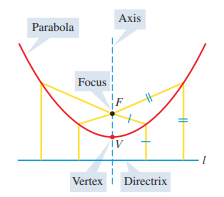
\includegraphics[width=0.3\textwidth,keepaspectratio]{figs/parabola-concepts.png}
\end{wrapfigure}
The \textbf{axis of symmetry} is the line that runs through the focus perpendicular to the directrix. The \textbf{vertex} $V$ is the intersection of the parabola and the axis of symmetry. Equivalently, the vertex lies halfway between the focus and the directrix.

\begin{theorem}[Parabola with vertical axis]
    A parabola has an equation $x^2=4py$ if and only if two of the following properties are satisfied:
    \begin{enumerate}[sepno]
        \item the vertex is $V(0, 0)$;
        \item the focus is $F(0, p)$;
        \item the directrix is $y=-p$.
    \end{enumerate}

    The parabola opens upward if $p>0$ or downward if $p<0$.
\end{theorem}

\begin{theorem}[Parabola with horizontal axis]
    A parabola has an equation $y^2=4px$ if and only if two of the following properties are satisfied:
    \begin{enumerate}[sepno]
        \item the vertex is $V(0, 0)$;
        \item the focus is $F(p, 0)$;
        \item the directrix is $x=-p$.
    \end{enumerate}

    The parabola opens to the right if $p>0$ or to the left if $p<0$.
\end{theorem}
\begin{center}
    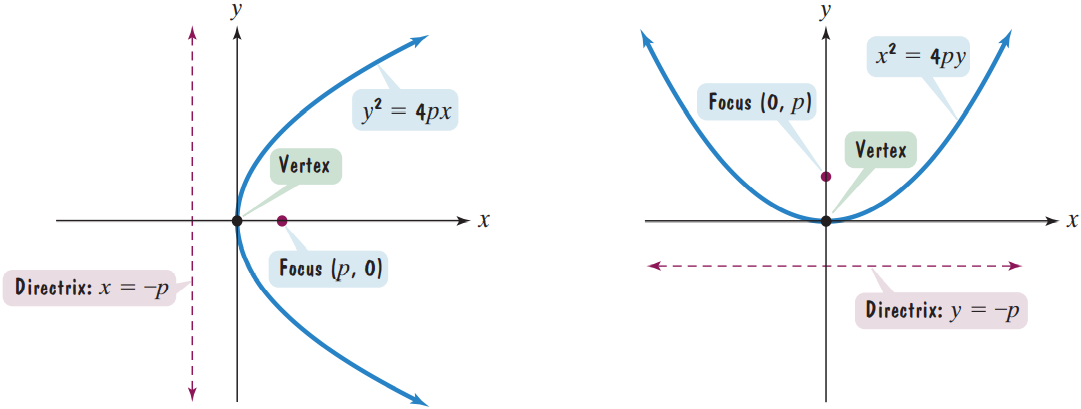
\includegraphics[width=0.8\textwidth,keepaspectratio]{figs/ParabolaGraphs.png}
\end{center}
The equations in the above theorems are called the standard form of the equation of a parabola with its vertex at the origin.

\begin{example}
    Find an equation of the parabola with the vertex $V(0,0)$ and focus $F(0,2)$.
\end{example}
\begin{solution}
    Because the vertex is $V(0, 0)$ and the focus is $F(0, 2)$. We know that $p=2$ and the axis of symmetry is vertical. Therefore, the parabola is defined by $x^2=8y$ by the theorem.
\end{solution}

\begin{example}
    Find the focus and directrix of the parabola $y=-x^2$.
\end{example}
\begin{solution}
    The equation of the parabola can be written as $x^2=-y$. Comparing with the standard form equation $x^2=4py$, we see that $4p=-1$ which implies $p=-\frac14$. So the focus is $\left(0, -\frac14\right)$ and the directrix is $y=-\left(-\frac14\right)$ which simplifies into $y=\frac{1}{4}$.
\end{solution}

The line segment that runs through the focus perpendicular to the
axis, with endpoints on the parabola, is called the \textbf{latus rectum}, and its length is the \textbf{focal diameter} of the parabola.

Because the latus rectum is parallel to the directrix and points on a parabola are equidistant from the focus and the directrix. The focal diameter equals the distance from the focus to the directrix. In particular, for a parabola with the vertex at the origin and the focus on a coordinate axis, the focal diameter is $|4p|$.

\begin{example}
    Find the focus, directrix, and focal diameter of the parabola $y=\frac{1}{2}x^2$.
\end{example}
\begin{solution}
    Rewriting the equation into standard form yields $x^2=2y$. Then $4p=2$ and $p=\frac{1}{2}$. Since the axis of symmetry is vertical, the focus is $(0, \frac12)$, the directrix is $y=-\frac12$, and the focal diameter is $|4p|=4\cdot\frac12=2$.
\end{solution}

\begin{example}
    A searchlight has a parabolic reflector that forms a “bowl,” which is 12 in. wide from rim to rim and 8 in. deep.  If the filament of the light bulb is located at the focus, how far from the vertex of the reflector is it?
\end{example}
\vspace{-2\baselineskip}
\begin{center}
    \noindent
    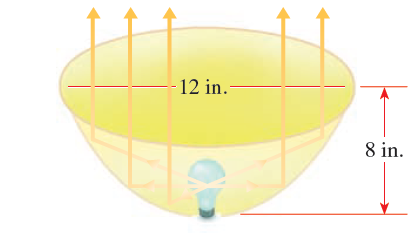
\includegraphics[height=8\baselineskip,keepaspectratio]{figs/SearchlightReflector1.png}
    \hspace{2em}
    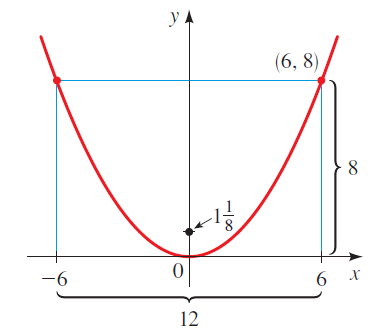
\includegraphics[height=9\baselineskip,keepaspectratio]{figs/SearchlightReflector2.png}
\end{center}

\begin{solution}
    We may assume the vertex is at the origin and the light bulb is at $F(0, p)$.
    Since the reflector is parabolic, that is the vertical section through the vertex and the light bulb is a parabola, an equation of the parabola is $x^2=4py$.
    Because the parabola is symmetric with respect to the axis of symmetry which is the vertical line passing through the vertex and the focus, there is a point $(6,8)$ on the parabola. It then follows that
    \[6^2=4p\cdot 8.\]
    Solving for $p$ yields $p=\frac{9}{8}$. So the light bulb is $\frac{9}{8}$ in. above the vertex of the reflector.
\end{solution}

\section{Ellipses}

\begin{definition}[Geometric Definition of an Ellipse]
    An \textbf{ellipse} is the set of all points in the plane the sum of whose distances from two fixed points $F_1$ and $F_2$ is a constant. These two fixed points are the \textbf{foci} (plural of focus) of the ellipse.
\end{definition}

\begin{definition}
    The midpoint of the line segment joining the foci is called the \textbf{center} of the ellipse.

    The line segment through the foci with endpoints on the ellipse is called the \textbf{major axis}

    The line segment perpendicular to the major axis through the center with endpoints on the ellipse is the \textbf{minor axis}.

    The intersections of the ellipse and the major axis are called the \textbf{vertices} of the ellipse.

    The distance of the foci to the center is called the \textbf{focal distance} or \textbf{linear eccentricity}.

\end{definition}

\begin{proposition}
    Suppose the length of the major axis is $2a$, the length of the minor axis is $2b$, and the linear eccentricity is $c$. Then
    \[a^2=b^2+c^2.\]
\end{proposition}

\begin{theorem}[Ellipse centered at the origin and with the major axis along the $x$-axis]
An ellipse has an equation $\frac{x^2}{a^2}+\frac{y^2}{b^2}=1$ if and only if the foci are $(\pm \sqrt{a^2-b^2}, 0)$ and the vertices are $(\pm a, 0)$, where $a>0$.
\end{theorem}

\begin{theorem}[Ellipse centered at the origin and with the major axis along the $y$-axis]
An ellipse has an equation $\frac{x^2}{b^2}+\frac{y^2}{a^2}=1$ if and only if the foci are $(0, \pm \sqrt{a^2-b^2})$ and the vertices are $(0, \pm a)$, where $a>0$.
\end{theorem}

\begin{center}
    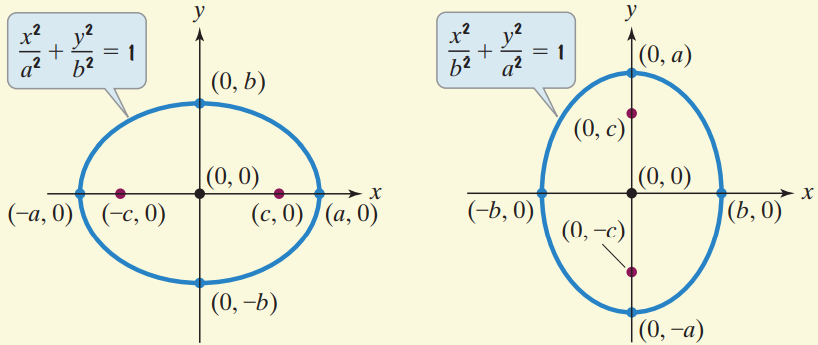
\includegraphics[width=0.8\textwidth,keepaspectratio]{figs/EllipseGraphs.png}
\end{center}

The questions of ellipses in the above theorems are called the \textbf{standard form}.

\begin{example}
    An ellipse has the equation $\dfrac{x^2}{9}+\dfrac{y^2}{4}=1$.
    Find the foci, the vertices, and the lengths of the major and minor axes. Sketch the graph.
\end{example}
\vspace*{6\baselineskip}

\begin{example}
    Find the foci of the ellipse $16x^2+9y^2=144$.
\end{example}
\vspace*{6\baselineskip}

\begin{example}
    Find an equation of the ellipse with the vertices $(\pm 4, 0)$ and the foci $(\pm 2, 0)$.
\end{example}
\vspace*{6\baselineskip}

\begin{definition}
    The eccentricity $e$ of an ellipse is defined as
    \[e=\dfrac{\text{focal distance}}{\frac12\left(\text{length of the major axis}\right)}.\]
    \begin{center}
        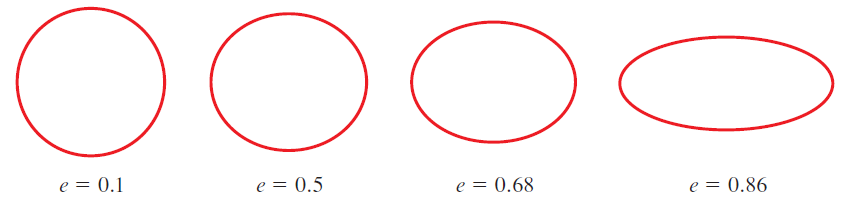
\includegraphics[scale=0.8]{figs/EllipseWithVariousEccentricities.png}
    \end{center}
\end{definition}

For an ellipse centered at the origin and with the major axis along a coordinate axis, the eccentricity is $e=\dfrac ca$.

\begin{example}
    Find the equation of the ellipse with foci $(0, \pm8)$ and the eccentricity $e=\frac45$.
\end{example}
\vspace*{8\baselineskip}

\section{Hyperbola}

\begin{definition}[Geometric Definition of a Hyperbola]
    A \textbf{hyperbola} is the set of all points in the plane, the difference of whose distances
    from two fixed points $F_1$ and $F_2$ is a constant. These two
    fixed points are the \textbf{foci} of the hyperbola.
\end{definition}

\begin{definition}
    The line segment containing the foci with endpoints on the hyperbola is called the \textbf{transverse axis}.

    The endpoints of the transverse axis are called the \textbf{vertices} of the hyperbola.

    The midpoint of the line segment joining the foci is the \textbf{center} of the hyperbola.

    The distance of the foci to the center is called the \textbf{focal distance} or \textbf{linear eccentricity}.

    The hyperbola consists of two separate curves, called \textbf{branches}, that are symmetric with respect to the transverse axis, conjugate
    axis, and center. \end{definition}


\begin{theorem}[Hyperbola centered at the origin and with the transverse axis along the $x$-axis]
A hyperbola has an equation $\frac{x^2}{a^2}-\frac{y^2}{b^2}=1$ if and only if the foci are $(\pm \sqrt{a^2+b^2}, 0)$ and the vertices are $(\pm a, 0)$.
\end{theorem}

\begin{theorem}[Hyperbola centered at the origin and with the transverse axis along the $y$-axis]
A hyperbola has an equation $\frac{x^2}{b^2}-\frac{y^2}{a^2}=1$ if and only if the foci are $(0, \pm \sqrt{a^2+b^2})$ and the vertices are $(0, \pm a)$.
\end{theorem}

\begin{center}
    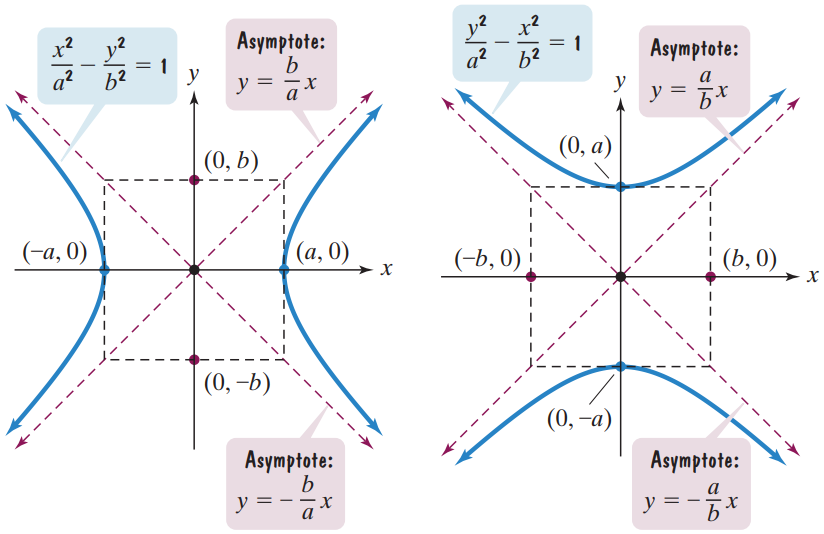
\includegraphics[width=0.8\textwidth,keepaspectratio]{figs/HyperbolaGraphs.png}
\end{center}

\begin{definition}
    A horizontal or oblique \textbf{asymptote} of a graph is a line with the property that the distance from the line to points on the graph approaches 0 as $x\to-\infty$ or as $x\to\infty$.
\end{definition}

A parabola has two asymptotes which are intersect at the center and symmetric with respect to the center or each axis.

\begin{proposition}[Characterization of hyperbola by asymptotes]
    A hyperbola has an equation $\dfrac{x^2}{a^2}-\dfrac{y^2}{b^2}=k$ if and only if its asymptotes are $y=\pm\dfrac{b}{a}x$ where $k$ is a non-zero real number.
\end{proposition}

The rectangle whose diagonals are along the aymptotes and with one side passing through a vertex of a hyperbola is called the \textbf{central box}.

The line segment through the center, perpendicular to the transverse axis with endpoints on the the central rectangle is the \textbf{conjugate axis}.

\begin{center}
    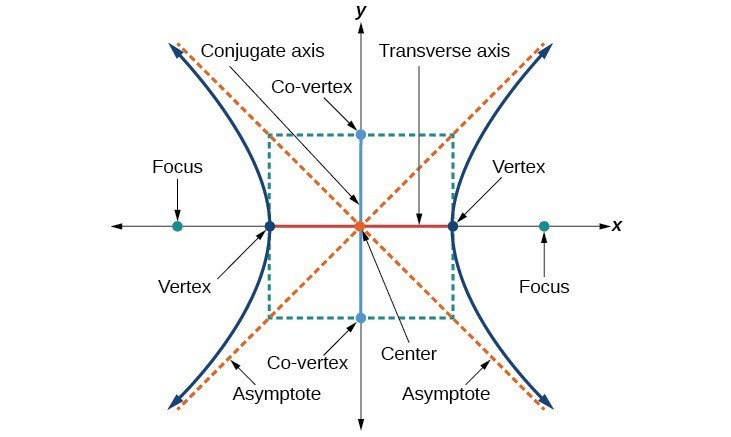
\includegraphics[width=0.7\textwidth,keepaspectratio]{figs/KeyConceptsOfHyperbola.jpg}
\end{center}

\begin{example}
    A hyperbola has the equation $9x^2-16y^2=121$.
    Find the vertices, foci, length of the transverse axis, and asymptotes. Sketch the graph.
\end{example}
\vspace*{8\baselineskip}

\begin{example}
    Find the vertices, foci, length of the transverse axis, and asymptotes of the hyperbola $x^2-9y^2+9=0$. Sketch the graph.
\end{example}
\vspace*{8\baselineskip}

\begin{example}
    Find the equation of the hyperbola with vertices $(\pm 3, 0)$ and foci $(\pm 4, 0)$.
\end{example}
\vspace*{8\baselineskip}

\begin{example}
    Find the equation and the foci of the hyperbola with vertices $(0,\pm 2)$ and asymptotes $y=\pm2x$.
\end{example}
\vspace*{8\baselineskip}

\section*{Practice}

\begin{exercise}
    Find the vertex, focus, and directrix of the parabola. Sketch the graph.\\
    \begin{enumerate*}
        \item $x^2=-8y$.
        \item $y^2=12x$.
        \item $x^2+6y=0$.
        \item $2x-y^2=0$.
    \end{enumerate*}
\end{exercise}
\vspace*{10\baselineskip}

\begin{exercise}
    An equation of an ellipse is given. Find the center, vertices, and foci of the ellipse, and the lengths of the major and minor axes. Sketch the graph.\\
    \begin{enumerate*}
        \item $\dfrac{x^2}{9}+\dfrac{y^2}{25}=1$.
        \item $\dfrac{y^2}{9}+\dfrac{x^2}{25}=1$.
        \item $9x^2+25y^2=1$.
        \item $25x^2+9y^2-16=0$.
    \end{enumerate*}
\end{exercise}
\vspace*{10\baselineskip}

\begin{exercise}
    An equation of an ellipse is given. Find the center, vertices, foci, and asymptotes of the hyperbola. Sketch the graph.\\
    \begin{enumerate*}
        \item $\dfrac{x^2}{9}-\dfrac{y^2}{25}=1$.
        \item $\dfrac{y^2}{9}-\dfrac{x^2}{25}=1$.
        \item $9x^2-25y^2=1$.
        \item $25x^2-9y^2-4=0$.
    \end{enumerate*}
\end{exercise}
\vspace*{10\baselineskip}

\begin{exercise}
    Find an equation for
    the conic section with the given properties.
    \begin{enumerate}
        \item The parabola with vertex at the origin and focus $(0, 5)$.
        \item The parabola with vertex at the origin and the directrix $x=-2$.
        \item The ellipse with vertices $(\pm 2, 0)$ and foci $(\pm 1, 0)$.
        \item the ellipse with foci $(0,\pm 3)$ and the eccentricity $e=\frac34$.
        \item The hyperbola with foci $(0,\pm 3)$ and vertices $(\pm 2, 0)$.
        \item The hyperbola with foci $(\pm 5, 0)$ and asymptotes $y=\pm\frac34$.
    \end{enumerate}
\end{exercise}

\begin{exercise}
    Find an question for the conic section with the given graph.
    \begin{enumerate}
        \item \mbox{}

        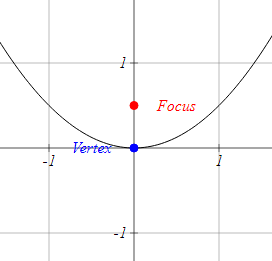
\includegraphics[width=0.3\textwidth]{figs/ParabolaEqFromGraph.png}
        \item \mbox{}

        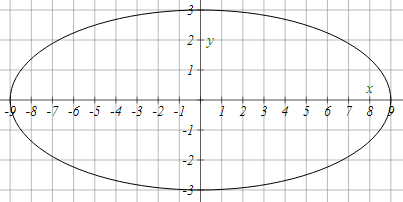
\includegraphics[width=0.4\textwidth]{figs/EllipseEqFromGraph.png}
        \item\mbox{}

        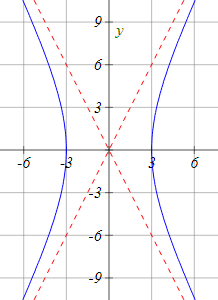
\includegraphics[width=0.3\textwidth]{figs/HyperbolaEqFromGraph.png}
    \end{enumerate}
\end{exercise}


\newlecture
% !TeX root =  main.tex

\section{Functions}


\begin{definition}[Function]

    A parabola is the set of all points in the plane that are equidistant from a fixed point $F$ (called the \textbf{focus}) and a fixed line $l$ (called the \textbf{directrix}).
\end{definition}
\begin{wrapfigure}[10]{r}{0.4\textwidth}
    \centering
    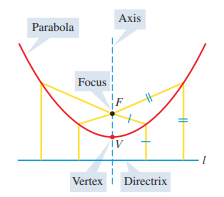
\includegraphics[width=0.3\textwidth,keepaspectratio]{figs/parabola-concepts.png}
\end{wrapfigure}
The \textbf{axis of symmetry} is the line that runs through the focus perpendicular to the directrix. The \textbf{vertex} $V$ is the intersection of the parabola and the axis of symmetry. Equivalently, the vertex lies halfway between the focus and the directrix.

\begin{theorem}[Parabola with vertical axis]
    A parabola has an equation $x^2=4py$ if and only if two of the following properties are satisfied:
    \begin{enumerate}[sepno]
        \item the vertex is $V(0, 0)$;
        \item the focus is $F(0, p)$;
        \item the directrix is $y=-p$.
    \end{enumerate}

    The parabola opens upward if $p>0$ or downward if $p<0$.
\end{theorem}

\begin{theorem}[Parabola with horizontal axis]
    A parabola has an equation $y^2=4px$ if and only if two of the following properties are satisfied:
    \begin{enumerate}[sepno]
        \item the vertex is $V(0, 0)$;
        \item the focus is $F(p, 0)$;
        \item the directrix is $x=-p$.
    \end{enumerate}

    The parabola opens to the right if $p>0$ or to the left if $p<0$.
\end{theorem}
\begin{center}
    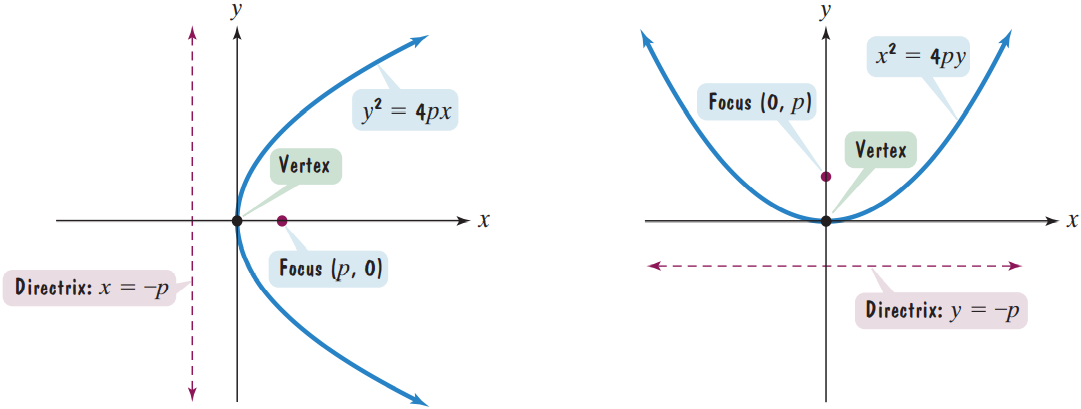
\includegraphics[width=0.8\textwidth,keepaspectratio]{figs/ParabolaGraphs.png}
\end{center}
The equations in the above theorems are called the standard form of the equation of a parabola with its vertex at the origin.

\begin{example}
    Find an equation of the parabola with the vertex $V(0,0)$ and focus $F(0,2)$.
\end{example}
\begin{solution}
    Because the vertex is $V(0, 0)$ and the focus is $F(0, 2)$. We know that $p=2$ and the axis of symmetry is vertical. Therefore, the parabola is defined by $x^2=8y$ by the theorem.
\end{solution}

\begin{example}
    Find the focus and directrix of the parabola $y=-x^2$.
\end{example}
\begin{solution}
    The equation of the parabola can be written as $x^2=-y$. Comparing with the standard form equation $x^2=4py$, we see that $4p=-1$ which implies $p=-\frac14$. So the focus is $\left(0, -\frac14\right)$ and the directrix is $y=-\left(-\frac14\right)$ which simplifies into $y=\frac{1}{4}$.
\end{solution}

The line segment that runs through the focus perpendicular to the
axis, with endpoints on the parabola, is called the \textbf{latus rectum}, and its length is the \textbf{focal diameter} of the parabola.

Because the latus rectum is parallel to the directrix and points on a parabola are equidistant from the focus and the directrix. The focal diameter equals the distance from the focus to the directrix. In particular, for a parabola with the vertex at the origin and the focus on a coordinate axis, the focal diameter is $|4p|$.

\begin{example}
    Find the focus, directrix, and focal diameter of the parabola $y=\frac{1}{2}x^2$.
\end{example}
\begin{solution}
    Rewriting the equation into standard form yields $x^2=2y$. Then $4p=2$ and $p=\frac{1}{2}$. Since the axis of symmetry is vertical, the focus is $(0, \frac12)$, the directrix is $y=-\frac12$, and the focal diameter is $|4p|=4\cdot\frac12=2$.
\end{solution}

\begin{example}
    A searchlight has a parabolic reflector that forms a “bowl,” which is 12 in. wide from rim to rim and 8 in. deep.  If the filament of the light bulb is located at the focus, how far from the vertex of the reflector is it?
\end{example}
\vspace{-2\baselineskip}
\begin{center}
    \noindent
    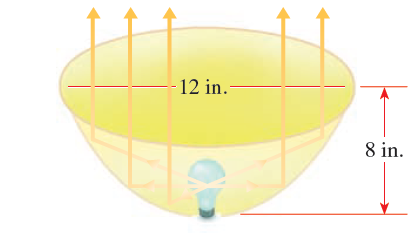
\includegraphics[height=8\baselineskip,keepaspectratio]{figs/SearchlightReflector1.png}
    \hspace{2em}
    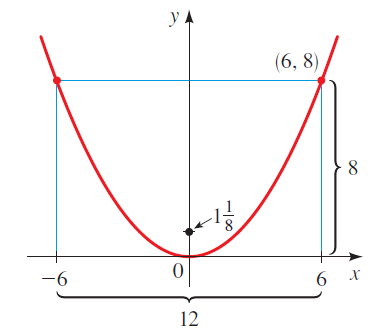
\includegraphics[height=9\baselineskip,keepaspectratio]{figs/SearchlightReflector2.png}
\end{center}

\begin{solution}
    We may assume the vertex is at the origin and the light bulb is at $F(0, p)$.
    Since the reflector is parabolic, that is the vertical section through the vertex and the light bulb is a parabola, an equation of the parabola is $x^2=4py$.
    Because the parabola is symmetric with respect to the axis of symmetry which is the vertical line passing through the vertex and the focus, there is a point $(6,8)$ on the parabola. It then follows that
    \[6^2=4p\cdot 8.\]
    Solving for $p$ yields $p=\frac{9}{8}$. So the light bulb is $\frac{9}{8}$ in. above the vertex of the reflector.
\end{solution}

\section{Ellipses}

\begin{definition}[Geometric Definition of an Ellipse]
    An \textbf{ellipse} is the set of all points in the plane the sum of whose distances from two fixed points $F_1$ and $F_2$ is a constant. These two fixed points are the \textbf{foci} (plural of focus) of the ellipse.
\end{definition}

\begin{definition}
    The midpoint of the line segment joining the foci is called the \textbf{center} of the ellipse.

    The line segment through the foci with endpoints on the ellipse is called the \textbf{major axis}

    The line segment perpendicular to the major axis through the center with endpoints on the ellipse is the \textbf{minor axis}.

    The intersections of the ellipse and the major axis are called the \textbf{vertices} of the ellipse.

    The distance of the foci to the center is called the \textbf{focal distance} or \textbf{linear eccentricity}.

\end{definition}

\begin{proposition}
    Suppose the length of the major axis is $2a$, the length of the minor axis is $2b$, and the linear eccentricity is $c$. Then
    \[a^2=b^2+c^2.\]
\end{proposition}

\begin{theorem}[Ellipse centered at the origin and with the major axis along the $x$-axis]
An ellipse has an equation $\frac{x^2}{a^2}+\frac{y^2}{b^2}=1$ if and only if the foci are $(\pm \sqrt{a^2-b^2}, 0)$ and the vertices are $(\pm a, 0)$, where $a>0$.
\end{theorem}

\begin{theorem}[Ellipse centered at the origin and with the major axis along the $y$-axis]
An ellipse has an equation $\frac{x^2}{b^2}+\frac{y^2}{a^2}=1$ if and only if the foci are $(0, \pm \sqrt{a^2-b^2})$ and the vertices are $(0, \pm a)$, where $a>0$.
\end{theorem}

\begin{center}
    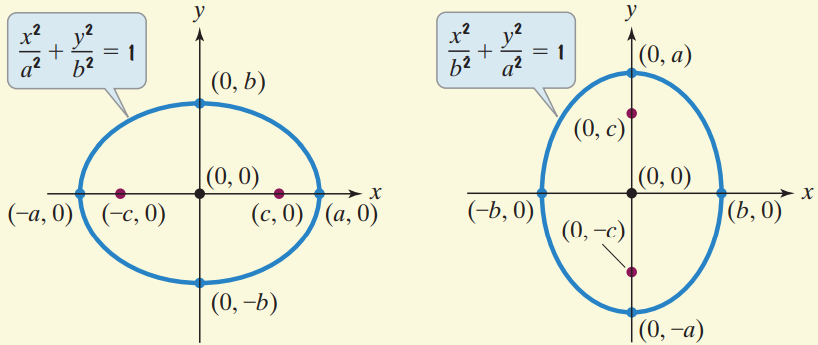
\includegraphics[width=0.8\textwidth,keepaspectratio]{figs/EllipseGraphs.png}
\end{center}

The questions of ellipses in the above theorems are called the \textbf{standard form}.

\begin{example}
    An ellipse has the equation $\dfrac{x^2}{9}+\dfrac{y^2}{4}=1$.
    Find the foci, the vertices, and the lengths of the major and minor axes. Sketch the graph.
\end{example}
\vspace*{6\baselineskip}

\begin{example}
    Find the foci of the ellipse $16x^2+9y^2=144$.
\end{example}
\vspace*{6\baselineskip}

\begin{example}
    Find an equation of the ellipse with the vertices $(\pm 4, 0)$ and the foci $(\pm 2, 0)$.
\end{example}
\vspace*{6\baselineskip}

\begin{definition}
    The eccentricity $e$ of an ellipse is defined as
    \[e=\dfrac{\text{focal distance}}{\frac12\left(\text{length of the major axis}\right)}.\]
    \begin{center}
        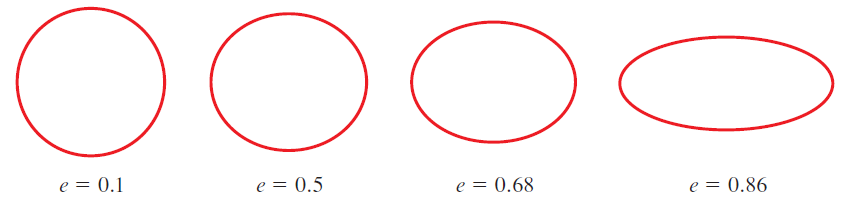
\includegraphics[scale=0.8]{figs/EllipseWithVariousEccentricities.png}
    \end{center}
\end{definition}

For an ellipse centered at the origin and with the major axis along a coordinate axis, the eccentricity is $e=\dfrac ca$.

\begin{example}
    Find the equation of the ellipse with foci $(0, \pm8)$ and the eccentricity $e=\frac45$.
\end{example}
\vspace*{8\baselineskip}

\section{Hyperbola}

\begin{definition}[Geometric Definition of a Hyperbola]
    A \textbf{hyperbola} is the set of all points in the plane, the difference of whose distances
    from two fixed points $F_1$ and $F_2$ is a constant. These two
    fixed points are the \textbf{foci} of the hyperbola.
\end{definition}

\begin{definition}
    The line segment containing the foci with endpoints on the hyperbola is called the \textbf{transverse axis}.

    The endpoints of the transverse axis are called the \textbf{vertices} of the hyperbola.

    The midpoint of the line segment joining the foci is the \textbf{center} of the hyperbola.

    The distance of the foci to the center is called the \textbf{focal distance} or \textbf{linear eccentricity}.

    The hyperbola consists of two separate curves, called \textbf{branches}, that are symmetric with respect to the transverse axis, conjugate
    axis, and center. \end{definition}


\begin{theorem}[Hyperbola centered at the origin and with the transverse axis along the $x$-axis]
A hyperbola has an equation $\frac{x^2}{a^2}-\frac{y^2}{b^2}=1$ if and only if the foci are $(\pm \sqrt{a^2+b^2}, 0)$ and the vertices are $(\pm a, 0)$.
\end{theorem}

\begin{theorem}[Hyperbola centered at the origin and with the transverse axis along the $y$-axis]
A hyperbola has an equation $\frac{x^2}{b^2}-\frac{y^2}{a^2}=1$ if and only if the foci are $(0, \pm \sqrt{a^2+b^2})$ and the vertices are $(0, \pm a)$.
\end{theorem}

\begin{center}
    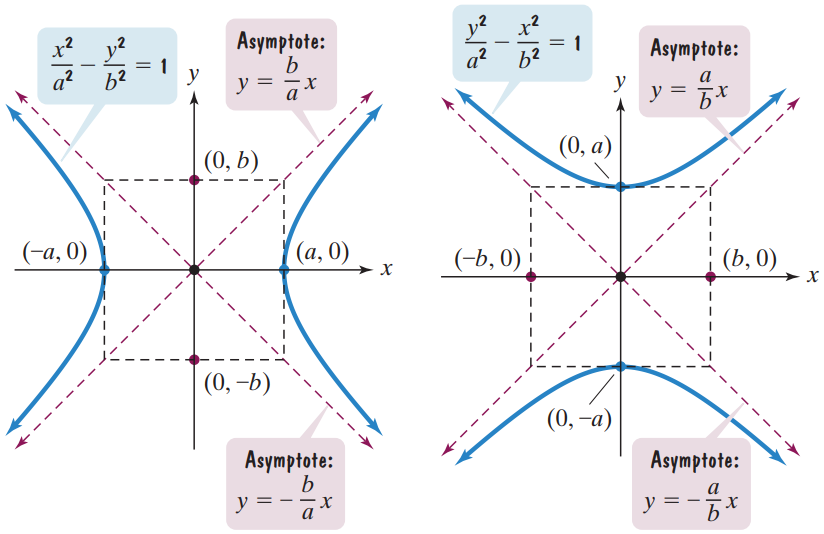
\includegraphics[width=0.8\textwidth,keepaspectratio]{figs/HyperbolaGraphs.png}
\end{center}

\begin{definition}
    A horizontal or oblique \textbf{asymptote} of a graph is a line with the property that the distance from the line to points on the graph approaches 0 as $x\to-\infty$ or as $x\to\infty$.
\end{definition}

A parabola has two asymptotes which are intersect at the center and symmetric with respect to the center or each axis.

\begin{proposition}[Characterization of hyperbola by asymptotes]
    A hyperbola has an equation $\dfrac{x^2}{a^2}-\dfrac{y^2}{b^2}=k$ if and only if its asymptotes are $y=\pm\dfrac{b}{a}x$ where $k$ is a non-zero real number.
\end{proposition}

The rectangle whose diagonals are along the aymptotes and with one side passing through a vertex of a hyperbola is called the \textbf{central box}.

The line segment through the center, perpendicular to the transverse axis with endpoints on the the central rectangle is the \textbf{conjugate axis}.

\begin{center}
    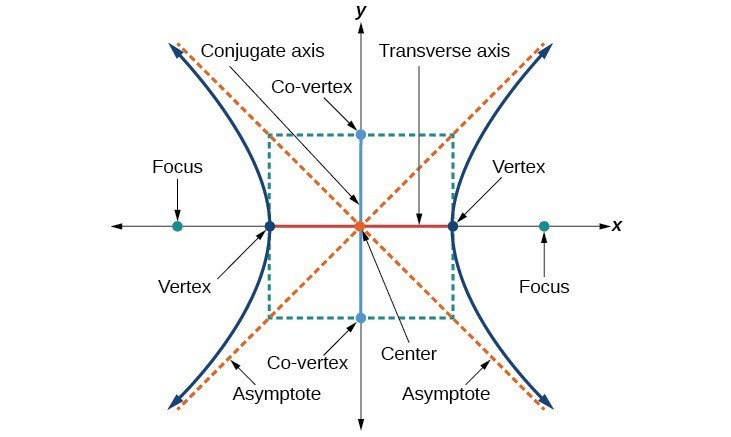
\includegraphics[width=0.7\textwidth,keepaspectratio]{figs/KeyConceptsOfHyperbola.jpg}
\end{center}

\begin{example}
    A hyperbola has the equation $9x^2-16y^2=121$.
    Find the vertices, foci, length of the transverse axis, and asymptotes. Sketch the graph.
\end{example}
\vspace*{8\baselineskip}

\begin{example}
    Find the vertices, foci, length of the transverse axis, and asymptotes of the hyperbola $x^2-9y^2+9=0$. Sketch the graph.
\end{example}
\vspace*{8\baselineskip}

\begin{example}
    Find the equation of the hyperbola with vertices $(\pm 3, 0)$ and foci $(\pm 4, 0)$.
\end{example}
\vspace*{8\baselineskip}

\begin{example}
    Find the equation and the foci of the hyperbola with vertices $(0,\pm 2)$ and asymptotes $y=\pm2x$.
\end{example}
\vspace*{8\baselineskip}

\section*{Practice}

\begin{exercise}
    Find the vertex, focus, and directrix of the parabola. Sketch the graph.\\
    \begin{enumerate*}
        \item $x^2=-8y$.
        \item $y^2=12x$.
        \item $x^2+6y=0$.
        \item $2x-y^2=0$.
    \end{enumerate*}
\end{exercise}
\vspace*{10\baselineskip}

\begin{exercise}
    An equation of an ellipse is given. Find the center, vertices, and foci of the ellipse, and the lengths of the major and minor axes. Sketch the graph.\\
    \begin{enumerate*}
        \item $\dfrac{x^2}{9}+\dfrac{y^2}{25}=1$.
        \item $\dfrac{y^2}{9}+\dfrac{x^2}{25}=1$.
        \item $9x^2+25y^2=1$.
        \item $25x^2+9y^2-16=0$.
    \end{enumerate*}
\end{exercise}
\vspace*{10\baselineskip}

\begin{exercise}
    An equation of an ellipse is given. Find the center, vertices, foci, and asymptotes of the hyperbola. Sketch the graph.\\
    \begin{enumerate*}
        \item $\dfrac{x^2}{9}-\dfrac{y^2}{25}=1$.
        \item $\dfrac{y^2}{9}-\dfrac{x^2}{25}=1$.
        \item $9x^2-25y^2=1$.
        \item $25x^2-9y^2-4=0$.
    \end{enumerate*}
\end{exercise}
\vspace*{10\baselineskip}

\begin{exercise}
    Find an equation for
    the conic section with the given properties.
    \begin{enumerate}
        \item The parabola with vertex at the origin and focus $(0, 5)$.
        \item The parabola with vertex at the origin and the directrix $x=-2$.
        \item The ellipse with vertices $(\pm 2, 0)$ and foci $(\pm 1, 0)$.
        \item the ellipse with foci $(0,\pm 3)$ and the eccentricity $e=\frac34$.
        \item The hyperbola with foci $(0,\pm 3)$ and vertices $(\pm 2, 0)$.
        \item The hyperbola with foci $(\pm 5, 0)$ and asymptotes $y=\pm\frac34$.
    \end{enumerate}
\end{exercise}

\begin{exercise}
    Find an question for the conic section with the given graph.
    \begin{enumerate}
        \item \mbox{}

        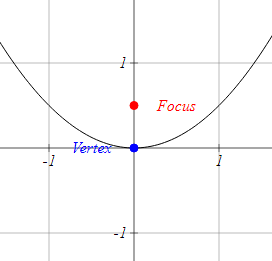
\includegraphics[width=0.3\textwidth]{figs/ParabolaEqFromGraph.png}
        \item \mbox{}

        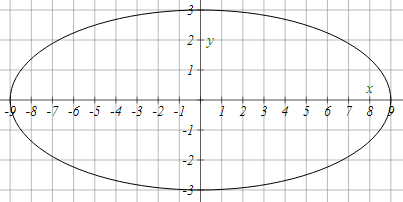
\includegraphics[width=0.4\textwidth]{figs/EllipseEqFromGraph.png}
        \item\mbox{}

        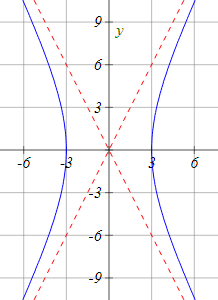
\includegraphics[width=0.3\textwidth]{figs/HyperbolaEqFromGraph.png}
    \end{enumerate}
\end{exercise}


\newlecture
% !TeX root =  main.tex

\section{Functions}


\begin{definition}[Function]

    A parabola is the set of all points in the plane that are equidistant from a fixed point $F$ (called the \textbf{focus}) and a fixed line $l$ (called the \textbf{directrix}).
\end{definition}
\begin{wrapfigure}[10]{r}{0.4\textwidth}
    \centering
    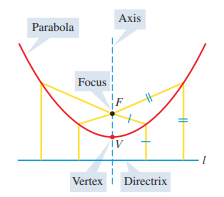
\includegraphics[width=0.3\textwidth,keepaspectratio]{figs/parabola-concepts.png}
\end{wrapfigure}
The \textbf{axis of symmetry} is the line that runs through the focus perpendicular to the directrix. The \textbf{vertex} $V$ is the intersection of the parabola and the axis of symmetry. Equivalently, the vertex lies halfway between the focus and the directrix.

\begin{theorem}[Parabola with vertical axis]
    A parabola has an equation $x^2=4py$ if and only if two of the following properties are satisfied:
    \begin{enumerate}[sepno]
        \item the vertex is $V(0, 0)$;
        \item the focus is $F(0, p)$;
        \item the directrix is $y=-p$.
    \end{enumerate}

    The parabola opens upward if $p>0$ or downward if $p<0$.
\end{theorem}

\begin{theorem}[Parabola with horizontal axis]
    A parabola has an equation $y^2=4px$ if and only if two of the following properties are satisfied:
    \begin{enumerate}[sepno]
        \item the vertex is $V(0, 0)$;
        \item the focus is $F(p, 0)$;
        \item the directrix is $x=-p$.
    \end{enumerate}

    The parabola opens to the right if $p>0$ or to the left if $p<0$.
\end{theorem}
\begin{center}
    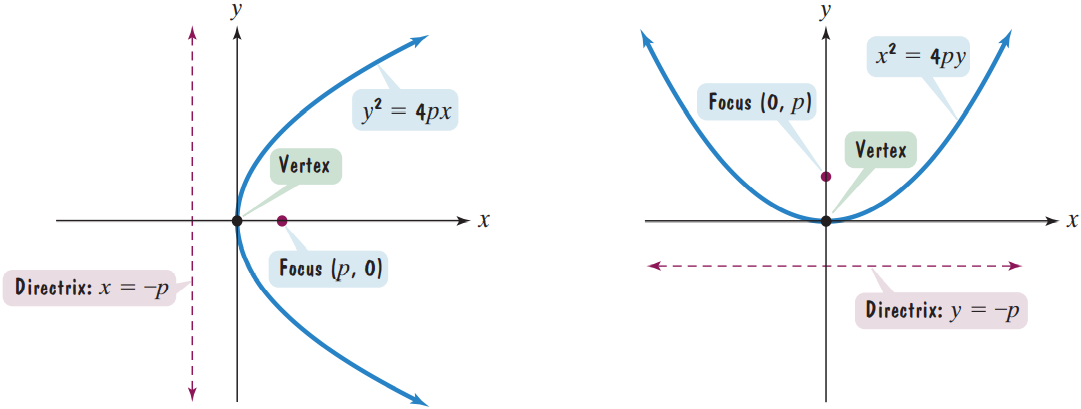
\includegraphics[width=0.8\textwidth,keepaspectratio]{figs/ParabolaGraphs.png}
\end{center}
The equations in the above theorems are called the standard form of the equation of a parabola with its vertex at the origin.

\begin{example}
    Find an equation of the parabola with the vertex $V(0,0)$ and focus $F(0,2)$.
\end{example}
\begin{solution}
    Because the vertex is $V(0, 0)$ and the focus is $F(0, 2)$. We know that $p=2$ and the axis of symmetry is vertical. Therefore, the parabola is defined by $x^2=8y$ by the theorem.
\end{solution}

\begin{example}
    Find the focus and directrix of the parabola $y=-x^2$.
\end{example}
\begin{solution}
    The equation of the parabola can be written as $x^2=-y$. Comparing with the standard form equation $x^2=4py$, we see that $4p=-1$ which implies $p=-\frac14$. So the focus is $\left(0, -\frac14\right)$ and the directrix is $y=-\left(-\frac14\right)$ which simplifies into $y=\frac{1}{4}$.
\end{solution}

The line segment that runs through the focus perpendicular to the
axis, with endpoints on the parabola, is called the \textbf{latus rectum}, and its length is the \textbf{focal diameter} of the parabola.

Because the latus rectum is parallel to the directrix and points on a parabola are equidistant from the focus and the directrix. The focal diameter equals the distance from the focus to the directrix. In particular, for a parabola with the vertex at the origin and the focus on a coordinate axis, the focal diameter is $|4p|$.

\begin{example}
    Find the focus, directrix, and focal diameter of the parabola $y=\frac{1}{2}x^2$.
\end{example}
\begin{solution}
    Rewriting the equation into standard form yields $x^2=2y$. Then $4p=2$ and $p=\frac{1}{2}$. Since the axis of symmetry is vertical, the focus is $(0, \frac12)$, the directrix is $y=-\frac12$, and the focal diameter is $|4p|=4\cdot\frac12=2$.
\end{solution}

\begin{example}
    A searchlight has a parabolic reflector that forms a “bowl,” which is 12 in. wide from rim to rim and 8 in. deep.  If the filament of the light bulb is located at the focus, how far from the vertex of the reflector is it?
\end{example}
\vspace{-2\baselineskip}
\begin{center}
    \noindent
    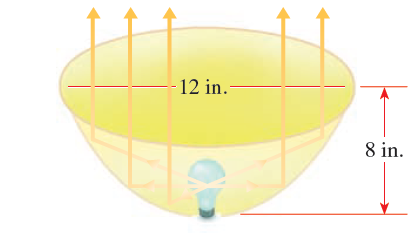
\includegraphics[height=8\baselineskip,keepaspectratio]{figs/SearchlightReflector1.png}
    \hspace{2em}
    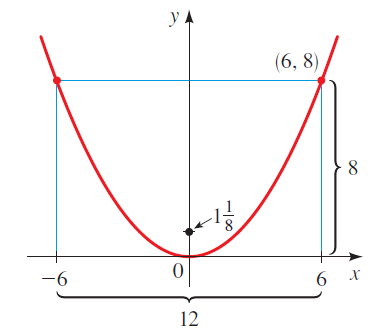
\includegraphics[height=9\baselineskip,keepaspectratio]{figs/SearchlightReflector2.png}
\end{center}

\begin{solution}
    We may assume the vertex is at the origin and the light bulb is at $F(0, p)$.
    Since the reflector is parabolic, that is the vertical section through the vertex and the light bulb is a parabola, an equation of the parabola is $x^2=4py$.
    Because the parabola is symmetric with respect to the axis of symmetry which is the vertical line passing through the vertex and the focus, there is a point $(6,8)$ on the parabola. It then follows that
    \[6^2=4p\cdot 8.\]
    Solving for $p$ yields $p=\frac{9}{8}$. So the light bulb is $\frac{9}{8}$ in. above the vertex of the reflector.
\end{solution}

\section{Ellipses}

\begin{definition}[Geometric Definition of an Ellipse]
    An \textbf{ellipse} is the set of all points in the plane the sum of whose distances from two fixed points $F_1$ and $F_2$ is a constant. These two fixed points are the \textbf{foci} (plural of focus) of the ellipse.
\end{definition}

\begin{definition}
    The midpoint of the line segment joining the foci is called the \textbf{center} of the ellipse.

    The line segment through the foci with endpoints on the ellipse is called the \textbf{major axis}

    The line segment perpendicular to the major axis through the center with endpoints on the ellipse is the \textbf{minor axis}.

    The intersections of the ellipse and the major axis are called the \textbf{vertices} of the ellipse.

    The distance of the foci to the center is called the \textbf{focal distance} or \textbf{linear eccentricity}.

\end{definition}

\begin{proposition}
    Suppose the length of the major axis is $2a$, the length of the minor axis is $2b$, and the linear eccentricity is $c$. Then
    \[a^2=b^2+c^2.\]
\end{proposition}

\begin{theorem}[Ellipse centered at the origin and with the major axis along the $x$-axis]
An ellipse has an equation $\frac{x^2}{a^2}+\frac{y^2}{b^2}=1$ if and only if the foci are $(\pm \sqrt{a^2-b^2}, 0)$ and the vertices are $(\pm a, 0)$, where $a>0$.
\end{theorem}

\begin{theorem}[Ellipse centered at the origin and with the major axis along the $y$-axis]
An ellipse has an equation $\frac{x^2}{b^2}+\frac{y^2}{a^2}=1$ if and only if the foci are $(0, \pm \sqrt{a^2-b^2})$ and the vertices are $(0, \pm a)$, where $a>0$.
\end{theorem}

\begin{center}
    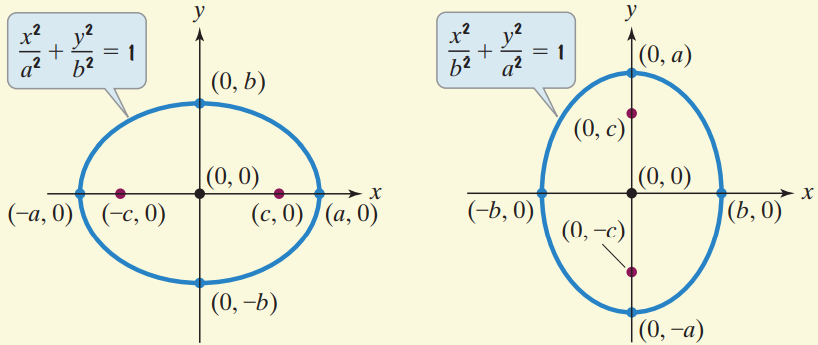
\includegraphics[width=0.8\textwidth,keepaspectratio]{figs/EllipseGraphs.png}
\end{center}

The questions of ellipses in the above theorems are called the \textbf{standard form}.

\begin{example}
    An ellipse has the equation $\dfrac{x^2}{9}+\dfrac{y^2}{4}=1$.
    Find the foci, the vertices, and the lengths of the major and minor axes. Sketch the graph.
\end{example}
\vspace*{6\baselineskip}

\begin{example}
    Find the foci of the ellipse $16x^2+9y^2=144$.
\end{example}
\vspace*{6\baselineskip}

\begin{example}
    Find an equation of the ellipse with the vertices $(\pm 4, 0)$ and the foci $(\pm 2, 0)$.
\end{example}
\vspace*{6\baselineskip}

\begin{definition}
    The eccentricity $e$ of an ellipse is defined as
    \[e=\dfrac{\text{focal distance}}{\frac12\left(\text{length of the major axis}\right)}.\]
    \begin{center}
        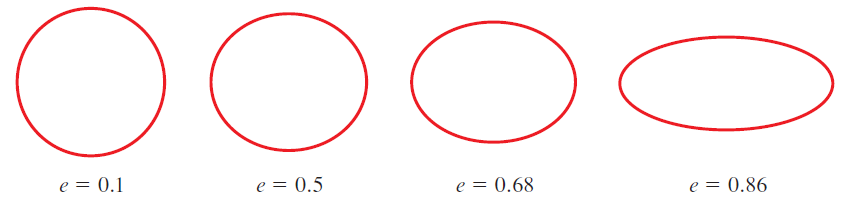
\includegraphics[scale=0.8]{figs/EllipseWithVariousEccentricities.png}
    \end{center}
\end{definition}

For an ellipse centered at the origin and with the major axis along a coordinate axis, the eccentricity is $e=\dfrac ca$.

\begin{example}
    Find the equation of the ellipse with foci $(0, \pm8)$ and the eccentricity $e=\frac45$.
\end{example}
\vspace*{8\baselineskip}

\section{Hyperbola}

\begin{definition}[Geometric Definition of a Hyperbola]
    A \textbf{hyperbola} is the set of all points in the plane, the difference of whose distances
    from two fixed points $F_1$ and $F_2$ is a constant. These two
    fixed points are the \textbf{foci} of the hyperbola.
\end{definition}

\begin{definition}
    The line segment containing the foci with endpoints on the hyperbola is called the \textbf{transverse axis}.

    The endpoints of the transverse axis are called the \textbf{vertices} of the hyperbola.

    The midpoint of the line segment joining the foci is the \textbf{center} of the hyperbola.

    The distance of the foci to the center is called the \textbf{focal distance} or \textbf{linear eccentricity}.

    The hyperbola consists of two separate curves, called \textbf{branches}, that are symmetric with respect to the transverse axis, conjugate
    axis, and center. \end{definition}


\begin{theorem}[Hyperbola centered at the origin and with the transverse axis along the $x$-axis]
A hyperbola has an equation $\frac{x^2}{a^2}-\frac{y^2}{b^2}=1$ if and only if the foci are $(\pm \sqrt{a^2+b^2}, 0)$ and the vertices are $(\pm a, 0)$.
\end{theorem}

\begin{theorem}[Hyperbola centered at the origin and with the transverse axis along the $y$-axis]
A hyperbola has an equation $\frac{x^2}{b^2}-\frac{y^2}{a^2}=1$ if and only if the foci are $(0, \pm \sqrt{a^2+b^2})$ and the vertices are $(0, \pm a)$.
\end{theorem}

\begin{center}
    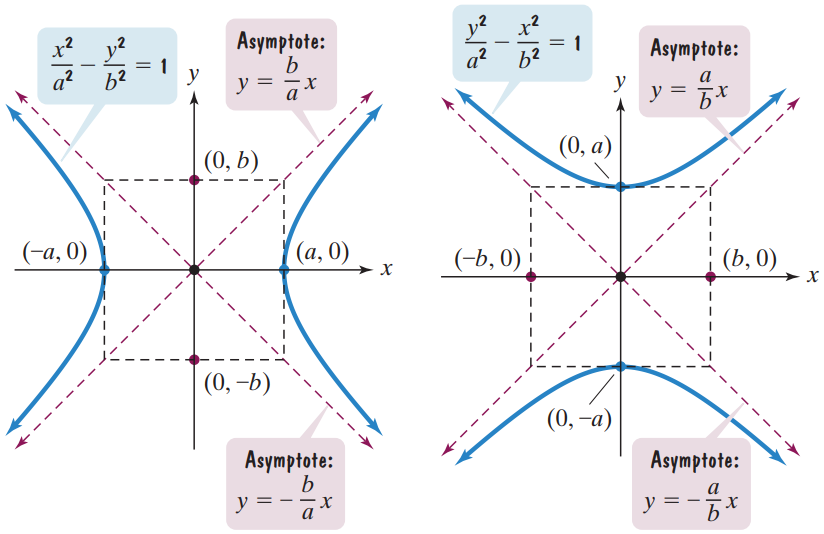
\includegraphics[width=0.8\textwidth,keepaspectratio]{figs/HyperbolaGraphs.png}
\end{center}

\begin{definition}
    A horizontal or oblique \textbf{asymptote} of a graph is a line with the property that the distance from the line to points on the graph approaches 0 as $x\to-\infty$ or as $x\to\infty$.
\end{definition}

A parabola has two asymptotes which are intersect at the center and symmetric with respect to the center or each axis.

\begin{proposition}[Characterization of hyperbola by asymptotes]
    A hyperbola has an equation $\dfrac{x^2}{a^2}-\dfrac{y^2}{b^2}=k$ if and only if its asymptotes are $y=\pm\dfrac{b}{a}x$ where $k$ is a non-zero real number.
\end{proposition}

The rectangle whose diagonals are along the aymptotes and with one side passing through a vertex of a hyperbola is called the \textbf{central box}.

The line segment through the center, perpendicular to the transverse axis with endpoints on the the central rectangle is the \textbf{conjugate axis}.

\begin{center}
    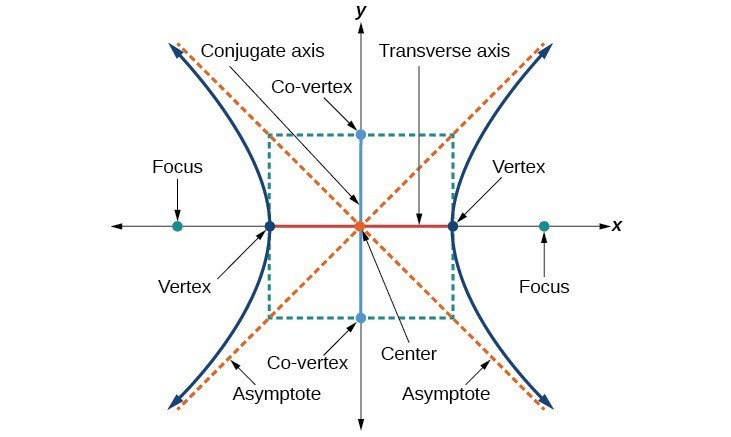
\includegraphics[width=0.7\textwidth,keepaspectratio]{figs/KeyConceptsOfHyperbola.jpg}
\end{center}

\begin{example}
    A hyperbola has the equation $9x^2-16y^2=121$.
    Find the vertices, foci, length of the transverse axis, and asymptotes. Sketch the graph.
\end{example}
\vspace*{8\baselineskip}

\begin{example}
    Find the vertices, foci, length of the transverse axis, and asymptotes of the hyperbola $x^2-9y^2+9=0$. Sketch the graph.
\end{example}
\vspace*{8\baselineskip}

\begin{example}
    Find the equation of the hyperbola with vertices $(\pm 3, 0)$ and foci $(\pm 4, 0)$.
\end{example}
\vspace*{8\baselineskip}

\begin{example}
    Find the equation and the foci of the hyperbola with vertices $(0,\pm 2)$ and asymptotes $y=\pm2x$.
\end{example}
\vspace*{8\baselineskip}

\section*{Practice}

\begin{exercise}
    Find the vertex, focus, and directrix of the parabola. Sketch the graph.\\
    \begin{enumerate*}
        \item $x^2=-8y$.
        \item $y^2=12x$.
        \item $x^2+6y=0$.
        \item $2x-y^2=0$.
    \end{enumerate*}
\end{exercise}
\vspace*{10\baselineskip}

\begin{exercise}
    An equation of an ellipse is given. Find the center, vertices, and foci of the ellipse, and the lengths of the major and minor axes. Sketch the graph.\\
    \begin{enumerate*}
        \item $\dfrac{x^2}{9}+\dfrac{y^2}{25}=1$.
        \item $\dfrac{y^2}{9}+\dfrac{x^2}{25}=1$.
        \item $9x^2+25y^2=1$.
        \item $25x^2+9y^2-16=0$.
    \end{enumerate*}
\end{exercise}
\vspace*{10\baselineskip}

\begin{exercise}
    An equation of an ellipse is given. Find the center, vertices, foci, and asymptotes of the hyperbola. Sketch the graph.\\
    \begin{enumerate*}
        \item $\dfrac{x^2}{9}-\dfrac{y^2}{25}=1$.
        \item $\dfrac{y^2}{9}-\dfrac{x^2}{25}=1$.
        \item $9x^2-25y^2=1$.
        \item $25x^2-9y^2-4=0$.
    \end{enumerate*}
\end{exercise}
\vspace*{10\baselineskip}

\begin{exercise}
    Find an equation for
    the conic section with the given properties.
    \begin{enumerate}
        \item The parabola with vertex at the origin and focus $(0, 5)$.
        \item The parabola with vertex at the origin and the directrix $x=-2$.
        \item The ellipse with vertices $(\pm 2, 0)$ and foci $(\pm 1, 0)$.
        \item the ellipse with foci $(0,\pm 3)$ and the eccentricity $e=\frac34$.
        \item The hyperbola with foci $(0,\pm 3)$ and vertices $(\pm 2, 0)$.
        \item The hyperbola with foci $(\pm 5, 0)$ and asymptotes $y=\pm\frac34$.
    \end{enumerate}
\end{exercise}

\begin{exercise}
    Find an question for the conic section with the given graph.
    \begin{enumerate}
        \item \mbox{}

        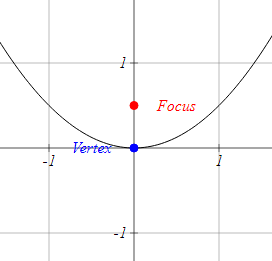
\includegraphics[width=0.3\textwidth]{figs/ParabolaEqFromGraph.png}
        \item \mbox{}

        \includegraphics[width=0.4\textwidth]{figs/EllipseEqFromGraph.png}
        \item\mbox{}

        \includegraphics[width=0.3\textwidth]{figs/HyperbolaEqFromGraph.png}
    \end{enumerate}
\end{exercise}


\newlecture
% !TeX root =  main.tex

\section{Functions}


\begin{definition}[Function]

    A parabola is the set of all points in the plane that are equidistant from a fixed point $F$ (called the \textbf{focus}) and a fixed line $l$ (called the \textbf{directrix}).
\end{definition}
\begin{wrapfigure}[10]{r}{0.4\textwidth}
    \centering
    \includegraphics[width=0.3\textwidth,keepaspectratio]{figs/parabola-concepts.png}
\end{wrapfigure}
The \textbf{axis of symmetry} is the line that runs through the focus perpendicular to the directrix. The \textbf{vertex} $V$ is the intersection of the parabola and the axis of symmetry. Equivalently, the vertex lies halfway between the focus and the directrix.

\begin{theorem}[Parabola with vertical axis]
    A parabola has an equation $x^2=4py$ if and only if two of the following properties are satisfied:
    \begin{enumerate}[sepno]
        \item the vertex is $V(0, 0)$;
        \item the focus is $F(0, p)$;
        \item the directrix is $y=-p$.
    \end{enumerate}

    The parabola opens upward if $p>0$ or downward if $p<0$.
\end{theorem}

\begin{theorem}[Parabola with horizontal axis]
    A parabola has an equation $y^2=4px$ if and only if two of the following properties are satisfied:
    \begin{enumerate}[sepno]
        \item the vertex is $V(0, 0)$;
        \item the focus is $F(p, 0)$;
        \item the directrix is $x=-p$.
    \end{enumerate}

    The parabola opens to the right if $p>0$ or to the left if $p<0$.
\end{theorem}
\begin{center}
    \includegraphics[width=0.8\textwidth,keepaspectratio]{figs/ParabolaGraphs.png}
\end{center}
The equations in the above theorems are called the standard form of the equation of a parabola with its vertex at the origin.

\begin{example}
    Find an equation of the parabola with the vertex $V(0,0)$ and focus $F(0,2)$.
\end{example}
\begin{solution}
    Because the vertex is $V(0, 0)$ and the focus is $F(0, 2)$. We know that $p=2$ and the axis of symmetry is vertical. Therefore, the parabola is defined by $x^2=8y$ by the theorem.
\end{solution}

\begin{example}
    Find the focus and directrix of the parabola $y=-x^2$.
\end{example}
\begin{solution}
    The equation of the parabola can be written as $x^2=-y$. Comparing with the standard form equation $x^2=4py$, we see that $4p=-1$ which implies $p=-\frac14$. So the focus is $\left(0, -\frac14\right)$ and the directrix is $y=-\left(-\frac14\right)$ which simplifies into $y=\frac{1}{4}$.
\end{solution}

The line segment that runs through the focus perpendicular to the
axis, with endpoints on the parabola, is called the \textbf{latus rectum}, and its length is the \textbf{focal diameter} of the parabola.

Because the latus rectum is parallel to the directrix and points on a parabola are equidistant from the focus and the directrix. The focal diameter equals the distance from the focus to the directrix. In particular, for a parabola with the vertex at the origin and the focus on a coordinate axis, the focal diameter is $|4p|$.

\begin{example}
    Find the focus, directrix, and focal diameter of the parabola $y=\frac{1}{2}x^2$.
\end{example}
\begin{solution}
    Rewriting the equation into standard form yields $x^2=2y$. Then $4p=2$ and $p=\frac{1}{2}$. Since the axis of symmetry is vertical, the focus is $(0, \frac12)$, the directrix is $y=-\frac12$, and the focal diameter is $|4p|=4\cdot\frac12=2$.
\end{solution}

\begin{example}
    A searchlight has a parabolic reflector that forms a “bowl,” which is 12 in. wide from rim to rim and 8 in. deep.  If the filament of the light bulb is located at the focus, how far from the vertex of the reflector is it?
\end{example}
\vspace{-2\baselineskip}
\begin{center}
    \noindent
    \includegraphics[height=8\baselineskip,keepaspectratio]{figs/SearchlightReflector1.png}
    \hspace{2em}
    \includegraphics[height=9\baselineskip,keepaspectratio]{figs/SearchlightReflector2.png}
\end{center}

\begin{solution}
    We may assume the vertex is at the origin and the light bulb is at $F(0, p)$.
    Since the reflector is parabolic, that is the vertical section through the vertex and the light bulb is a parabola, an equation of the parabola is $x^2=4py$.
    Because the parabola is symmetric with respect to the axis of symmetry which is the vertical line passing through the vertex and the focus, there is a point $(6,8)$ on the parabola. It then follows that
    \[6^2=4p\cdot 8.\]
    Solving for $p$ yields $p=\frac{9}{8}$. So the light bulb is $\frac{9}{8}$ in. above the vertex of the reflector.
\end{solution}

\section{Ellipses}

\begin{definition}[Geometric Definition of an Ellipse]
    An \textbf{ellipse} is the set of all points in the plane the sum of whose distances from two fixed points $F_1$ and $F_2$ is a constant. These two fixed points are the \textbf{foci} (plural of focus) of the ellipse.
\end{definition}

\begin{definition}
    The midpoint of the line segment joining the foci is called the \textbf{center} of the ellipse.

    The line segment through the foci with endpoints on the ellipse is called the \textbf{major axis}

    The line segment perpendicular to the major axis through the center with endpoints on the ellipse is the \textbf{minor axis}.

    The intersections of the ellipse and the major axis are called the \textbf{vertices} of the ellipse.

    The distance of the foci to the center is called the \textbf{focal distance} or \textbf{linear eccentricity}.

\end{definition}

\begin{proposition}
    Suppose the length of the major axis is $2a$, the length of the minor axis is $2b$, and the linear eccentricity is $c$. Then
    \[a^2=b^2+c^2.\]
\end{proposition}

\begin{theorem}[Ellipse centered at the origin and with the major axis along the $x$-axis]
An ellipse has an equation $\frac{x^2}{a^2}+\frac{y^2}{b^2}=1$ if and only if the foci are $(\pm \sqrt{a^2-b^2}, 0)$ and the vertices are $(\pm a, 0)$, where $a>0$.
\end{theorem}

\begin{theorem}[Ellipse centered at the origin and with the major axis along the $y$-axis]
An ellipse has an equation $\frac{x^2}{b^2}+\frac{y^2}{a^2}=1$ if and only if the foci are $(0, \pm \sqrt{a^2-b^2})$ and the vertices are $(0, \pm a)$, where $a>0$.
\end{theorem}

\begin{center}
    \includegraphics[width=0.8\textwidth,keepaspectratio]{figs/EllipseGraphs.png}
\end{center}

The questions of ellipses in the above theorems are called the \textbf{standard form}.

\begin{example}
    An ellipse has the equation $\dfrac{x^2}{9}+\dfrac{y^2}{4}=1$.
    Find the foci, the vertices, and the lengths of the major and minor axes. Sketch the graph.
\end{example}
\vspace*{6\baselineskip}

\begin{example}
    Find the foci of the ellipse $16x^2+9y^2=144$.
\end{example}
\vspace*{6\baselineskip}

\begin{example}
    Find an equation of the ellipse with the vertices $(\pm 4, 0)$ and the foci $(\pm 2, 0)$.
\end{example}
\vspace*{6\baselineskip}

\begin{definition}
    The eccentricity $e$ of an ellipse is defined as
    \[e=\dfrac{\text{focal distance}}{\frac12\left(\text{length of the major axis}\right)}.\]
    \begin{center}
        \includegraphics[scale=0.8]{figs/EllipseWithVariousEccentricities.png}
    \end{center}
\end{definition}

For an ellipse centered at the origin and with the major axis along a coordinate axis, the eccentricity is $e=\dfrac ca$.

\begin{example}
    Find the equation of the ellipse with foci $(0, \pm8)$ and the eccentricity $e=\frac45$.
\end{example}
\vspace*{8\baselineskip}

\section{Hyperbola}

\begin{definition}[Geometric Definition of a Hyperbola]
    A \textbf{hyperbola} is the set of all points in the plane, the difference of whose distances
    from two fixed points $F_1$ and $F_2$ is a constant. These two
    fixed points are the \textbf{foci} of the hyperbola.
\end{definition}

\begin{definition}
    The line segment containing the foci with endpoints on the hyperbola is called the \textbf{transverse axis}.

    The endpoints of the transverse axis are called the \textbf{vertices} of the hyperbola.

    The midpoint of the line segment joining the foci is the \textbf{center} of the hyperbola.

    The distance of the foci to the center is called the \textbf{focal distance} or \textbf{linear eccentricity}.

    The hyperbola consists of two separate curves, called \textbf{branches}, that are symmetric with respect to the transverse axis, conjugate
    axis, and center. \end{definition}


\begin{theorem}[Hyperbola centered at the origin and with the transverse axis along the $x$-axis]
A hyperbola has an equation $\frac{x^2}{a^2}-\frac{y^2}{b^2}=1$ if and only if the foci are $(\pm \sqrt{a^2+b^2}, 0)$ and the vertices are $(\pm a, 0)$.
\end{theorem}

\begin{theorem}[Hyperbola centered at the origin and with the transverse axis along the $y$-axis]
A hyperbola has an equation $\frac{x^2}{b^2}-\frac{y^2}{a^2}=1$ if and only if the foci are $(0, \pm \sqrt{a^2+b^2})$ and the vertices are $(0, \pm a)$.
\end{theorem}

\begin{center}
    \includegraphics[width=0.8\textwidth,keepaspectratio]{figs/HyperbolaGraphs.png}
\end{center}

\begin{definition}
    A horizontal or oblique \textbf{asymptote} of a graph is a line with the property that the distance from the line to points on the graph approaches 0 as $x\to-\infty$ or as $x\to\infty$.
\end{definition}

A parabola has two asymptotes which are intersect at the center and symmetric with respect to the center or each axis.

\begin{proposition}[Characterization of hyperbola by asymptotes]
    A hyperbola has an equation $\dfrac{x^2}{a^2}-\dfrac{y^2}{b^2}=k$ if and only if its asymptotes are $y=\pm\dfrac{b}{a}x$ where $k$ is a non-zero real number.
\end{proposition}

The rectangle whose diagonals are along the aymptotes and with one side passing through a vertex of a hyperbola is called the \textbf{central box}.

The line segment through the center, perpendicular to the transverse axis with endpoints on the the central rectangle is the \textbf{conjugate axis}.

\begin{center}
    \includegraphics[width=0.7\textwidth,keepaspectratio]{figs/KeyConceptsOfHyperbola.jpg}
\end{center}

\begin{example}
    A hyperbola has the equation $9x^2-16y^2=121$.
    Find the vertices, foci, length of the transverse axis, and asymptotes. Sketch the graph.
\end{example}
\vspace*{8\baselineskip}

\begin{example}
    Find the vertices, foci, length of the transverse axis, and asymptotes of the hyperbola $x^2-9y^2+9=0$. Sketch the graph.
\end{example}
\vspace*{8\baselineskip}

\begin{example}
    Find the equation of the hyperbola with vertices $(\pm 3, 0)$ and foci $(\pm 4, 0)$.
\end{example}
\vspace*{8\baselineskip}

\begin{example}
    Find the equation and the foci of the hyperbola with vertices $(0,\pm 2)$ and asymptotes $y=\pm2x$.
\end{example}
\vspace*{8\baselineskip}

\section*{Practice}

\begin{exercise}
    Find the vertex, focus, and directrix of the parabola. Sketch the graph.\\
    \begin{enumerate*}
        \item $x^2=-8y$.
        \item $y^2=12x$.
        \item $x^2+6y=0$.
        \item $2x-y^2=0$.
    \end{enumerate*}
\end{exercise}
\vspace*{10\baselineskip}

\begin{exercise}
    An equation of an ellipse is given. Find the center, vertices, and foci of the ellipse, and the lengths of the major and minor axes. Sketch the graph.\\
    \begin{enumerate*}
        \item $\dfrac{x^2}{9}+\dfrac{y^2}{25}=1$.
        \item $\dfrac{y^2}{9}+\dfrac{x^2}{25}=1$.
        \item $9x^2+25y^2=1$.
        \item $25x^2+9y^2-16=0$.
    \end{enumerate*}
\end{exercise}
\vspace*{10\baselineskip}

\begin{exercise}
    An equation of an ellipse is given. Find the center, vertices, foci, and asymptotes of the hyperbola. Sketch the graph.\\
    \begin{enumerate*}
        \item $\dfrac{x^2}{9}-\dfrac{y^2}{25}=1$.
        \item $\dfrac{y^2}{9}-\dfrac{x^2}{25}=1$.
        \item $9x^2-25y^2=1$.
        \item $25x^2-9y^2-4=0$.
    \end{enumerate*}
\end{exercise}
\vspace*{10\baselineskip}

\begin{exercise}
    Find an equation for
    the conic section with the given properties.
    \begin{enumerate}
        \item The parabola with vertex at the origin and focus $(0, 5)$.
        \item The parabola with vertex at the origin and the directrix $x=-2$.
        \item The ellipse with vertices $(\pm 2, 0)$ and foci $(\pm 1, 0)$.
        \item the ellipse with foci $(0,\pm 3)$ and the eccentricity $e=\frac34$.
        \item The hyperbola with foci $(0,\pm 3)$ and vertices $(\pm 2, 0)$.
        \item The hyperbola with foci $(\pm 5, 0)$ and asymptotes $y=\pm\frac34$.
    \end{enumerate}
\end{exercise}

\begin{exercise}
    Find an question for the conic section with the given graph.
    \begin{enumerate}
        \item \mbox{}

        \includegraphics[width=0.3\textwidth]{figs/ParabolaEqFromGraph.png}
        \item \mbox{}

        \includegraphics[width=0.4\textwidth]{figs/EllipseEqFromGraph.png}
        \item\mbox{}

        \includegraphics[width=0.3\textwidth]{figs/HyperbolaEqFromGraph.png}
    \end{enumerate}
\end{exercise}


\newlecture
% !TeX root =  main.tex

\section{Functions}


\begin{definition}[Function]

    A parabola is the set of all points in the plane that are equidistant from a fixed point $F$ (called the \textbf{focus}) and a fixed line $l$ (called the \textbf{directrix}).
\end{definition}
\begin{wrapfigure}[10]{r}{0.4\textwidth}
    \centering
    \includegraphics[width=0.3\textwidth,keepaspectratio]{figs/parabola-concepts.png}
\end{wrapfigure}
The \textbf{axis of symmetry} is the line that runs through the focus perpendicular to the directrix. The \textbf{vertex} $V$ is the intersection of the parabola and the axis of symmetry. Equivalently, the vertex lies halfway between the focus and the directrix.

\begin{theorem}[Parabola with vertical axis]
    A parabola has an equation $x^2=4py$ if and only if two of the following properties are satisfied:
    \begin{enumerate}[sepno]
        \item the vertex is $V(0, 0)$;
        \item the focus is $F(0, p)$;
        \item the directrix is $y=-p$.
    \end{enumerate}

    The parabola opens upward if $p>0$ or downward if $p<0$.
\end{theorem}

\begin{theorem}[Parabola with horizontal axis]
    A parabola has an equation $y^2=4px$ if and only if two of the following properties are satisfied:
    \begin{enumerate}[sepno]
        \item the vertex is $V(0, 0)$;
        \item the focus is $F(p, 0)$;
        \item the directrix is $x=-p$.
    \end{enumerate}

    The parabola opens to the right if $p>0$ or to the left if $p<0$.
\end{theorem}
\begin{center}
    \includegraphics[width=0.8\textwidth,keepaspectratio]{figs/ParabolaGraphs.png}
\end{center}
The equations in the above theorems are called the standard form of the equation of a parabola with its vertex at the origin.

\begin{example}
    Find an equation of the parabola with the vertex $V(0,0)$ and focus $F(0,2)$.
\end{example}
\begin{solution}
    Because the vertex is $V(0, 0)$ and the focus is $F(0, 2)$. We know that $p=2$ and the axis of symmetry is vertical. Therefore, the parabola is defined by $x^2=8y$ by the theorem.
\end{solution}

\begin{example}
    Find the focus and directrix of the parabola $y=-x^2$.
\end{example}
\begin{solution}
    The equation of the parabola can be written as $x^2=-y$. Comparing with the standard form equation $x^2=4py$, we see that $4p=-1$ which implies $p=-\frac14$. So the focus is $\left(0, -\frac14\right)$ and the directrix is $y=-\left(-\frac14\right)$ which simplifies into $y=\frac{1}{4}$.
\end{solution}

The line segment that runs through the focus perpendicular to the
axis, with endpoints on the parabola, is called the \textbf{latus rectum}, and its length is the \textbf{focal diameter} of the parabola.

Because the latus rectum is parallel to the directrix and points on a parabola are equidistant from the focus and the directrix. The focal diameter equals the distance from the focus to the directrix. In particular, for a parabola with the vertex at the origin and the focus on a coordinate axis, the focal diameter is $|4p|$.

\begin{example}
    Find the focus, directrix, and focal diameter of the parabola $y=\frac{1}{2}x^2$.
\end{example}
\begin{solution}
    Rewriting the equation into standard form yields $x^2=2y$. Then $4p=2$ and $p=\frac{1}{2}$. Since the axis of symmetry is vertical, the focus is $(0, \frac12)$, the directrix is $y=-\frac12$, and the focal diameter is $|4p|=4\cdot\frac12=2$.
\end{solution}

\begin{example}
    A searchlight has a parabolic reflector that forms a “bowl,” which is 12 in. wide from rim to rim and 8 in. deep.  If the filament of the light bulb is located at the focus, how far from the vertex of the reflector is it?
\end{example}
\vspace{-2\baselineskip}
\begin{center}
    \noindent
    \includegraphics[height=8\baselineskip,keepaspectratio]{figs/SearchlightReflector1.png}
    \hspace{2em}
    \includegraphics[height=9\baselineskip,keepaspectratio]{figs/SearchlightReflector2.png}
\end{center}

\begin{solution}
    We may assume the vertex is at the origin and the light bulb is at $F(0, p)$.
    Since the reflector is parabolic, that is the vertical section through the vertex and the light bulb is a parabola, an equation of the parabola is $x^2=4py$.
    Because the parabola is symmetric with respect to the axis of symmetry which is the vertical line passing through the vertex and the focus, there is a point $(6,8)$ on the parabola. It then follows that
    \[6^2=4p\cdot 8.\]
    Solving for $p$ yields $p=\frac{9}{8}$. So the light bulb is $\frac{9}{8}$ in. above the vertex of the reflector.
\end{solution}

\section{Ellipses}

\begin{definition}[Geometric Definition of an Ellipse]
    An \textbf{ellipse} is the set of all points in the plane the sum of whose distances from two fixed points $F_1$ and $F_2$ is a constant. These two fixed points are the \textbf{foci} (plural of focus) of the ellipse.
\end{definition}

\begin{definition}
    The midpoint of the line segment joining the foci is called the \textbf{center} of the ellipse.

    The line segment through the foci with endpoints on the ellipse is called the \textbf{major axis}

    The line segment perpendicular to the major axis through the center with endpoints on the ellipse is the \textbf{minor axis}.

    The intersections of the ellipse and the major axis are called the \textbf{vertices} of the ellipse.

    The distance of the foci to the center is called the \textbf{focal distance} or \textbf{linear eccentricity}.

\end{definition}

\begin{proposition}
    Suppose the length of the major axis is $2a$, the length of the minor axis is $2b$, and the linear eccentricity is $c$. Then
    \[a^2=b^2+c^2.\]
\end{proposition}

\begin{theorem}[Ellipse centered at the origin and with the major axis along the $x$-axis]
An ellipse has an equation $\frac{x^2}{a^2}+\frac{y^2}{b^2}=1$ if and only if the foci are $(\pm \sqrt{a^2-b^2}, 0)$ and the vertices are $(\pm a, 0)$, where $a>0$.
\end{theorem}

\begin{theorem}[Ellipse centered at the origin and with the major axis along the $y$-axis]
An ellipse has an equation $\frac{x^2}{b^2}+\frac{y^2}{a^2}=1$ if and only if the foci are $(0, \pm \sqrt{a^2-b^2})$ and the vertices are $(0, \pm a)$, where $a>0$.
\end{theorem}

\begin{center}
    \includegraphics[width=0.8\textwidth,keepaspectratio]{figs/EllipseGraphs.png}
\end{center}

The questions of ellipses in the above theorems are called the \textbf{standard form}.

\begin{example}
    An ellipse has the equation $\dfrac{x^2}{9}+\dfrac{y^2}{4}=1$.
    Find the foci, the vertices, and the lengths of the major and minor axes. Sketch the graph.
\end{example}
\vspace*{6\baselineskip}

\begin{example}
    Find the foci of the ellipse $16x^2+9y^2=144$.
\end{example}
\vspace*{6\baselineskip}

\begin{example}
    Find an equation of the ellipse with the vertices $(\pm 4, 0)$ and the foci $(\pm 2, 0)$.
\end{example}
\vspace*{6\baselineskip}

\begin{definition}
    The eccentricity $e$ of an ellipse is defined as
    \[e=\dfrac{\text{focal distance}}{\frac12\left(\text{length of the major axis}\right)}.\]
    \begin{center}
        \includegraphics[scale=0.8]{figs/EllipseWithVariousEccentricities.png}
    \end{center}
\end{definition}

For an ellipse centered at the origin and with the major axis along a coordinate axis, the eccentricity is $e=\dfrac ca$.

\begin{example}
    Find the equation of the ellipse with foci $(0, \pm8)$ and the eccentricity $e=\frac45$.
\end{example}
\vspace*{8\baselineskip}

\section{Hyperbola}

\begin{definition}[Geometric Definition of a Hyperbola]
    A \textbf{hyperbola} is the set of all points in the plane, the difference of whose distances
    from two fixed points $F_1$ and $F_2$ is a constant. These two
    fixed points are the \textbf{foci} of the hyperbola.
\end{definition}

\begin{definition}
    The line segment containing the foci with endpoints on the hyperbola is called the \textbf{transverse axis}.

    The endpoints of the transverse axis are called the \textbf{vertices} of the hyperbola.

    The midpoint of the line segment joining the foci is the \textbf{center} of the hyperbola.

    The distance of the foci to the center is called the \textbf{focal distance} or \textbf{linear eccentricity}.

    The hyperbola consists of two separate curves, called \textbf{branches}, that are symmetric with respect to the transverse axis, conjugate
    axis, and center. \end{definition}


\begin{theorem}[Hyperbola centered at the origin and with the transverse axis along the $x$-axis]
A hyperbola has an equation $\frac{x^2}{a^2}-\frac{y^2}{b^2}=1$ if and only if the foci are $(\pm \sqrt{a^2+b^2}, 0)$ and the vertices are $(\pm a, 0)$.
\end{theorem}

\begin{theorem}[Hyperbola centered at the origin and with the transverse axis along the $y$-axis]
A hyperbola has an equation $\frac{x^2}{b^2}-\frac{y^2}{a^2}=1$ if and only if the foci are $(0, \pm \sqrt{a^2+b^2})$ and the vertices are $(0, \pm a)$.
\end{theorem}

\begin{center}
    \includegraphics[width=0.8\textwidth,keepaspectratio]{figs/HyperbolaGraphs.png}
\end{center}

\begin{definition}
    A horizontal or oblique \textbf{asymptote} of a graph is a line with the property that the distance from the line to points on the graph approaches 0 as $x\to-\infty$ or as $x\to\infty$.
\end{definition}

A parabola has two asymptotes which are intersect at the center and symmetric with respect to the center or each axis.

\begin{proposition}[Characterization of hyperbola by asymptotes]
    A hyperbola has an equation $\dfrac{x^2}{a^2}-\dfrac{y^2}{b^2}=k$ if and only if its asymptotes are $y=\pm\dfrac{b}{a}x$ where $k$ is a non-zero real number.
\end{proposition}

The rectangle whose diagonals are along the aymptotes and with one side passing through a vertex of a hyperbola is called the \textbf{central box}.

The line segment through the center, perpendicular to the transverse axis with endpoints on the the central rectangle is the \textbf{conjugate axis}.

\begin{center}
    \includegraphics[width=0.7\textwidth,keepaspectratio]{figs/KeyConceptsOfHyperbola.jpg}
\end{center}

\begin{example}
    A hyperbola has the equation $9x^2-16y^2=121$.
    Find the vertices, foci, length of the transverse axis, and asymptotes. Sketch the graph.
\end{example}
\vspace*{8\baselineskip}

\begin{example}
    Find the vertices, foci, length of the transverse axis, and asymptotes of the hyperbola $x^2-9y^2+9=0$. Sketch the graph.
\end{example}
\vspace*{8\baselineskip}

\begin{example}
    Find the equation of the hyperbola with vertices $(\pm 3, 0)$ and foci $(\pm 4, 0)$.
\end{example}
\vspace*{8\baselineskip}

\begin{example}
    Find the equation and the foci of the hyperbola with vertices $(0,\pm 2)$ and asymptotes $y=\pm2x$.
\end{example}
\vspace*{8\baselineskip}

\section*{Practice}

\begin{exercise}
    Find the vertex, focus, and directrix of the parabola. Sketch the graph.\\
    \begin{enumerate*}
        \item $x^2=-8y$.
        \item $y^2=12x$.
        \item $x^2+6y=0$.
        \item $2x-y^2=0$.
    \end{enumerate*}
\end{exercise}
\vspace*{10\baselineskip}

\begin{exercise}
    An equation of an ellipse is given. Find the center, vertices, and foci of the ellipse, and the lengths of the major and minor axes. Sketch the graph.\\
    \begin{enumerate*}
        \item $\dfrac{x^2}{9}+\dfrac{y^2}{25}=1$.
        \item $\dfrac{y^2}{9}+\dfrac{x^2}{25}=1$.
        \item $9x^2+25y^2=1$.
        \item $25x^2+9y^2-16=0$.
    \end{enumerate*}
\end{exercise}
\vspace*{10\baselineskip}

\begin{exercise}
    An equation of an ellipse is given. Find the center, vertices, foci, and asymptotes of the hyperbola. Sketch the graph.\\
    \begin{enumerate*}
        \item $\dfrac{x^2}{9}-\dfrac{y^2}{25}=1$.
        \item $\dfrac{y^2}{9}-\dfrac{x^2}{25}=1$.
        \item $9x^2-25y^2=1$.
        \item $25x^2-9y^2-4=0$.
    \end{enumerate*}
\end{exercise}
\vspace*{10\baselineskip}

\begin{exercise}
    Find an equation for
    the conic section with the given properties.
    \begin{enumerate}
        \item The parabola with vertex at the origin and focus $(0, 5)$.
        \item The parabola with vertex at the origin and the directrix $x=-2$.
        \item The ellipse with vertices $(\pm 2, 0)$ and foci $(\pm 1, 0)$.
        \item the ellipse with foci $(0,\pm 3)$ and the eccentricity $e=\frac34$.
        \item The hyperbola with foci $(0,\pm 3)$ and vertices $(\pm 2, 0)$.
        \item The hyperbola with foci $(\pm 5, 0)$ and asymptotes $y=\pm\frac34$.
    \end{enumerate}
\end{exercise}

\begin{exercise}
    Find an question for the conic section with the given graph.
    \begin{enumerate}
        \item \mbox{}

        \includegraphics[width=0.3\textwidth]{figs/ParabolaEqFromGraph.png}
        \item \mbox{}

        \includegraphics[width=0.4\textwidth]{figs/EllipseEqFromGraph.png}
        \item\mbox{}

        \includegraphics[width=0.3\textwidth]{figs/HyperbolaEqFromGraph.png}
    \end{enumerate}
\end{exercise}


\newlecture
% !TeX root =  main.tex

\section{Parabolas}


\begin{definition}[Geometric Definition of a Para bola]

A parabola is the set of all points in the plane that are equidistant from a fixed point $F$ (called the \textbf{focus}) and a fixed line $l$ (called the \textbf{directrix}).
\end{definition}
\begin{wrapfigure}[10]{r}{0.4\textwidth}
   \centering
   \includegraphics[width=0.3\textwidth,keepaspectratio]{figs/parabola-concepts.png}
\end{wrapfigure}
The \textbf{axis of symmetry} is the line that runs through the focus perpendicular to the directrix. The \textbf{vertex} $V$ is the intersection of the parabola and the axis of symmetry. Equivalently, the vertex lies halfway between the focus and the directrix.

\begin{theorem}[Parabola with vertical axis]
A parabola has an equation $x^2=4py$ if and only if two of the following properties are satisfied:
\begin{enumerate}[sepno]
    \item the vertex is $V(0, 0)$;
    \item the focus is $F(0, p)$;
    \item the directrix is $y=-p$.
\end{enumerate}

The parabola opens upward if $p>0$ or downward if $p<0$.
\end{theorem}

\begin{theorem}[Parabola with horizontal axis]
A parabola has an equation $y^2=4px$ if and only if two of the following properties are satisfied:
\begin{enumerate}[sepno]
    \item the vertex is $V(0, 0)$;
    \item the focus is $F(p, 0)$;
    \item the directrix is $x=-p$.
\end{enumerate}

The parabola opens to the right if $p>0$ or to the left if $p<0$.
\end{theorem}
\begin{center}
    \includegraphics[width=0.8\textwidth,keepaspectratio]{figs/ParabolaGraphs.png}
\end{center}
The equations in the above theorems are called the standard form of the equation of a parabola with its vertex at the origin.

\begin{example}
    Find an equation of the parabola with the vertex $V(0,0)$ and focus $F(0,2)$.
\end{example}
\begin{solution}
    Because the vertex is $V(0, 0)$ and the focus is $F(0, 2)$. We know that $p=2$ and the axis of symmetry is vertical. Therefore, the parabola is defined by $x^2=8y$ by the theorem.
\end{solution}

\begin{example}
Find the focus and directrix of the parabola $y=-x^2$.
\end{example}
\begin{solution}
    The equation of the parabola can be written as $x^2=-y$. Comparing with the standard form equation $x^2=4py$, we see that $4p=-1$ which implies $p=-\frac14$. So the focus is $\left(0, -\frac14\right)$ and the directrix is $y=-\left(-\frac14\right)$ which simplifies into $y=\frac{1}{4}$.
\end{solution}

The line segment that runs through the focus perpendicular to the
axis, with endpoints on the parabola, is called the \textbf{latus rectum}, and its length is the \textbf{focal diameter} of the parabola.

Because the latus rectum is parallel to the directrix and points on a parabola are equidistant from the focus and the directrix. The focal diameter equals the distance from the focus to the directrix. In particular, for a parabola with the vertex at the origin and the focus on a coordinate axis, the focal diameter is $|4p|$.

\begin{example}
    Find the focus, directrix, and focal diameter of the parabola $y=\frac{1}{2}x^2$.
\end{example}
\begin{solution}
    Rewriting the equation into standard form yields $x^2=2y$. Then $4p=2$ and $p=\frac{1}{2}$. Since the axis of symmetry is vertical, the focus is $(0, \frac12)$, the directrix is $y=-\frac12$, and the focal diameter is $|4p|=4\cdot\frac12=2$.
\end{solution}

\begin{example}
A searchlight has a parabolic reflector that forms a “bowl,” which is 12 in. wide from rim to rim and 8 in. deep.  If the filament of the light bulb is located at the focus, how far from the vertex of the reflector is it?
\end{example}
\vspace{-2\baselineskip}
\begin{center}
\noindent
\includegraphics[height=8\baselineskip,keepaspectratio]{figs/SearchlightReflector1.png}
\hspace{2em}
\includegraphics[height=9\baselineskip,keepaspectratio]{figs/SearchlightReflector2.png}
\end{center}

\begin{solution}
We may assume the vertex is at the origin and the light bulb is at $F(0, p)$.
Since the reflector is parabolic, that is the vertical section through the vertex and the light bulb is a parabola, an equation of the parabola is $x^2=4py$. 
Because the parabola is symmetric with respect to the axis of symmetry which is the vertical line passing through the vertex and the focus, there is a point $(6,8)$ on the parabola. It then follows that
\[6^2=4p\cdot 8.\]
Solving for $p$ yields $p=\frac{9}{8}$. So the light bulb is $\frac{9}{8}$ in. above the vertex of the reflector.
\end{solution}

\section{Ellipses}

\begin{definition}[Geometric Definition of an Ellipse]
An \textbf{ellipse} is the set of all points in the plane the sum of whose distances from two fixed points $F_1$ and $F_2$ is a constant. These two fixed points are the \textbf{foci} (plural of focus) of the ellipse.
\end{definition}

\begin{definition}
The midpoint of the line segment joining the foci is called the \textbf{center} of the ellipse.

The line segment through the foci with endpoints on the ellipse is called the \textbf{major axis}

The line segment perpendicular to the major axis through the center with endpoints on the ellipse is the \textbf{minor axis}.

The intersections of the ellipse and the major axis are called the \textbf{vertices} of the ellipse.

The distance of the foci to the center is called the \textbf{focal distance} or \textbf{linear eccentricity}. 

\end{definition}

\begin{proposition}
    Suppose the length of the major axis is $2a$, the length of the minor axis is $2b$, and the linear eccentricity is $c$. Then
    \[a^2=b^2+c^2.\]
\end{proposition}

\begin{theorem}[Ellipse centered at the origin and with the major axis along the $x$-axis]
An ellipse has an equation $\frac{x^2}{a^2}+\frac{y^2}{b^2}=1$ if and only if the foci are $(\pm \sqrt{a^2-b^2}, 0)$ and the vertices are $(\pm a, 0)$, where $a>0$.
\end{theorem}

\begin{theorem}[Ellipse centered at the origin and with the major axis along the $y$-axis]
An ellipse has an equation $\frac{x^2}{b^2}+\frac{y^2}{a^2}=1$ if and only if the foci are $(0, \pm \sqrt{a^2-b^2})$ and the vertices are $(0, \pm a)$, where $a>0$.
\end{theorem}

\begin{center}
 \includegraphics[width=0.8\textwidth,keepaspectratio]{figs/EllipseGraphs.png}
\end{center}

The questions of ellipses in the above theorems are called the \textbf{standard form}.

\begin{example}
An ellipse has the equation $\dfrac{x^2}{9}+\dfrac{y^2}{4}=1$.
Find the foci, the vertices, and the lengths of the major and minor axes. Sketch the graph.
\end{example}
\vspace*{6\baselineskip}

\begin{example}
    Find the foci of the ellipse $16x^2+9y^2=144$.
\end{example}
\vspace*{6\baselineskip}

\begin{example}
Find an equation of the ellipse with the vertices $(\pm 4, 0)$ and the foci $(\pm 2, 0)$.
\end{example}
\vspace*{6\baselineskip}

\begin{definition}
The eccentricity $e$ of an ellipse is defined as
\[e=\dfrac{\text{focal distance}}{\frac12\left(\text{length of the major axis}\right)}.\]
\begin{center}
    \includegraphics[scale=0.8]{figs/EllipseWithVariousEccentricities.png}
\end{center}
\end{definition}

For an ellipse centered at the origin and with the major axis along a coordinate axis, the eccentricity is $e=\dfrac ca$.

\begin{example}
    Find the equation of the ellipse with foci $(0, \pm8)$ and the eccentricity $e=\frac45$.
\end{example}
\vspace*{8\baselineskip}

\section{Hyperbola}

\begin{definition}[Geometric Definition of a Hyperbola]
A \textbf{hyperbola} is the set of all points in the plane, the difference of whose distances
from two fixed points $F_1$ and $F_2$ is a constant. These two
fixed points are the \textbf{foci} of the hyperbola.
\end{definition}

\begin{definition}
The line segment containing the foci with endpoints on the hyperbola is called the \textbf{transverse axis}. 

The endpoints of the transverse axis are called the \textbf{vertices} of the hyperbola.

The midpoint of the line segment joining the foci is the \textbf{center} of the hyperbola.

The distance of the foci to the center is called the \textbf{focal distance} or \textbf{linear eccentricity}.

The hyperbola consists of two separate curves, called \textbf{branches}, that are symmetric with respect to the transverse axis, conjugate
axis, and center. \end{definition}


\begin{theorem}[Hyperbola centered at the origin and with the transverse axis along the $x$-axis]
    A hyperbola has an equation $\frac{x^2}{a^2}-\frac{y^2}{b^2}=1$ if and only if the foci are $(\pm \sqrt{a^2+b^2}, 0)$ and the vertices are $(\pm a, 0)$.
\end{theorem}

\begin{theorem}[Hyperbola centered at the origin and with the transverse axis along the $y$-axis]
    A hyperbola has an equation $\frac{x^2}{b^2}-\frac{y^2}{a^2}=1$ if and only if the foci are $(0, \pm \sqrt{a^2+b^2})$ and the vertices are $(0, \pm a)$.
\end{theorem}

\begin{center}
 \includegraphics[width=0.8\textwidth,keepaspectratio]{figs/HyperbolaGraphs.png}
\end{center}

\begin{definition}
A horizontal or oblique \textbf{asymptote} of a graph is a line with the property that the distance from the line to points on the graph approaches 0 as $x\to-\infty$ or as $x\to\infty$.
\end{definition}

A parabola has two asymptotes which are intersect at the center and symmetric with respect to the center or each axis.

\begin{proposition}[Characterization of hyperbola by asymptotes]
    A hyperbola has an equation $\dfrac{x^2}{a^2}-\dfrac{y^2}{b^2}=k$ if and only if its asymptotes are $y=\pm\dfrac{b}{a}x$ where $k$ is a non-zero real number.
\end{proposition}

The rectangle whose diagonals are along the aymptotes and with one side passing through a vertex of a hyperbola is called the \textbf{central box}.

The line segment through the center, perpendicular to the transverse axis with endpoints on the the central rectangle is the \textbf{conjugate axis}. 

\begin{center}
    \includegraphics[width=0.7\textwidth,keepaspectratio]{figs/KeyConceptsOfHyperbola.jpg}
\end{center}

\begin{example}
    A hyperbola has the equation $9x^2-16y^2=121$.
Find the vertices, foci, length of the transverse axis, and asymptotes. Sketch the graph.
\end{example}
\vspace*{8\baselineskip}

\begin{example}
    Find the vertices, foci, length of the transverse axis, and asymptotes of the hyperbola $x^2-9y^2+9=0$. Sketch the graph.
\end{example}
\vspace*{8\baselineskip}

\begin{example}
    Find the equation of the hyperbola with vertices $(\pm 3, 0)$ and foci $(\pm 4, 0)$.
\end{example}
\vspace*{8\baselineskip}

\begin{example}
Find the equation and the foci of the hyperbola with vertices $(0,\pm 2)$ and asymptotes $y=\pm2x$.
\end{example}
\vspace*{8\baselineskip}

\section*{Practice}

\begin{exercise}
    Find the vertex, focus, and directrix of the parabola. Sketch the graph.\\
    \begin{enumerate*}
        \item $x^2=-8y$.
        \item $y^2=12x$.
        \item $x^2+6y=0$.
        \item $2x-y^2=0$.
    \end{enumerate*}
\end{exercise}
\vspace*{10\baselineskip}

\begin{exercise}
    An equation of an ellipse is given. Find the center, vertices, and foci of the ellipse, and the lengths of the major and minor axes. Sketch the graph.\\
    \begin{enumerate*}
        \item $\dfrac{x^2}{9}+\dfrac{y^2}{25}=1$.
        \item $\dfrac{y^2}{9}+\dfrac{x^2}{25}=1$.
        \item $9x^2+25y^2=1$.
        \item $25x^2+9y^2-16=0$.
    \end{enumerate*}
\end{exercise}
\vspace*{10\baselineskip}

\begin{exercise}
    An equation of an ellipse is given. Find the center, vertices, foci, and asymptotes of the hyperbola. Sketch the graph.\\
    \begin{enumerate*}
        \item $\dfrac{x^2}{9}-\dfrac{y^2}{25}=1$.
        \item $\dfrac{y^2}{9}-\dfrac{x^2}{25}=1$.
        \item $9x^2-25y^2=1$.
        \item $25x^2-9y^2-4=0$.
    \end{enumerate*}
\end{exercise}
\vspace*{10\baselineskip}

\begin{exercise}
Find an equation for 
the conic section with the given properties.
\begin{enumerate}
    \item The parabola with vertex at the origin and focus $(0, 5)$.
    \item The parabola with vertex at the origin and the directrix $x=-2$.
    \item The ellipse with vertices $(\pm 2, 0)$ and foci $(\pm 1, 0)$.
    \item the ellipse with foci $(0,\pm 3)$ and the eccentricity $e=\frac34$.
    \item The hyperbola with foci $(0,\pm 3)$ and vertices $(\pm 2, 0)$.
    \item The hyperbola with foci $(\pm 5, 0)$ and asymptotes $y=\pm\frac34$.
\end{enumerate}
\end{exercise}

\begin{exercise}
    Find an question for the conic section with the given graph.
   \begin{enumerate}
       \item \mbox{}
       
       \includegraphics[width=0.3\textwidth]{figs/ParabolaEqFromGraph.png}
       \item \mbox{}
       
       \includegraphics[width=0.4\textwidth]{figs/EllipseEqFromGraph.png}
       \item\mbox{}
       
       \includegraphics[width=0.3\textwidth]{figs/HyperbolaEqFromGraph.png}
   \end{enumerate} 
\end{exercise}


\newlecture
% !TeX root =  main.tex

\chapter{Sequences and Series}

\section{Sequences}
Roughly speaking,a sequence is an ordered infinite list of numbers.
An ordered list can be viewed as a function with the domain a subset of integers.

\begin{definition}[Definition of a Sequence]
A sequence is a function $a$ whose domain is the set of natural numbers. The terms of the sequence are the function values $a(1)$, $a(2)$, $a(3)$, $\cdots$, $a(n)$, $\cdots$
We usually write $a_n$ instead of the function notation $a(n)$. So the terms of the sequence are written as
$a_1$, $a_2$, $a_3$, $\cdots$, $a_n$, $\cdots$
The number $a_1$ is called the first term,$a_2$ is called the second term,and in general,$a_n$ is called the $n$-th term.
\end{definition}
\begin{example}
    Find the first five terms and the 100-th term of the sequence defined by each formula.
    \begin{enumerate*}
        \item $a_n=2n-1$
        \item $c_n=n^2-1$
        \item $t_n=\dfrac{n}{n+1}$
        \item $r_n=\dfrac{(-1)^n}{2^n}$
    \end{enumerate*}
\end{example}
\vspace*{6\baselineskip}

\begin{example}
    Find the $n$-th term of a sequence whose first several terms are given.
    \begin{enumerate}
        \item $\frac{1}{2}$, $\frac{3}{4}$, $\frac{4}{5}$, $\frac{5}{6}$, $\cdots$
        \item $\frac{1}{2}$, $\frac{3}{4}$, $\frac{5}{6}$, $\frac{7}{8}$, $\cdots$
        \item $-2$, $4$, $-8$, $16$, $\cdots$
        \item $2$, $5$, $8$, $11$, $\cdots$
    \end{enumerate}
\end{example}

In some sequences, the $n$-th term may depend on some or all of the terms preceding
it. Such a sequence is called recursive.

\begin{example}
   A sequence is defined recursively by $a_1=1$ and $a_n=3(a_{n-1}+2)$.
   \begin{enumerate}
       \item Find the first five terms of the sequence.
       \item Find the first five terms of the sequence $\{b_n\}$ where $b_n=a_n-a_{n-1}$.
       % \item \xout{Find the $n$-th term of $b_n$.}
       % \item \xout{Find the $20$-th term of $a_n$.}
       % \item \xout{Find the $n$-th term of $a_n$.}
   \end{enumerate}
\end{example}

\begin{example}[The Fibonacci Sequence]
    Find the first 11 terms of the sequence defined recursively by $F_1=1$, $F_2=1$ and 
    $$F_n=F_{n-1} + F_{n-2}.$$
\end{example}
\vspace*{8\baselineskip}

\begin{definition}[The Partial Sums of a Sequence]
For the sequence $\{a_n\}$, the sum $S_n$ for first $n$ terms is called the $n$-th partial sum. The sequence $\{S_n\}$ is called the sequence of partial sums.
\end{definition}

\begin{example}
    Find the first four partial sums and the $n$-th partial sum of the sequence given by $a_n=\dfrac{1}{2^n}$.
\end{example}
\vspace*{8\baselineskip}

\begin{example}
    Find the first four partial sums and the $n$-th partial sum of the sequence given by $a_n=\dfrac{1}{n}-\dfrac{1}{n+1}$.
\end{example}
\vspace*{8\baselineskip}

\begin{definition}[Sigma notation]
    The sigma notation or summation notation for a partial sum of the first $n$-terms of a sequence $a_n$ is defined as
    \[\sum_{k=1}^na_k.\]
    The left side is read as ``the sum of $a_k$ from $k=1$ to $k=n$".  The letter
$k$ is called the index of summation, or the summation variable.
\end{definition}

\begin{example}
    Find the sum.
    \begin{enumerate}
        \item $\sum\limits_{k=1}^5 k^2$
        \item $\sum\limits_{j=3}^5\dfrac{1}{j}$
    \end{enumerate}
\end{example}

\begin{example}
    Write each sum using sigma notation.
    \begin{enumerate}
        \item $1^3+2^3+4^3+\cdots+7^3$
        \item $\sqrt{1}+\sqrt{3}+\sqrt{5}+\cdots+\sqrt{13}$
    \end{enumerate}
\end{example}

\begin{theorem}[Properties of sums] Let $\{a_n\}$ and $\{b_n\}$ be two sequences.
    \begin{enumerate}[itemsep=0.5\baselineskip, after=\vspace*{0.5\baselineskip}]
        \item $\sum\limits_{k=1}^n (c\cdot a_k+ d\cdot b_k)=c\sum\limits_{k=1}^n a_k+d\sum\limits_{k=1}^nb_k$ for any constants $c$ and $d$.
        \item $\sum\limits_{k=1}^na_k=\sum\limits_{k=1}^m a_k +\sum\limits_{k=m+1}^n$ for any $1<m<n$.
    \end{enumerate}
\end{theorem}

\section{Arithmetic Sequences}

\begin{definition}
 An arithmetic sequence is a sequence of the form
\[a, a+d, a+2d, a+3d, a+4d, \cdots\]
The number $a$ is the first term, and $d$ is the common difference of the sequence. The $n$-th term of an arithmetic sequence is given by
\[a_n=a+(n-1)d.\]
\end{definition}

\begin{example}
    Find $a_n$ for the arithmetic sequence
    \[9,4,-1,-6,-11,\cdots\]
\end{example}
\vspace*{6\baselineskip}

\begin{example}
The 11-th term of an arithmetic sequence is 32, and the 19-th term is 72. Find the 100-th term.
\end{example}
\vspace*{6\baselineskip}

\noindent
\begin{minipage}{\textwidth}
 \begin{minipage}{0.49\textwidth}
        \begin{theorem}[Sum of natural numbers]\mbox{}
    \begin{enumerate}[itemsep=0.5\baselineskip,, after=\vspace*{0.5\baselineskip}]
        \item $\sum\limits_{k=1}^n c=cn$, where $c$ is a constant.
        \item $\sum\limits_{k=1}^n k=\dfrac{n(n+1)}{2}$.
    \end{enumerate}
\end{theorem}
    \end{minipage}
    \begin{minipage}{0.49\textwidth}
        \centering
\includegraphics[width=0.6\textwidth, keepaspectratio]{figs/sumofk.png}
    \end{minipage}
\end{minipage}
\vspace*{\baselineskip}

\begin{theorem}[Sum of an Arithmetic Sequence]
    For the \textbf{arithmetic sequence} $a_n$, the $n$-th partial sum is
    \[S_n=\sum\limits_{k=1}^n a_k=n\left(\dfrac{a_1+a_n}{2}\right).\]
\end{theorem}

\begin{example}
    Find the sum of the first 50 odd numbers.
\end{example}
\vspace*{6\baselineskip}

\begin{example}
    Find the following partial sum of an arithmetic sequence:
    \[3+7+11+15+\cdots+159.\]
\end{example}
\vspace*{6\baselineskip}

\begin{example}
    How many terms of the arithmetic sequence $5$, $7$, $9$, $\cdots$ must be added to get $572$?
\end{example}
\vspace*{6\baselineskip}

% \newpage
% \textbf{The following results are optional.}

% \begin{minipage}{\textwidth}
%     \begin{minipage}{0.4\textwidth}
% \begin{theorem}[Sum of squares]
% \[\sum\limits_{k=1}^n k^2=\dfrac{n(n+1)(2n+1)}{6}.\]
% \end{theorem}
%     \end{minipage}
%     \begin{minipage}{0.55\textwidth}
%         \centering
% \includegraphics[width=0.54\textwidth, keepaspectratio]{figs/sumsquares.png}
%     \end{minipage}
% A visualization can be found here: 
% \href{Proof without words: Sum of the square - an animation by Daniel Mentrard}{https://www.geogebra.org/m/w6ussdkd}
% \end{minipage}
% \vspace*{\baselineskip}

% \begin{minipage}{\textwidth}
%     \begin{minipage}{0.4\textwidth}
% \begin{theorem}[Sum of cubes]
% \[\sum\limits_{k=1}^n k^3=\dfrac{n^2(n+1)^2}{4}.\]
% \end{theorem}
%     \end{minipage}
%     \begin{minipage}{0.55\textwidth}
%         \centering
% \includegraphics[width=0.54\textwidth, keepaspectratio]{figs/sumcubes.png}
%     \end{minipage}
% \end{minipage}
% \vspace*{\baselineskip}

% \newpage

\section{Geometric Sequences}

\begin{definition}[Definition of a Geometric Sequence]
A \textbf{geometric sequence} is a sequence of the form
\[a, ar, ar^2, ar^3, ar^4, \cdots.\]
The number $a$ is the first term, and $r$ is the common ratio of the sequence.
The $n$-th term of a geometric sequence is given by
\[a_n=ar^{n-1}.\]
\end{definition}

\begin{example}
    Find $a_n$ for the geometric sequence.
    \begin{enumerate}
        \item $2$, $-10$, $50$, $-250$, $1250$, $\cdots$.
        \item $1$, $\frac{1}{3}$, $\frac{1}{9}$, $\frac{1}{27}$, $\frac{1}{81}$, $\cdots$.
    \end{enumerate}
\end{example}

\begin{example}
    The third term of a geometric sequence is $\frac{63}{4}$, and the sixth term is $\frac{1701}{32}$. Find the fifth term.
\end{example}
\vspace*{6\baselineskip}

\begin{theorem}[Sum of a geometric sequence]
    For the geometric sequence $a$, $a r$, $a r^2$, $a r^3$, $a r^4$, $\dots$, $a r^{n-1}$, $ldots$, the $n$-th partial sum is
$$
S_n=\sum_{k=1}^n a r^{k-1}=\dfrac{a(1-r^n)}{1-r}.
$$
\end{theorem}
% \begin{proof}
% To find a formula for $S_n$, we multiply $S_n$ by $r$ and subtract from $S_n$.
% $$
% \begin{aligned}
% S_n &=a+a r+a r^2+a r^3+a r^4+\cdots+a r^{n-1} \\
% r S_n &=a r+a r^2+a r^3+a r^4+\cdots+a r^{n-1}+a r^n \\
% \hline S_n-r S_n &=a-a r^n
% \end{aligned}
% $$
% So
% $$
% \begin{aligned}
% S_n(1-r) &=a\left(1-r^n\right) \\
% S_n &=\frac{a\left(1-r^n\right)}{1-r} \quad r \neq 1
% \end{aligned}
% $$
% \end{proof}

\begin{example}
    Find the following partial sum of a geometric sequence:
\[1+4+16+\cdots+4096.\]
\end{example}
\vspace*{6\baselineskip}

\begin{example}
    Find the sum 
    \[\sum\limits_{k=1}^67\left(-\frac23\right)^{k-1}.\]
\end{example}
\vspace*{6\baselineskip}

\begin{definition}
    An expression of the form
    \[\sum_{k=1}^\infty a_k= a_1 + a_2 + a_3 + a_4 + \cdots\]
is called a infinite series.
\end{definition}

\begin{example}
The figure on the left shows the sum of an infinite geometric series $\sum\limits_{k=1}^\infty\frac14\cdot\left(\frac12\right)^k$

The idea can be used to find the sum of any infinite geometric series $\sum\limits_{k=1}^\infty ar^n$ for $0<r<1$.

\begin{center}
    \includegraphics[width=0.8\textwidth]{figs/infiniteseries-arn.png}
\end{center}
\end{example}

\begin{theorem}[SUM OF AN INFINITE GEOMETRIC SERIES]
If $|r|<1$, then the infinite geometric series
$$
\sum_{k=1}^{\infty} a r^{k-1}=a+a r+a r^2+a r^3+\cdots
$$
converges and has the sum
$$
S=\frac{a}{1-r}
$$
If $|r| \geq 1$, the series diverges.
\end{theorem}


\begin{example}
Determine whether the infinite geometric series is convergent or divergent. If it is convergent, find its sum.
\begin{enumerate}
    \item 
$2+\frac{2}{5}+\frac{2}{25}+\frac{2}{125}+\cdots$
\item
$1+\frac{7}{5}+\left(\frac{7}{5}\right)^2+\left(\frac{7}{5}\right)^3+\cdots$
\end{enumerate}
\end{example}

% \begin{example}
%     Find the fraction that represents the rational number $2.3\widebar{51}$.
% \end{example}
% \vspace*{6\baselineskip}

\section{The Binomial Theorem}

\begin{example}
    Expand the power of binomial. Are there any relations between coefficients?
\begin{enumerate}
    \item $(a+b)^2$
    \item $(a+b)^3$
    \item $(a+b)^4$.
\end{enumerate}
\end{example}
\vspace*{6\baselineskip}


\begin{definition}
The product of the first $n$ natural numbers is denoted by $n!$ and is called $n$ factorial, that is
\[n!=n\cdot (n-1)\cdot \cdots \cdot 2\cdot 1.\]
We define $0!$ as
\[0!=1.\]
\end{definition}

\begin{definition}
    Let $n$ and $r$ be nonnegative integers with $r\le n$. The binomial coefficient denoted by $\binom{n}{r}$ is defined by
    \[\binom{n}{r}=\dfrac{n!}{r!(n-r)!}=\dfrac{n(n-1)\cdots(n-r+1)}{r!}.\]
\end{definition}

\begin{theorem}[Properties of binomial coefficients] Binomial coefficients have the following properties.
    \begin{enumerate}[sepno]
        \item $\binom{n}{r}=\binom{n}{n-r}$.
        \item $\binom{n}{r}=\binom{n-1}{r-1}+\binom{n-1}{r}$.
    \end{enumerate}
\end{theorem}

\begin{example}
    Calculate the binomial coefficient.
    \begin{enumerate}
        \item $\binom{7}{3}$
        \item $\binom{50}{4}$
        \item $\binom{100}{97}$
    \end{enumerate}
\end{example}

\begin{theorem}[The Binomial Theorem]
For a natural number $n$, 
\[
(a+b)^n = \sum_{k=0}^n \binom{n}{k} a^{n-k} b^{k},
\]
where $\binom{n}{k}$ are binomial coefficients.
\end{theorem}

\begin{example}
    Use the binomial theorem to expand $(x+y)^5$.
\end{example}
\vspace*{6\baselineskip}

\begin{example}
    Use the Binomial Theorem to expand $(\sqrt{x}-1)^6$.
\end{example}
\vspace*{6\baselineskip}

\begin{example}
    Find the term that contains $x^5$ in the expansion of $(2x-1)^{10}$.
\end{example}
\vspace*{6\baselineskip}

\begin{example}
    Find the term that contains $x^2$ in the expansion of $\left(x^3-\frac{1}{x}\right)^{12}$.
\end{example}
\vspace*{6\baselineskip}

\section*{Practice}

\begin{exercise}
    Find the first 12-th terms of the sequence with the given $n$-th term.
\begin{enumerate}[itemsep=0.5\baselineskip,, after=\vspace*{0.5\baselineskip}]
    \item $a_n=\dfrac{n^2}{n+1}$
    \item $a_n=(-1)^n\dfrac{2^n}{n}$
    \item $a_n=\dfrac{(2n)!}{2^nn!}$
    \item $a_n=\binom{n+1}{2}$
\end{enumerate}
\end{exercise}
\begin{exercise}
    Find the first nine terms of the sequence.
\begin{enumerate}[itemsep=0.5\baselineskip, after=\vspace*{0.5\baselineskip}]
    \item $a_n=a_{n-1}+2n-1$, $a_1=1$
    \item $a_n=(-1)^n\dfrac{a_{n-1}}{n}$, $a_1=1$
    \item $a_n=a_{n-1}-a_{n-2}$, $a_1=1$ and $a_2=2$
\end{enumerate}
\end{exercise}

\begin{exercise}
Find the $n$-th term of the sequence and determine whether the sequence is 
an arithmetic sequence, a geometric sequence, or neither. 
\begin{enumerate}[itemsep=0.5\baselineskip, after=\vspace*{0.5\baselineskip}]
    \item $1-\sqrt{2}$, $1-2\sqrt{2}$, $1-3\sqrt{2}$, $1-4\sqrt{2}$, $\cdots$
    \item $\sqrt{3}$, $3$, $3\sqrt{3}$, $9$, $\cdots$
    \item $1$, $-\frac{3}{2}$, $2$, $-\frac{5}{2}$, $3$, $\cdots$
\end{enumerate}
\end{exercise}

\begin{exercise}
    Find the partial sum.
    \begin{enumerate}[itemsep=0.5\baselineskip, after=\vspace*{0.5\baselineskip}]
        \item $\sum\limits_{k=1}^{10}(k-1)^2$
        \item $\sum\limits_{i=2}^{7}\frac{2i}{2i-1}$
        \item $\sum\limits_{j=1}^{3}\frac{(-2)^j}{j+1}$
        \item $1+0.2+(0.2)^2+\cdots+(0.2)^5$
        \item $\frac13+\frac23+1+\frac43+\frac53+\cdots+33$
        \item $1-\frac25+\frac{4}{25}-\frac{8}{25}+\cdots$
        \item $a+ab^2+ab^3+ab^4+\cdots$, $|b|<1$
        \item $a-ab^2+ab^3-ab^4+\cdots$, $|b|<1$
    \end{enumerate}
\end{exercise}

\begin{exercise}
    Evaluate the expression.
    \begin{enumerate}[itemsep=0.5\baselineskip, after=\vspace*{0.5\baselineskip}]
        \item $\binom{5}{2}\binom{5}{3}$
        \item $\binom{5}{3}+\binom{5}{4}$
        \item $\sum\limits_{k=0}^5\binom{5}{k}$
        \item $\sum\limits_{k=0}^8\binom{8}{k}\binom{8}{8-k}$
    \end{enumerate}
\end{exercise}

\begin{exercise}
Expand the expression.
\begin{enumerate}[itemsep=0.5\baselineskip, after=\vspace*{0.5\baselineskip}]
    \item $\left(2x+y\right)^6$
    \item $\left(x-\frac{1}{x^2}\right)^5$
\end{enumerate}
\end{exercise}

\begin{exercise}
    Find the term containing $x^6$ in the expansion of $(x+3)^{10}$
\end{exercise}
\begin{exercise}
    Find the term containing no $x$ in the expansion of $\left(4x+\frac{1}{2x}\right)^{10}$.
\end{exercise}


\end{document}
